\documentclass{report}
%%%%%%%%%%%%%% preamble.tex %%%%%%%%%%%%%%
\usepackage[T1]{fontenc}
\usepackage{etoolbox}
% Page Setup
\usepackage[letterpaper, tmargin=2cm, rmargin=0.5in, lmargin=0.5in, bmargin=80pt, footskip=.2in]{geometry}
\usepackage{adjustbox}
\usepackage{graphicx}
\usepackage{tikz}
\usepackage{mathrsfs}
\usepackage{mdframed}

% Create a new toggle
\newtoggle{firstsection}

% Redefine the \chapter command to reset the toggle for each new chapter
\let\oldchapter\chapter
\renewcommand{\chapter}{\toggletrue{firstsection}\oldchapter}

% Redefine the \section command to check the toggle
\let\oldsection\section
\renewcommand{\section}{
    \iftoggle{firstsection}
    {\togglefalse{firstsection}} % If it's the first section, just switch off the toggle for next sections
    {\clearpage} % If it's not the first section, start a new page
    \oldsection
}

% Abstract Design

\usepackage{lipsum}

\renewenvironment{abstract}
 {% Start of environment
  \quotation
  \small
  \noindent
  \rule{\linewidth}{.5pt} % Draw the rule to match the linewidth
  \par\smallskip
  {\centering\bfseries\abstractname\par}\medskip
 }
 {% End of environment
  \par\noindent
  \rule{\linewidth}{.5pt} % Ensure the closing rule also matches
  \endquotation
 }

% Mathematics
\usepackage{amsmath,amsfonts,amsthm,amssymb,mathtools}
\usepackage{xfrac}
\usepackage[makeroom]{cancel}
\usepackage{enumitem}
\usepackage{nameref}
\usepackage{multicol,array}
\usepackage{tikz-cd}
\usepackage{array}
\usepackage{multirow}% http://ctan.org/pkg/multirow
\usepackage{graphicx}

% Colors
\usepackage[dvipsnames]{xcolor}
\definecolor{myg}{RGB}{56, 140, 70}
\definecolor{myb}{RGB}{45, 111, 177}
\definecolor{myr}{RGB}{199, 68, 64}
% Define more colors here...
\definecolor{olive}{HTML}{6B8E23}
\definecolor{orange}{HTML}{CC5500}
\definecolor{brown}{HTML}{8B4513}
% Hyperlinks
\usepackage{bookmark}
\usepackage[colorlinks=true,linkcolor=blue,urlcolor=blue,citecolor=blue,anchorcolor=blue]{hyperref}
\usepackage{xcolor}
\hypersetup{
    colorlinks,
    linkcolor={red!50!black},
    citecolor={blue!50!black},
    urlcolor={blue!80!black}
}

% Text-related
\usepackage{blindtext}
\usepackage{fontsize}
\changefontsize[14]{14}
\setlength{\parindent}{0pt}
\linespread{1.2}

% Theorems and Definitions
\usepackage{amsthm}
\renewcommand\qedsymbol{$\blacksquare$}

% Define a new theorem style
\newtheoremstyle{mytheoremstyle}% name
  {}% Space above
  {}% Space below
  {}% Body font
  {}% Indent amount
  {\bfseries}% Theorem head font
  {.}% Punctuation after theorem head
  {.5em}% Space after theorem head
  {}% Theorem head spec (can be left empty, meaning ‘normal’)

% Apply the new theorem style to theorem-like environments
\theoremstyle{mytheoremstyle}

\newtheorem{theorem}{Theorem}[section]  
\newtheorem{definition}[theorem]{Definition} 
\newtheorem{lemma}[theorem]{Lemma}  
\newtheorem{corollary}[theorem]{Corollary}
\newtheorem{axiom}[theorem]{Axiom}
\newtheorem{example}[theorem]{Example}
\newtheorem{equiv_def}[theorem]{Equivalent Definition}

% tcolorbox Setup
\usepackage[most,many,breakable]{tcolorbox}
\tcbuselibrary{theorems}

% Define custom tcolorbox environments here...

%================================
% EXAMPLE BOX
%================================
% After you have defined the style and other theorem environments
\definecolor{myexamplebg}{RGB}{245, 245, 245} % Very light grey for background
\definecolor{myexamplefr}{RGB}{120, 120, 120} % Medium grey for frame
\definecolor{myexampleti}{RGB}{60, 60, 60}    % Darker grey for title

\newtcbtheorem[]{Example}{Example}{
    colback=myexamplebg,
    breakable,
    colframe=myexamplefr,
    coltitle=myexampleti,
    boxrule=1pt,
    sharp corners,
    detach title,
    before upper=\tcbtitle\par\vspace{-20pt}, % Reduced the space after the title
    fonttitle=\bfseries,
    description font=\mdseries,
    separator sign none,
    description delimiters={}{}, % No delimiters around the title
}{ex}
%================================
% Solution BOX
%================================
\makeatletter
\newtcolorbox{solution}{enhanced,
	breakable,
	colback=white,
	colframe=myg!80!black,
	attach boxed title to top left={yshift*=-\tcboxedtitleheight},
	title=Solution,
	boxed title size=title,
	boxed title style={%
			sharp corners,
			rounded corners=northwest,
			colback=tcbcolframe,
			boxrule=0pt,
		},
	underlay boxed title={%
			\path[fill=tcbcolframe] (title.south west)--(title.south east)
			to[out=0, in=180] ([xshift=5mm]title.east)--
			(title.center-|frame.east)
			[rounded corners=\kvtcb@arc] |-
			(frame.north) -| cycle;
		},
}
\makeatother

% %================================
% % Question BOX
% %================================
\makeatletter
\newtcbtheorem{question}{Question}{enhanced,
	breakable,
	colback=white,
	colframe=myb!80!black,
	attach boxed title to top left={yshift*=-\tcboxedtitleheight},
	fonttitle=\bfseries,
	title={#2},
	boxed title size=title,
	boxed title style={%
			sharp corners,
			rounded corners=northwest,
			colback=tcbcolframe,
			boxrule=0pt,
		},
	underlay boxed title={%
			\path[fill=tcbcolframe] (title.south west)--(title.south east)
			to[out=0, in=180] ([xshift=5mm]title.east)--
			(title.center-|frame.east)
			[rounded corners=\kvtcb@arc] |-
			(frame.north) -| cycle;
		},
	#1
}{question}
\makeatother

%%%%%%%%%%%%%%%%%%%%%%%%%%%%%%%%%%%%%%%%%%%
% TABLE OF CONTENTS
%%%%%%%%%%%%%%%%%%%%%%%%%%%%%%%%%%%%%%%%%%%


\usepackage{tikz}
\definecolor{doc}{RGB}{0,60,110}
\usepackage{titletoc}
\contentsmargin{0cm}
\titlecontents{chapter}[14pc]
{\addvspace{30pt}%
	\begin{tikzpicture}[remember picture, overlay]%
		\draw[fill=doc!60,draw=doc!60] (-7,-.1) rectangle (-0.9,.5);%
		\pgftext[left,x=-5.5cm,y=0.2cm]{\color{white}\Large\sc\bfseries Chapter\ \thecontentslabel};%
	\end{tikzpicture}\color{doc!60}\large\sc\bfseries}%
{}
{}
{\;\titlerule\;\large\sc\bfseries Page \thecontentspage
	\begin{tikzpicture}[remember picture, overlay]
		\draw[fill=doc!60,draw=doc!60] (2pt,0) rectangle (4,0.1pt);
	\end{tikzpicture}}%
\titlecontents{section}[3.7pc]
{\addvspace{2pt}}
{\contentslabel[\thecontentslabel]{3pc}}
{}
{\hfill\small \thecontentspage}
[]
\titlecontents*{subsection}[3.7pc]
{\addvspace{-1pt}\small}
{}
{}
{\ --- \small\thecontentspage}
[ \textbullet\ ][]

\makeatletter
\renewcommand{\tableofcontents}{
	\chapter*{%
	  \vspace*{-20\p@}%
	  \begin{tikzpicture}[remember picture, overlay]%
		  \pgftext[right,x=15cm,y=0.2cm]{\color{doc!60}\Huge\sc\bfseries \contentsname};%
		  \draw[fill=doc!60,draw=doc!60] (13,-.75) rectangle (20,1);%
		  \clip (13,-.75) rectangle (20,1);
		  \pgftext[right,x=15cm,y=0.2cm]{\color{white}\Huge\sc\bfseries \contentsname};%
	  \end{tikzpicture}}%
	\@starttoc{toc}}
\makeatother

\newcommand{\liff}{\llap{$\iff$}}
\newcommand{\rap}[1]{\rrap{\text{ (#1)}}}
\newcommand{\red}[1]{\textcolor{red}{#1}}
\newcommand{\blue}[1]{\textcolor{blue}{#1}}
\newcommand{\vi}[1]{\textcolor{violet}{#1}}
\newcommand{\olive}[1]{\textcolor{olive}{#1}}
\newcommand{\teal}[1]{\textcolor{teal}{#1}}
\newcommand{\brown}[1]{\textcolor{brown}{#1}}
\newcommand{\orange}[1]{\textcolor{orange}{#1}}
\newcommand{\tCaC}{\text{ \CaC }}
\newcommand{\CaC}{\red{CaC} }
\newcommand{\As}[1]{Assume \red{#1}}
\newcommand{\vdone}{\vi{\text{ (done) }}}
\newcommand{\bdone}{\blue{\text{ (done) }}}
\newcommand{\tdone}{\teal{\text{ (done) }}}
\newcommand{\odone}{\olive{\text{ (done) }}}
\newcommand{\bodone}{\brown{\text{ (done) }}}
\newcommand{\ordone}{\orange{\text{ (done) }}}
\newcommand{\ld}{\lambda}
\newcommand{\vecta}[1]{\textbf{#1}}
\newcommand{\set}[1]{\left\{ #1 \right\}}
\newcommand{\bset}[1]{\Big\{ #1 \Big\}}
\newcommand{\inR}{\in\R}
\newcommand{\inn}{\in\N}
\newcommand{\inz}{\in\Z}
\newcommand{\inr}{\in\R}
\newcommand{\inc}{\in\C}
\newcommand{\inq}{\in\Q}
\newcommand{\norm}[1]{\| #1 \|}
\newcommand{\bnorm}[1]{\Big\| #1 \Big\|}
\newcommand{\gen}[1]{\langle #1 \rangle}
\newcommand{\abso}[1]{\left|#1\right|}
\newcommand{\myref}[2]{\hyperref[#2]{#1\ \ref*{#2}}}
\newcommand{\customref}[2]{\hyperref[#1]{#2}}
\newcommand{\power}[1]{\mathcal{P}(#1)}
\newcommand{\dcup}{\mathbin{\dot{\cup}}}
\newcommand{\diam}[1]{\text{diam}\, #1}
\newcommand{\at}{\Big|}
\newcommand{\quotient}{\diagup}
\let\originalphi\phi % Store the original \phi in \originalphi
\renewcommand{\phi}{\varphi} % Redefine \phi to \varphi
\newcommand{\pfi}{\originalphi} % Define \pfi to display the original \phi
\newcommand{\diota}{\dot{\iota}}
\newcommand{\Log}{\operatorname{Log}}
\newcommand{\id}{\text{\textbf{id}}}
\usepackage{amsmath}

\makeatletter
\NewDocumentCommand{\extp}{e{^}}{%
  \mathop{\mathpalette\extp@{#1}}\nolimits
}
\NewDocumentCommand{\extp@}{mm}{%
  \bigwedge\nolimits\IfValueT{#2}{^{\extp@@{#1}#2}}%
  \IfValueT{#1}{\kern-2\scriptspace\nonscript\kern2\scriptspace}%
}
\newcommand{\extp@@}[1]{%
  \mkern
    \ifx#1\displaystyle-1.8\else
    \ifx#1\textstyle-1\else
    \ifx#1\scriptstyle-1\else
    -0.5\fi\fi\fi
  \thinmuskip
}
\makeatletter
\usepackage{pifont}
\makeatletter
\newcommand\Pimathsymbol[3][\mathord]{%
  #1{\@Pimathsymbol{#2}{#3}}}
\def\@Pimathsymbol#1#2{\mathchoice
  {\@Pim@thsymbol{#1}{#2}\tf@size}
  {\@Pim@thsymbol{#1}{#2}\tf@size}
  {\@Pim@thsymbol{#1}{#2}\sf@size}
  {\@Pim@thsymbol{#1}{#2}\ssf@size}}
\def\@Pim@thsymbol#1#2#3{%
  \mbox{\fontsize{#3}{#3}\Pisymbol{#1}{#2}}}
\makeatother
% the next two lines are needed to avoid LaTeX substituting upright from another font
\input{utxmia.fd}
\DeclareFontShape{U}{txmia}{m}{n}{<->ssub * txmia/m/it}{}
% you may also want
\DeclareFontShape{U}{txmia}{bx}{n}{<->ssub * txmia/bx/it}{}
% just in case
%\DeclareFontShape{U}{txmia}{l}{n}{<->ssub * txmia/l/it}{}
%\DeclareFontShape{U}{txmia}{b}{n}{<->ssub * txmia/b/it}{}
% plus info from Alan Munn at https://tex.stackexchange.com/questions/290165/how-do-i-get-a-nicer-lambda?noredirect=1#comment702120_290165
\newcommand{\pilambdaup}{\Pimathsymbol[\mathord]{txmia}{21}}
\renewcommand{\lambda}{\pilambdaup}
\renewcommand{\tilde}{\widetilde}
\DeclareMathOperator*{\esssup}{ess\,sup}
\newcommand{\bluecheck}{}%
\DeclareRobustCommand{\bluecheck}{%
  \tikz\fill[scale=0.4, color=blue]
  (0,.35) -- (.25,0) -- (1,.7) -- (.25,.15) -- cycle;%
}


\usepackage{tikz}
\newcommand*{\DashedArrow}[1][]{\mathbin{\tikz [baseline=-0.25ex,-latex, dashed,#1] \draw [#1] (0pt,0.5ex) -- (1.3em,0.5ex);}}

\newcommand{\C}{\mathbb{C}}	
\newcommand{\F}{\mathbb{F}}
\newcommand{\N}{\mathbb{N}}
\newcommand{\Q}{\mathbb{Q}}
\newcommand{\R}{\mathbb{R}}
\newcommand{\Z}{\mathbb{Z}}



\title{\Huge{NCKU 112.2}\\
Geometry 1}
\author{\huge{Eric Liu}}
\date{}
\begin{document}
\maketitle
\newpage% or \cleardoublepage
% \pdfbookmark[<level>]{<title>}{<dest>}
\pdfbookmark[section]{\contentsname}{toc}
\tableofcontents
\pagebreak
\chapter{Curve}
\section{Frenet Trihedron}
\begin{mdframed}
In this section, we are given a smooth curve $\alpha (s)\inr^3$ parametrized by arc-length and a smooth curve $\beta  (t)\inr^3$ with unknown parametrization. We seek to 
\begin{enumerate}[label=(\alph*)]
  \item define Frenet Trihedron for $\alpha $.
  \item prove Frenet-Serret Formula.
  \item give identity of torsion of $\alpha $.
  \item give identity of curvature of $\beta $.
\end{enumerate}
in particular, at the end of this section, using $(d)$, we prove that the curvature of a plane curve $\beta (t)=(x,y)$ with unknown parametrization is exactly 
\begin{align*}
\kappa(t)=\frac{\abso{x'y''-x''y'}}{\big((x')^{2}+(y')^{2} \big)^{\frac{3}{2}}}
\end{align*}
\end{mdframed}
\textbf{(a): Define Frenet Trihedron for $\alpha $}
\begin{mdframed}
We define the \textbf{tangent vector} $T$ of $\alpha $ at each $s$ by 
 \begin{align*}
T(s)\triangleq \alpha '(s)
\end{align*}
and we define its \textbf{normal vector} $N$ by
\begin{align*}
N(s)\triangleq \frac{T'(s)}{\abso{T'(s)}}
\end{align*}
Note that $N$ is well defined if and only if  $\alpha ''(s)\neq 0$. We define  \textbf{binormal vector} $B$ by 
 \begin{align*}
B(s)\triangleq T(s)\times N(s)
\end{align*}
Note that from $B'\perp B$ and $B'=\big( T \times N'\big) \perp T$, we have $B'\parallelsum  N$. This then justify our later definition of  \textbf{torsion}.\\

We define \textbf{curvature} $\kappa (s)$ and \textbf{torsion} $\tau(s)$ by 
\begin{align*}
\kappa(s)\triangleq \abso{T'(s)}\text{ and }\tau(s)\triangleq \frac{B'(s)}{N(s)}
\end{align*}
\end{mdframed}
\textbf{(b): Frenet-Serret Formula}
\begin{theorem}
\textbf{(Frenet-Serret Formula)} Given a smooth curve $\alpha(s)$ parametrized by arc-length, if $T'(s)\neq 0$, we have the following  
\begin{align*}
\begin{cases}
  T'=\kappa N\\
  N'=-\kappa T-\tau B\\
  B'=\tau N
\end{cases}
\end{align*}
\end{theorem}
\begin{proof}
The first and the third equations follows from that of definition. Now, see 
\begin{align*}
N'&=(B\times T)'\\
&=B' \times T +  B \times T'\\
&=\tau N \times T + B \times \kappa N\\
&=\tau (-B)+ \kappa (-T)=-\kappa T-\tau B
\end{align*}

\end{proof}
\begin{mdframed}
Note that in $\R^2$, the Frenet-Serret Formula still holds, in the sense 
 \begin{align*}
\begin{cases}
  T'=\kappa N\\
  N'= -\kappa T
\end{cases}
\end{align*}
This can be proved by setting the ambient space to be $\R^3$. 
\end{mdframed}
\textbf{(c): Identity of Torsion of $\alpha(s) $}
\begin{theorem}
\textbf{(Identity of Torsion)} Given a smooth curve $\alpha (s)\inr^3$ parametrized by arc-length, if $\kappa(s)\neq 0$, we have 
\begin{align*}
\tau (s)=-\frac{\alpha ' (s)\times \alpha ''(s)\cdot \alpha '''(s)}{\big(\alpha ''(s) \big)^2}
\end{align*}
\end{theorem}
\begin{proof}
By definition 
\begin{align*}
\alpha '(s)=T(s)
\end{align*}
Compute 
\begin{align*}
\alpha ''(s)=T'(s)= -\kappa N (s)
\end{align*}
Compute 
\begin{align*}
\alpha '''= (-\kappa N)'=-\kappa ' N+ \kappa^2 T +\kappa \tau B
\end{align*}
Compute 
\begin{align*}
\alpha' \times \alpha '' = T \times (- \kappa N)=-\kappa B
\end{align*}
Compute 
\begin{align*}
\alpha ' \times \alpha '' \cdot \alpha '''&=(-\kappa B)\cdot (-\kappa N+\kappa^2 T + \kappa \tau B)\\
&= -\kappa^2 \tau 
\end{align*}
The result then follows. 
\end{proof}
\textbf{(d): Identity of Curvature of $\beta(t)$} 
\begin{theorem}
\textbf{(Identity of Curvature)} Given a smooth curve $\beta (t)\inr^3$ with unknown parametrization, we have 
\begin{align*}
\kappa(t)=\frac{\abso{\beta '(t)\times \beta ''(t)}}{\abso{\beta '(t)}^3}
\end{align*}
\end{theorem}
\begin{proof}
Define $s$  (arc-length) by
\begin{align*}
s(t)=\int_{t_0}^{t} \abso{\beta '(t')}dt'
\end{align*}
We have $\frac{ds}{dt}=\abso{\beta' (t)}$. This then give us  
\begin{align*}
\kappa (t)= \abso{\frac{dT}{ds}}=\abso{\frac{dT}{dt}}\cdot \abso{\frac{dt}{ds}}=\abso{\frac{dT}{dt}}\cdot \frac{1}{\abso{\beta '(t)}}
\end{align*}
We then can reduce the problem into 
\begin{align*}
\vi{\text{ proving }\abso{\frac{dT}{dt}}=\frac{\abso{\beta '(t)\times \beta ''(t)}}{\abso{\beta '(t)}^2}}
\end{align*}
Note that we have 
\begin{enumerate}[label=(\alph*)]
  \item $\frac{ds}{dt}=\abso{\beta '(t)}$ 
  \item $T(t)=\frac{\beta '(t)}{\abso{\beta '(t)}}$
\end{enumerate}
This then let us compute 
\begin{align*}
T'(t)= \frac{\abso{\beta '(t)}\beta ''(t) -\beta '(t) \frac{d^2s}{(dt)^2}}{\abso{\beta '(t)}^2}
\end{align*}
and give us 
\begin{align*}
\beta ''(t)=\frac{d^2 s}{dt^2}
\end{align*}
Then we can deduce 
\begin{align*}
\beta '(t)\times \beta ''(t)&= \Big(\frac{ds}{dt}T(t) \Big)\times \Big( \frac{d^2s}{dt^2}T(t)+\frac{ds}{dt}T'(t) \Big)\\
&=\big(\frac{ds}{dt} \big)^2 \cdot \Big(T(t)\times T'(t) \Big)\\
&=\abso{\beta '(t)}^2 \cdot (\pm \abso{T'(t)})
\end{align*}
This then give us 
\begin{align*}
\abso{T'(t)}=\frac{\abso{\beta '(t)\times \beta ''(t)}}{\abso{\beta '(t)}^2}\vdone
\end{align*}
\end{proof}
\begin{corollary}
\textbf{(Curvature of Plane Curves with unknown parametrization)} Given a smooth curve $\beta (t)=(x,y)\inr^3$ with unknown parametrization, we have 
\begin{align*}
  \kappa(t)=\frac{\abso{x'y''-x''y'}}{\big((x')^2+(y')^2 \big)^{\frac{3}{2}}}
\end{align*}
\end{corollary}
\section{Fundamental Theorem of Local Curves}
\begin{mdframed}
Prerequisite facts:
\begin{enumerate}[label=(\alph*)]
  \item Suppose $T\in L(\R^n,\R^n)$ and $f:I\rightarrow \R^n$ has a limit at $t_0\in I$. We have 
    \begin{align*}
    \lim_{t\to t_0 } T (f(t))=T\big(\lim_{t\to t_0}f(t) \big)
    \end{align*}
\end{enumerate}
\end{mdframed}
\begin{theorem}
\textbf{(Rigid motion on Local space curves)} Let 
\begin{enumerate}[label=(\alph*)]
  \item $I$ be a bounded open interval 
  \item $\gamma : I \rightarrow \R^3$ be a smooth curve such that $\kappa_\gamma (t)\neq 0$ for all $t \in I$ 
  \item $\rho\in L(\R^3,\R^3)$ be an orthogonal linear transformation with positive determinant 
  \item $c\inr^3$ be a vector in $\R^3$
  \item $\alpha :I\rightarrow \R^3$ be defined by $\alpha(t) \triangleq \rho(\gamma(t)) $
  \item $\beta :I\rightarrow \R^3$ be defined by $\beta(t) \triangleq \alpha(t) + c $
\end{enumerate}
We have 
\begin{align*}
\hspace{2.5cm}\begin{cases}
  \kappa_\gamma (t)=\kappa_\alpha (t)=\kappa_\beta (t)\\
  \tau_\gamma (t)=\tau_\alpha (t)=\tau_\beta (t)
\end{cases}\hspace{1.5cm}(t \in I)
\end{align*}
\end{theorem}
\begin{proof}
We first show 
\begin{align*}
\vi{\hspace{2.5cm}(\rho v) \times (\rho w)=\rho (v\times w)\hspace{1.5cm}(v,w\inr^3)}
\end{align*}
Fix $v,w\inr^3$. We reduce the problem into proving 
\begin{align*}
  \vi{\hspace{2.5cm}(\rho v)\times (\rho w)\cdot z=\rho (v\times w)\cdot z\hspace{1.5cm}(z\inr^3)}
\end{align*}
Observe 
\begin{align*}
  (\rho v)\times (\rho w) \cdot z &= \begin{vmatrix} 
    \rho v & \rho w & \rho(\rho^{-1}(z) )
  \end{vmatrix}\\
  &=\begin{vmatrix} 
    v & w & \rho^{-1}(z)
  \end{vmatrix}\\
  &=v \times w \cdot \rho^{-1}(z)\\
  &=\rho (v\times w)\cdot z \vdone
\end{align*}
We first prove 
\begin{align*}
  \olive{\hspace{2.5cm}\kappa_\alpha (t)=\kappa_\gamma (t)\hspace{1.5cm}(t \in I)}
\end{align*}
Note that $\gamma ''$ exists, so we can compute 
\begin{align*}
\kappa_\alpha &= \frac{\abso{\alpha ' \times \alpha''}}{\abso{\alpha '}^3}\\
&=\frac{\abso{(\rho \gamma )'\times (\rho  \gamma )''}}{\abso{(\rho\gamma )'}^3}\\
&=\frac{\abso{\rho \gamma '\times \rho \gamma ''}}{\abso{\rho \gamma '}^3}\\
&=\frac{\abso{\rho (\gamma '\times \gamma '')}}{\abso{\rho \gamma '}^3}\\
&=\frac{\abso{\gamma '\times \gamma ''}}{\abso{\gamma '}^3}=\kappa_\gamma \odone
\end{align*}
We now prove 
\begin{align*}
  \vi{\hspace{2.5cm}\tau_\alpha (t)=\tau_\gamma (t)\hspace{1.5cm}(t \in I)}
\end{align*}
Compute 
\begin{align*}
\tau_\alpha &=-\frac{\alpha '\times \alpha '' \cdot \alpha '''}{\abso{\alpha '\times \alpha'' }}\\
&=-\frac{\rho \gamma  ' \times \rho \gamma '' \cdot \rho \gamma '''}{\abso{\rho \gamma '\times \rho \gamma ''}}\\
&=-\frac{\gamma '\times \gamma '' \cdot \gamma '''}{\abso{\gamma '\times \gamma ''}}=\tau_\gamma \vdone
\end{align*}


\end{proof}
\begin{theorem}
\textbf{(Fundamental Theorem of Local Curves)} Let 
\begin{enumerate}[label=(\alph*)]
  \item $I$ be a bounded open interval 
  \item $\kappa:I\rightarrow \R^+$ be a smooth function
  \item  $\tau:I\rightarrow \R$ be a smooth function
\end{enumerate}
And, let $E$  be the set of all space curves $\gamma $ such that  
\begin{enumerate}[label=(\alph*)]
  \item $\gamma $ has domain $I$
  \item $\abso{\gamma '(s)}=1$
   \item $\kappa_\gamma (s)=\kappa(s)$ 
    \item $\tau_{\gamma }(s)=\tau (s)$
\end{enumerate}
The following statement hold true. 
\begin{enumerate}[label=(\alph*)]
  \item $E$ is non-empty. \textbf{(existence part)}
  \item For each two $\gamma ,\alpha \in E$, there exists an orthogonal linear transformation $\rho \in L(\R^3,\R^3)$ with positive determinant and a vector $c\inr^3$ such that  $\gamma (s)=\rho \circ \alpha (s)+c$ for all $s \in I$. \textbf{(uniqueness part)}
\end{enumerate}
\end{theorem}
\begin{proof}
We first prove 
\begin{align*}
\blue{E\text{ is non-empty }}
\end{align*}
Fix $s_0 \in I$, and fix 
\begin{align}
\label{inic}
\begin{bmatrix}
T(s_0)\\
N(s_0)\\
B(s_0)
\end{bmatrix}=\begin{bmatrix}
1 & 0 &0 \\
0 & 1 &0 \\
0 & 0 &1 
\end{bmatrix}
\end{align}
Consider the system of differential equation 
\begin{align*}
  \begin{bmatrix}
    0 & \kappa & 0 \\
    - \kappa & 0 & -\tau \\
    0 & \tau & 0 
  \end{bmatrix}\begin{bmatrix}
  T\\
  N\\
  B
  \end{bmatrix}=\begin{bmatrix}
  T'\\
  N'\\
  B'
  \end{bmatrix}
\end{align*}
This is a first order, linear system of differential equation (3, if you wish), which has a unique solution $\set{T,N,B:I\rightarrow \R^3}$ with given initial condition (\myref{Equation}{inic}).\\

We claim 
\begin{align*}
  \blue{\gamma (s)\triangleq \gamma (s_0)+\int_{s_0}^{s} T(s')ds'\in E}
\end{align*}
Note that the solution $\set{T,N,B:I\rightarrow \R^3}$ must satisfy 
\begin{align*}
  \frac{d}{ds}\langle T,N\rangle &= \kappa \langle N,N\rangle - \kappa\langle T,T\rangle - \tau \langle T,B\rangle \\
  \frac{d}{ds}\langle T,B\rangle &= \kappa \langle N,B\rangle + \tau \langle T,N \rangle \\
  \frac{d}{ds}\langle N,B\rangle &= -\kappa \langle T,B\rangle - \tau \langle B,B\rangle + \tau \langle N,N\rangle \\
  \frac{d}{ds}\langle T,T\rangle &= 2\kappa \langle T,N\rangle \\
 \frac{d}{ds}\langle N,N\rangle &= -2\kappa \langle T,N\rangle -2\tau \langle B,N\rangle \\
 \frac{d}{ds} \langle B,B\rangle &= 2\tau \langle N,B\rangle 
\end{align*}
which is another linear first order system of differential equation, which has unique solution when initial condition are given.\\

It is easy to check that 
\begin{align}
\label{sol}
\langle T,T\rangle \triangleq \langle N,N\rangle \triangleq \langle B,B\rangle \triangleq  1\text{ and }\langle T,N\rangle \triangleq \langle T,B\rangle \triangleq \langle N,B\rangle =0 
\end{align}
is a solution.\\

Now, note that our unique solution $\set{T,N,B}$ given before has initial condition coincide with that of \myref{}{sol}. Then it follows from the uniqueness of solution of linear first order system of differential equations that $\set{T(s),N(s),B(s)}$ is an orthonormal basis for all $s \in I$.\\

Since $\gamma '(s)=T(s)$, it is now clear that $\kappa_\gamma =\kappa$ and $\tau_\gamma  =\tau$. $\bdone$\\











Fix $\gamma ,\alpha \in E$ and fix $s_0\in I$. There clearly exists a rigid motion $M$ such that if we denote 
\begin{align*}
\overline{\alpha }(s)\triangleq M\circ \alpha (s)
\end{align*}
Then 
\begin{align*}
\gamma (s_0)=\overline{\alpha }(s_0)\text{ and }\begin{cases}
  T_\gamma (s_0)=T_{\overline{\alpha }}(s_0)\\
  N_\gamma (s_0)=N_{\overline{\alpha }}(s_0)\\
  B_\gamma  (s_0)=B_{\overline{\alpha  }}(s_0)
\end{cases}
\end{align*}
We only wish to prove 
\begin{align*}
\vi{\hspace{2.5cm}T_\gamma (s)=T_{\overline{\alpha }}(s)\hspace{1.5cm}(s \in I)}
\end{align*}
Denote 
\begin{align*}
T\triangleq T_\gamma \text{ and }\overline{T}\triangleq T_{\overline{\alpha }\text{ and also similarly for $N,B$ }}
\end{align*}
Compute 
\begin{align*}
&\frac{d}{ds} \Big( \abso{T-\overline{T}}^2 + \abso{N-\overline{N}}^2+ \abso{B-\overline{B}}^2\Big)\\
  =&2\Big( \langle T'-\overline{T}',T-\overline{T}\rangle + \langle N'-\overline{N}' ,N-\overline{N}\rangle + \langle B'-\overline{B}', B-\overline{B}\rangle \Big)\\
  =&2\Big(\kappa \langle N-\overline{N},T-\overline{T}\rangle - \kappa\langle T-\overline{T},N-\overline{N}\rangle -\tau \langle B-\overline{B},N-\overline{N}\rangle + \tau\langle N- \overline{N},B-\overline{B}\rangle  \Big)\\
  =&0 
\end{align*}
This then implies 
\begin{align*}
\abso{T-\overline{T}}^2 + \abso{N-\overline{N}}^2 + \abso{B-\overline{B}}^2 \text{ is a fixed constant on $I$ }
\end{align*}
Note that 
\begin{align*}
T(s_0)=\overline{T}(s_0)\text{ and }N(s_0)=\overline{N}(s_0)\text{ and }B(s_0)=\overline{B}(s_0)
\end{align*}
Then we know that fixed constant is exactly $0$. This then let us deduce
 \begin{align*}
T=\overline{T}\text{ on $I$ }\vdone
\end{align*}









\end{proof}
\section{Isoperimetric Inequality and Four-Vertex Theorem}
\begin{mdframed}
  In this section, we are given a smooth plane curve $\alpha :[a,b]\rightarrow \R^2$ parametrized by arc-length. We say
\begin{enumerate}[label=(\alph*)]
  \item $\alpha $ is a \textbf{closed curve} if $\alpha(a)=\alpha(b)$. 
\item  $\alpha $ is a \textbf{simple closed curve} if $\alpha $ is closed and $\alpha (t_1)\neq \alpha (t_2)$ for all $t_1,t_2 \in [a,b)$.
\item  $\alpha $ is \textbf{positively oriented} if $\alpha ' \times \alpha ''$ is always positive.  
\item $\alpha $ is \textbf{convex} the trace $\alpha ([a,b])$ always entirely lies on the same side of the closed half-plane determined by $T(s)$ for all $s$ 
\item $\alpha $ has \textbf{vertex} $\alpha (s_0)$ if $\kappa'(s_0)=0$ 
\end{enumerate}
The interior $D$ of a piece-wise smooth, simple closed plane curve $\alpha :[a,b]\rightarrow \R^2$ can be assigned a number to represent its area 
\begin{align}
\label{A(D)}
A(D)=\iint_D 1dxdy
\end{align}
that match with our geometric intuition, in the sense that if one compute the area of a rectangle or that of a circle, using \myref{Formula}{A(D)}, then one obtain number same as the number obtained using elementary geometric way (height $\times $ width, etc).\\ 

Note that by Green's Theorem, we know $A(D)$ equals to 
\begin{enumerate}[label=(\alph*)]
  \item $\int_a^b xy'dt$ 
  \item $-\int_a^b yx'dt$
  \item $\frac{1}{2}\int_a^b xy'-yx'dt=\frac{1}{2}\int_a^b (x,y)\times (x',y')dt$
\end{enumerate}
\end{mdframed}
\begin{theorem}
\textbf{(Isoperimetric Inequality)} Given a piece-wise $C^1$ simple closed plane curve $\alpha :[0,l]\rightarrow \R^2$, where $D$ is the interior of $\alpha $ and $A\triangleq A(D)$, we have 
\begin{enumerate}[label=(\alph*)]
  \item $4 \pi A\leq l^2$
  \item $4 \pi A=l^2 \iff \alpha $ is a parametriation of $S^1$
\end{enumerate}
\end{theorem}
\begin{proof}
We first show 
\begin{align*}
\vi{4 \pi A\leq l^2}
\end{align*}
Express $\alpha =(x,y)$. Define 
\begin{align*}
r=\frac{1}{2}\Big(\sup_{[0,l]}x-\inf_{[0,l]}x \Big)
\end{align*}
WOLG, suppose $\sup_{[0,l]}x=r$. Now, positively parametrize $S^1$ by $(\overline{x},\overline{y})$ where
 \begin{align*}
\overline{x}\triangleq x
\end{align*}
Observe 
\begin{align*}
A+\pi r^2&=\oint_\alpha  xdy-\oint_{S^1} ydx\\
&= \int_0^l \big(xy'-x'\overline{y} \big)dt \\
         &=  \int_0^l (x,-\overline{y}) \cdot (y',x') dt\\
         &\leq  \int_0^l \abso{(x,-\overline{y})}\cdot \abso{(y',x')}dt\hspace{1.5cm}(\text{ Cauchy-Schwarz })\\
         &= \int_0^l \sqrt{x^2+(-\overline{y})^2} \sqrt{(y')^2 + (x')^2} dt\\
         &= \int_0^l \sqrt{x^2+ \overline{y}^2}dt \\
         &=\int_0^l rdt=lr
\end{align*}
Using AM-GM inequality, we now have 
\begin{align*}
\sqrt{A\pi r^2} \leq \frac{A+\pi r^2}{2}\leq \frac{lr}{2}
\end{align*}
This then implies 
\begin{align*}
4\pi A\leq l^2 \vdone
\end{align*}
It is easy to see that the equality hold true when $\alpha $ is a parametrization of $S^1$. We prove 
\begin{align*}
\blue{4\pi A= l^2 \implies \alpha \text{ is a parametrization of $S^1$ of radius $\frac{l}{2\pi }$ }}
\end{align*}
We first prove 
\begin{align*}
  \olive{4 \pi A=l^2 \implies x=\frac{l}{2\pi}y'}
\end{align*}
Note that $4\pi A=l^2$ implies the Cauchy-Schwarz inequality 
\begin{align*}
  (x,-\overline{y})\cdot (y',x')\leq \abso{(x,-\overline{y})}\cdot \abso{(y',x')} 
\end{align*}
must hold equal. This then give us  
\begin{align*}
  (x,-\overline{y})\parallelsum (y',x')
\end{align*}
Also, note that $4\pi A=l^2$ implies the AM-GM inequality
\begin{align*}
\sqrt{A\pi r^2}\leq \frac{A+ \pi r^2}{2} 
\end{align*}
must also hold equal. This then give us 
\begin{align*}
A=\pi r^2 \text{ and }l=2\pi r
\end{align*}
Now, because 
\begin{enumerate}[label=(\alph*)]
  \item $(x,y)$ is parametrization by arc-length
  \item $\abso{(x,-\overline{y})}=\abso{(\overline{x},\overline{y})}=r$
    \item $r=\frac{l}{2\pi}$
\end{enumerate}
We have 
\begin{align}
  x=\frac{l}{2\pi}y'\odone
\end{align}
Similar argument now, WOLG, applies to 
\begin{align*}
4 \pi A= l^2 \implies y=\frac{l}{2\pi} x'
\end{align*}
We now conclude 
\begin{align*}
4\pi A=l^2 \implies \abso{(x,y)}=\frac{l}{2\pi}\abso{(y',x')}=\frac{l}{2\pi}\bdone
\end{align*}

\end{proof}
\begin{mdframed}
For next Theorem, we expand the definition of closed curve. We say 
\begin{enumerate}[label=(\alph*)]
  \item $\alpha $ is a \textbf{closed curve} if $\alpha ^{k}(a)=\alpha ^{k} (b)$ for all $k\in \Z_0^+$
\end{enumerate}
\end{mdframed}
\begin{lemma}
If $\alpha :[0,l]\rightarrow \R^2$ is a smooth, convex, simple closed plane curve, then for all $A,B,C \inr$, we have 
\begin{align*}
\int_0^l \Big(Ax+By+C \Big)d\kappa =0
\end{align*}
\end{lemma}
\begin{proof}
Because $\alpha $ is closed, it is clear that 
\begin{align*}
\int_0^l Cd\kappa=0
\end{align*}
Let $\theta :[0,l]\rightarrow [0,2\pi]$ satisfy 
\begin{align*}
  (x',y')=(\cos \theta, \sin \theta)
\end{align*}
It is easy to check
\begin{enumerate}[label=(\alph*)]
  \item $\kappa=\theta'$
  \item $(x'',y'')=\kappa (-y', x')$
\end{enumerate}
We now see 
\begin{align*}
\int_0^l Axd\kappa&=A\int_0^l x\kappa' ds\\
&= -A\int_0^l x' \kappa ds \\
&=A\int_0^l y''ds=0
\end{align*}
and 
\begin{align*}
\int_0^l Byd\kappa&= B\int_0^l y\kappa' ds\\
&=-\B \int_0^l y'\kappa ds\\
&=-B \int_0^l x''ds=0
\end{align*}


\end{proof}
\begin{theorem}
\textbf{(Four-Vertex Theorem for Convex Curve)} If $\alpha :[0,l]\rightarrow \R^2$ is a smooth, convex, simple closed plane curve, then 
\begin{align*}
\alpha \text{ has at least four distinct vertices }
\end{align*}
\end{theorem}
\begin{proof}
Because $\kappa$ is continuous on $[0,l]$, by EVT, we know there exists $p,q$ such that 
 \begin{align*}
\kappa(p)= \max_{[0,l]}\kappa\text{ and }\kappa(q)= \min _{[0,l]}\kappa 
\end{align*}
Because $\kappa(p),\kappa(q)$ are local (global, in fact) extremum, we know 
\begin{align*}
\kappa'(p)=\kappa '(q)=0
\end{align*}
Note that if $p=q$, then the proof become trivial. We have thus obtained two distinct vertices, namely, $p$ and  $q$.\\

WOLG, suppose $p<q$. Let $L$ be the unique line containing $\alpha (p)$ and $\alpha (q)$. We claim 
\begin{align*}
\vi{\alpha [(p,q)]\text{ and }\alpha \Big[[0,l]\setminus [p,q] \Big]\text{ are on different side of $L$ }}
\end{align*}
$\vdone$\\

Note that 
\begin{enumerate}[label=(\alph*)]
  \item $p<q$
  \item $\kappa(p)$ is a maximum 
  \item $\kappa(q)$ is a minimum
\end{enumerate}
\As{ $\kappa'\leq 0$ on $(p,q)$ and $\kappa' \geq 0$ on $[p,q]^c$}. WOLG, suppose $\alpha [(p,q)]$ is on the left side of $L$. Let $A,B,C \inr$ satisfy 
\begin{enumerate}[label=(\alph*)]
  \item $L=\set{(x,y):Ax+By+C=0}$ 
  \item $A\inr^+$
\end{enumerate}
Now, because $\alpha [(p,q)]$ is completely on the left side of $L$, we see 
\begin{align*}
\hspace{2.5cm}\int_p^q \big(Ax+By+C \big)d\kappa > 0\hspace{1.5cm}(\because \kappa',Ax+By+C<0)
\end{align*}
and because $\alpha [[p,q]^c]$ is completely on the right side of $L$, we see 
\begin{align*}
\hspace{1.5cm}\int_0^p \big(Ax+By+C \big)d\kappa + \int_q^l \big(Ax+By+C \big)d\kappa >0\hspace{0.5cm}(\because \kappa',Ax+By+C>0)
\end{align*}
This now let us deduce 
\begin{align*}
\int_0^l \big(Ax+By+C \big)d\kappa >0 \tCaC
\end{align*}
WOLG, suppose $\kappa'(s)>0$ for some $s \in (p,q)$. Because 
\begin{enumerate}[label=(\alph*)]
  \item $\kappa(p)$ is a maximum
  \item $\kappa(q)$ is a minimum 
\end{enumerate}
we know there exists $\epsilon $ such that 
\begin{align*}
\kappa(p+\epsilon )<0\text{ and }\kappa(q-\epsilon )<0
\end{align*}
Then by IVT, we see 
\begin{align*}
\kappa'(s_1)=\kappa'(s_2)=0\text{ for some distinct $s_1,s_2 \in (p,q)$  }
\end{align*}

\end{proof}


\chapter{HW}
\section{HW1}
\begin{question}{1-2: 2}{}

Let \(\alpha(t)\) be a parametrized curve which does not pass through the origin. If \(\alpha(t_0)\) is the point of the trace of \(\alpha\) closest to the origin and \(\alpha'(t_0) \neq 0\), show that the position vector \(\alpha(t_0)\) is orthogonal to \(\alpha'(t_0)\).
\end{question}
\begin{proof}
Define $g:I\rightarrow \R$ by 
\begin{align*}
g(t)\triangleq \abso{\alpha (t)}^2=(\alpha \cdot \alpha )(t)
\end{align*}
Notice that 
\begin{align*}
g'(t)=(2\alpha '\cdot \alpha )(t)\text{ if exists }
\end{align*}
From premise, we know $g$ attains minimum at $t_0$. This tell us 
\begin{align*}
0=g'(t_0)=(2\alpha '\cdot \alpha )(t_0)
\end{align*}
Then, we can deduce 
\begin{align*}
\alpha '(t_0)\cdot \alpha (t_0)=0
\end{align*}
This implies $\alpha (t_0)\perp \alpha '(t_0)$. 
\end{proof}
\begin{question}{1-2: 5}{}

Let \(\alpha : I \rightarrow \mathbb{R}^3\) be a parametrized curve, with \(\alpha''(t) \neq 0\) for all \(t \in I\). Show that \(|\alpha(t)|\) is a nonzero constant if and only if \(\alpha(t)\) is orthogonal to \(\alpha'(t)\) for all \(t \in I\).
\end{question}
\begin{proof}
We wish to prove 
\begin{align*}
\exists \beta  \inr^*,  \forall t \in I, \abso{\alpha (t)}=\beta  \iff \forall t \in I , (\alpha \cdot \alpha ')(t)=0
\end{align*}
Define $g:I\rightarrow \R$ by 
\begin{align*}
g(t)\triangleq \abso{\alpha (t)}^2=(\alpha \cdot \alpha )(t)
\end{align*}

Notice that 
\begin{align}
\label{1.2.5.1}
g'(t)=(2\alpha '\cdot \alpha )(t)
\end{align}
$(\longrightarrow)$\\

From premise, $g$ is a constant on  $I$. This implies  $g'(t)=0$  for all $t \in I$. Then, from \myref{Equation}{1.2.5.1}, we see 
\begin{align*}
  (\alpha \cdot \alpha ')(t)=0\text{ for all $t \in I$ }
\end{align*}
$(\longleftarrow)$\\

Again, from  \myref{Equation}{1.2.5.1}, we deduce 
\begin{align*}
\forall t \in I , (\alpha \cdot \alpha ')(t)=0 \implies \forall t \in I, g'(t)=0
\end{align*}

This implies $g$ is a constant, which implies $\abso{\alpha }$ is a constant, that is 
\begin{align*}
\exists \beta \inr, \abso{\alpha (t)}=\beta 
\end{align*}
Lastly, we have to show 
\begin{align*}
\vi{\text{ $\beta \neq 0$ }}
\end{align*}
\As{$\beta =0$}. Then, we see $\alpha (t)=0$ for all $t \in I$. This implies $\alpha ''(t)=0 $ for all $t \in I$, which \CaC to the premise. $\vdone$
\end{proof}
\begin{question}{1-3:2}{}
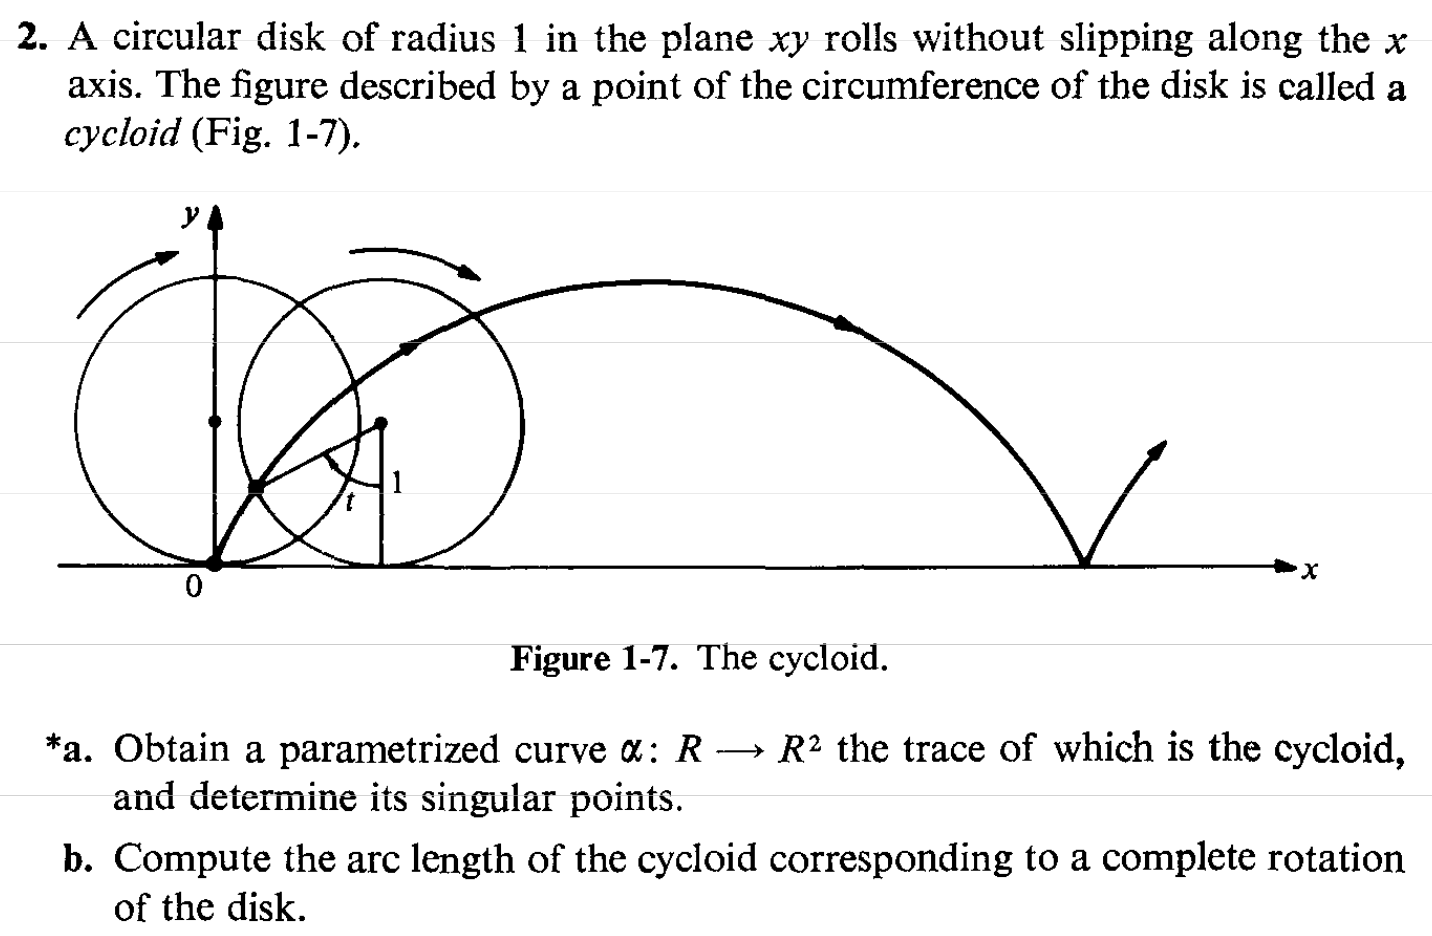
\includegraphics[height=10cm,width=18cm]{1.png}
\end{question}
\begin{proof}
The solution of the question \textbf{a} is 
\begin{align*}
\alpha (t)=(t-\sin t,1-\cos t)
\end{align*}
Compute 
\begin{align*}
\alpha'(t)=(1-\cos t,\sin t)
\end{align*}
and compute
\begin{align*}
\abso{\alpha '(t)}=\sqrt{1-2\cos t +\cos^2 t +\sin^2 t}  = \sqrt{2}\cdot \sqrt{1-\cos t}  
\end{align*}
This implies the singular points are 
\begin{align*}
  \set{2n\pi : n\inz}
\end{align*}


The solution of the question \textbf{b} is then 
\begin{align*}
\int_0^{2\pi} \abso{\alpha '(t)}dt&=\sqrt{2}\int_0^{2\pi} \sqrt{1-\cos t}dt \\
&=\sqrt{2} \int_{0}^{2\pi} \sqrt{2} \abso{\sin \frac{t}{2}}dt  \\
&=2\int_0^{2\pi}\abso{\sin \frac{t}{2}}dt\\
&=4 \int_{0}^{\pi}\sin (\frac{t}{2})dt\\
&=-8 \cos \frac{t}{2}\Big|_0^{\pi}
\end{align*}

\end{proof}
\begin{question}{1-3:4}{}
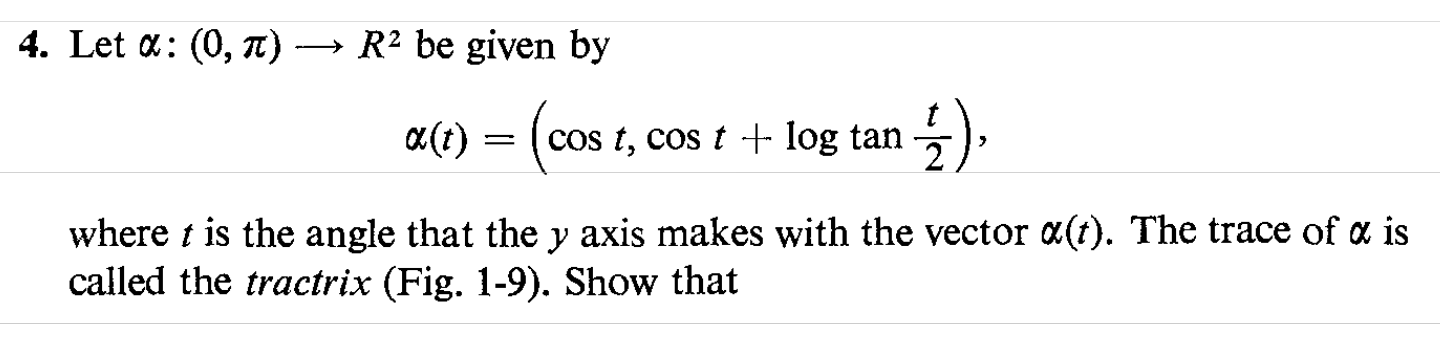
\includegraphics[height=4cm,width=18cm]{3.png}
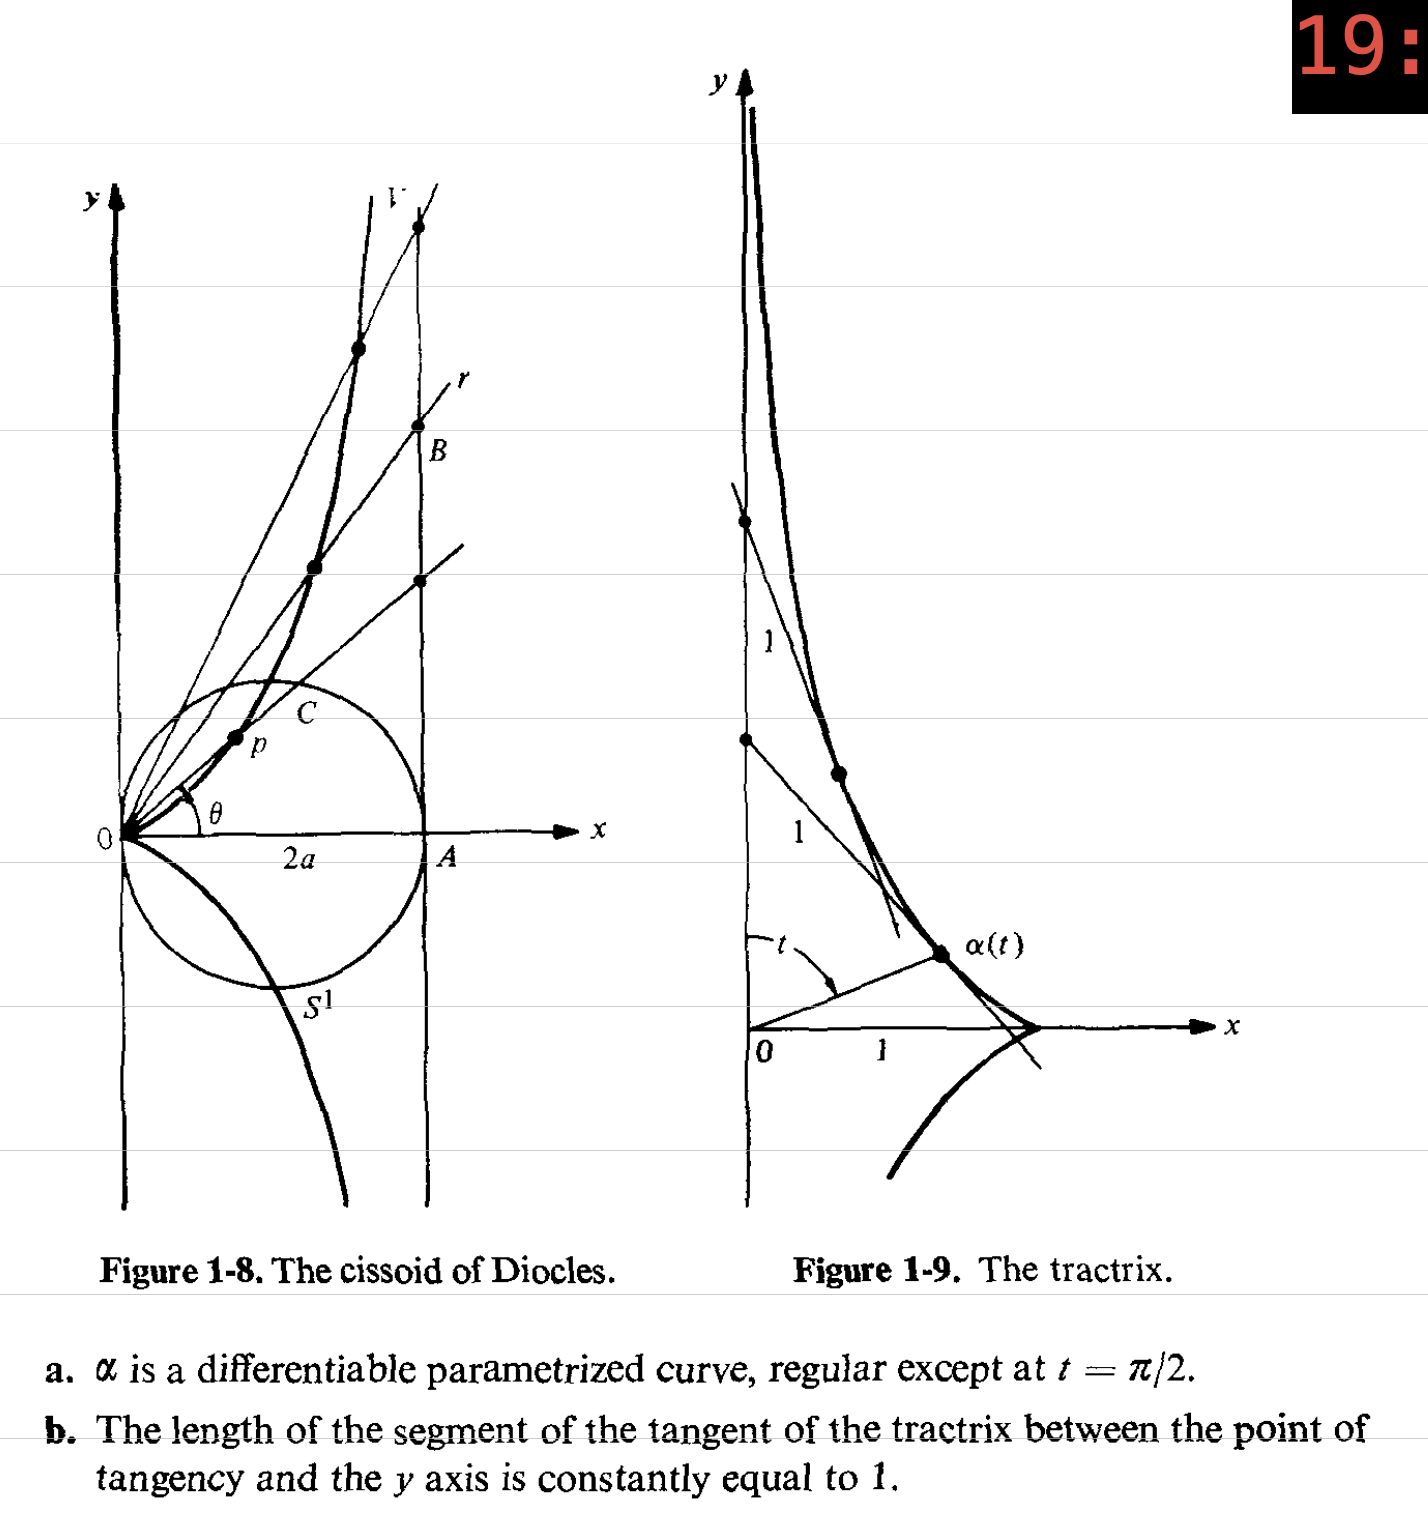
\includegraphics[height=18cm,width=18cm]{2.png}
Typo correction: $\alpha (t)=(\sin t,\cos t + \ln \tan \frac{t}{2})$
\end{question}
\begin{proof}
\textbf{(a)}

Notice that the interval $I$ is  $(0,\pi)$. It is clear that 
\begin{enumerate}[label=(\alph*)]
  \item $\sin t$ is smooth on $\R$
  \item $\cos t$ is smooth on $\R$
  \item $\ln t$ is smooth on $\R$
  $\tan \frac{t}{2}$ is smooth on $I$
\end{enumerate}
Then it follows that $\alpha $ is a differentiable curve.\\

Compute 
\begin{align*}
\alpha '(t)=(\cos t,- \sin t + \frac{1}{\tan \frac{t}{2}} \cdot \sec^2 \frac{t}{2}\cdot \frac{1}{2})
\end{align*}
Because $\cos t=\alpha '_1(t)$ is $0$ on  $I$ only when  $t=\frac{\pi}{2}$, we know $\alpha $ is regular on $I$ except possibly at  $t=\frac{\pi}{2}$.\\

Compute 
\begin{align*}
\alpha '(\frac{\pi}{2})=(0,-1+\frac{1}{1}\cdot 2 \cdot \frac{1}{2} )=(0,0)
\end{align*}
We now conclude $\alpha $ is regular on $I$ except  $\frac{\pi}{2}$. \\

\textbf{(b)}

A useful Identity give us 
\begin{align*}
\alpha '(t)=(\cos t,-\sin t+ \csc t)
\end{align*}
From the following facts
\begin{enumerate}[label=(\alph*)]
  \item the first argument of the segment is from $0$ to  $\sin t =\alpha (t)$
  \item $\alpha_x'(t)=\cos t$
  \item $\frac{\sin t}{\cos t}=\tan t$
\end{enumerate}
We conclude that the length of the segment is 
\begin{align*}
\abso{\tan t}\cdot \abso{\alpha '(t)}&= \abso{\tan t} \cdot \sqrt{\cos ^2 t + \sin^2 t - 2 \sin t \csc t + \csc ^2 t }\\
&=\abso{\tan t} \cdot \sqrt{1-2+\csc ^2 t}\\
&=\abso{\tan t } \cdot \sqrt{\csc ^2 t-1}=\abso{\tan t } \cdot  \sqrt{\cot ^2 t} =1
\end{align*}



\end{proof}
\begin{question}{}{}
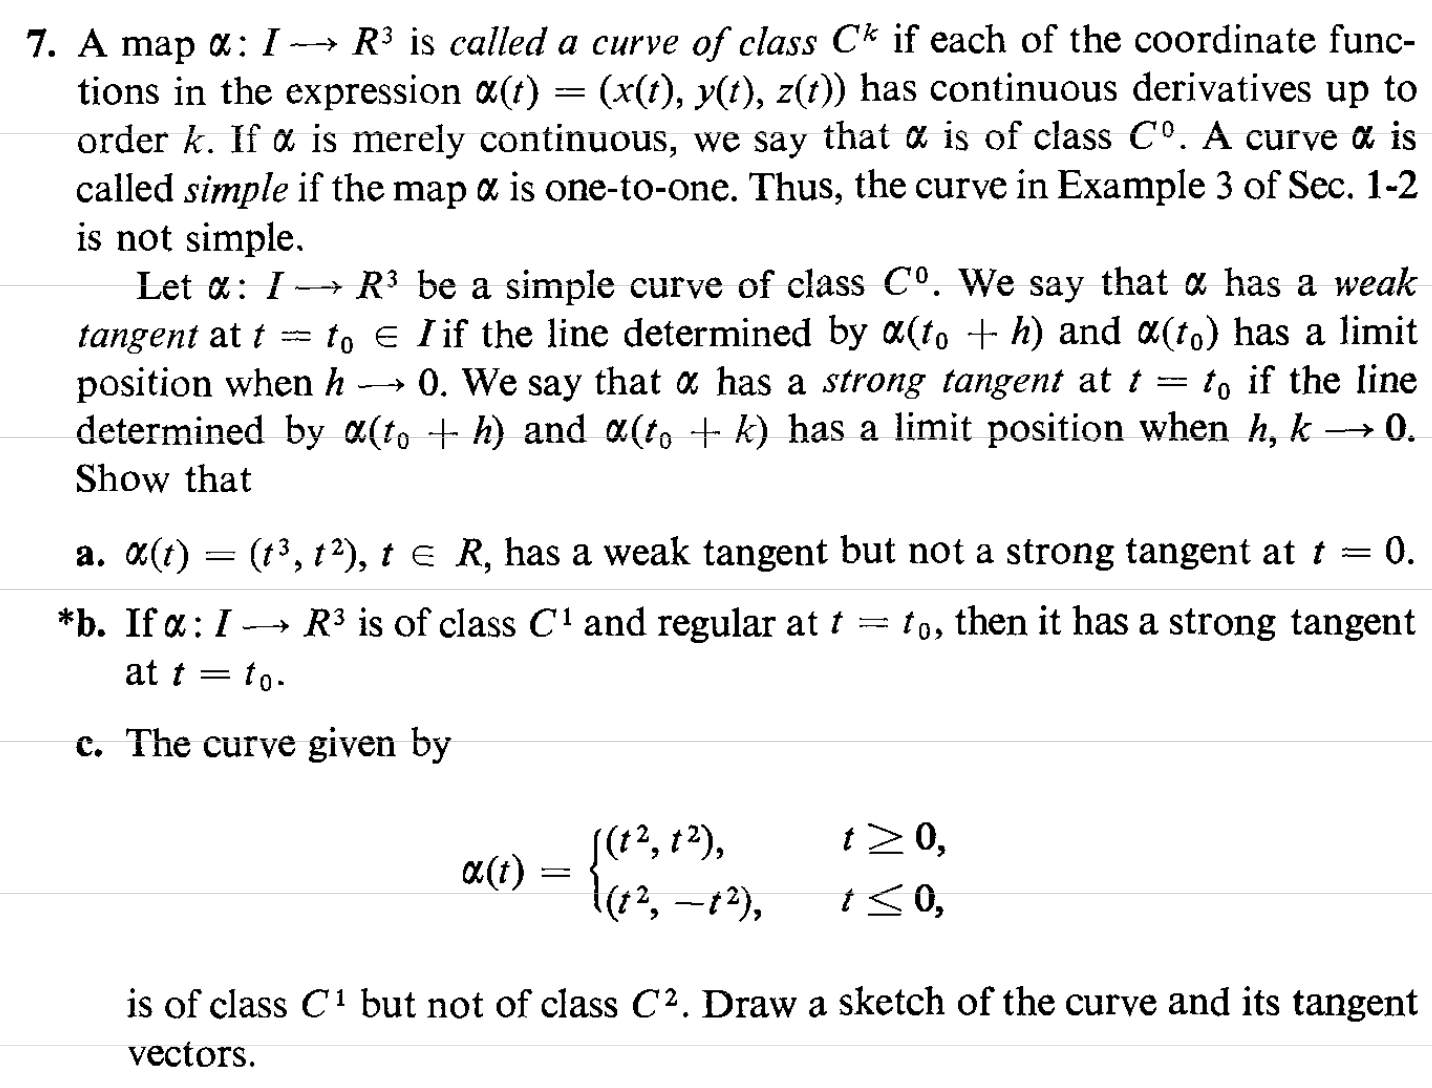
\includegraphics[height=14cm,width=18cm]{qu4}
\end{question}
\begin{proof}
\textbf{(a)}
Let $v=(0,1)$. Compute 
\begin{align*}
\frac{\alpha (t)-\alpha (0)}{\abso{\alpha (t)-\alpha (0)}}\cdot v=\frac{t^2}{\sqrt{t^6+t^4} }=\frac{1}{\sqrt{t^2+1} }\to 1\text{ as }t \to 1
\end{align*}
This implies $\alpha $ has a weak tangent at $t=0$. Now, if $\alpha $ has a strong tangent, we must have 
\begin{align*}
\frac{\alpha (h)-\alpha (-h)}{2h}\cdot v \to 1\text{ or }\to -1
\end{align*}
But this is clearly not the case as 
\begin{align*}
\frac{\alpha (h)-\alpha (-h)}{2h}\cdot v=0\text{ for all $h>0$ }
\end{align*}
So we have the conclusion that $\alpha $ has no strong tangent at $0$.\\


\textbf{(b)} 
By MVT, for each $h,k$ there exists a set of real numbers $\set{c_x,c_y,c_z}$ between $t+h$ and  $t+k$ such that 
 \begin{align*}
\frac{\alpha (t_0+h)-\alpha  (t_0+k)}{h-k}=\Big(x'(c_x),y'(c_y),z'(c_z) \Big)
\end{align*}
Then because 
\begin{align*}
h,k  \to 0 \implies t_0+h ,t_0+k \to t_0 \implies c_x,c_y,c_z \to t_0
\end{align*}
Then from the fact $\alpha $ is of class $C^1$ ($x',y',z'$ are all continuous), we can now deduce 
\begin{align}
\label{ahk}
\frac{\alpha (t_0+h)-\alpha (t_0+k)}{h-k}\to \alpha '(t_0)\text{ as $h,k \to 0$ }
\end{align}
Now, because $\alpha '(t_0)\neq 0$ as $\alpha $ is regular, we see 
\begin{align*}
\lim_{h,k\to 0}\frac{\alpha (t_0+h)-\alpha (t_0+k)}{h-k}\cdot \alpha '(t_0)= \abso{\alpha '(t_0)}^2
\end{align*}
This then implies 
\begin{align*}
\lim_{h,k\to 0}\frac{\alpha (t_0+h)-\alpha (t_0+k)}{\abso{\alpha (t_0+h)-\alpha (t_0+k)}}\cdot \frac{\alpha '(t_0)}{\abso{\alpha '(t_0)}}=1
\end{align*}
which implies the "strong tangent" must always converge to $\alpha '(t_0)$.\\

Notice that the last implication is backed by \myref{Equation}{ahk}\\


\textbf{(c)}\\

From 
\begin{align*}
\alpha (t)=\Big(t^2,\begin{cases}
  t^2& \text{ if $t\geq 0$ }\\
  -t^2& \text{ if $t\leq 0$ }
\end{cases} \Big)
\end{align*}
Compute 
\begin{align*}
\alpha '(t)=\Big(2t,\begin{cases}
  2t& \text{ if $t\geq 0$ }\\
  -2t& \text{ if $t\leq 0$ }
\end{cases} \Big)
\end{align*}
Notice that the derivative at $t=0$ is computed from definition instead of product rule.\\


Now, it is clear that $x',y'$ are continuous. This implies $\alpha  \in C^1$. Yet, we see $y'$ is not differentiable at  $t=0$. This implies  $\alpha \not \in C^2$.\\

The sketch: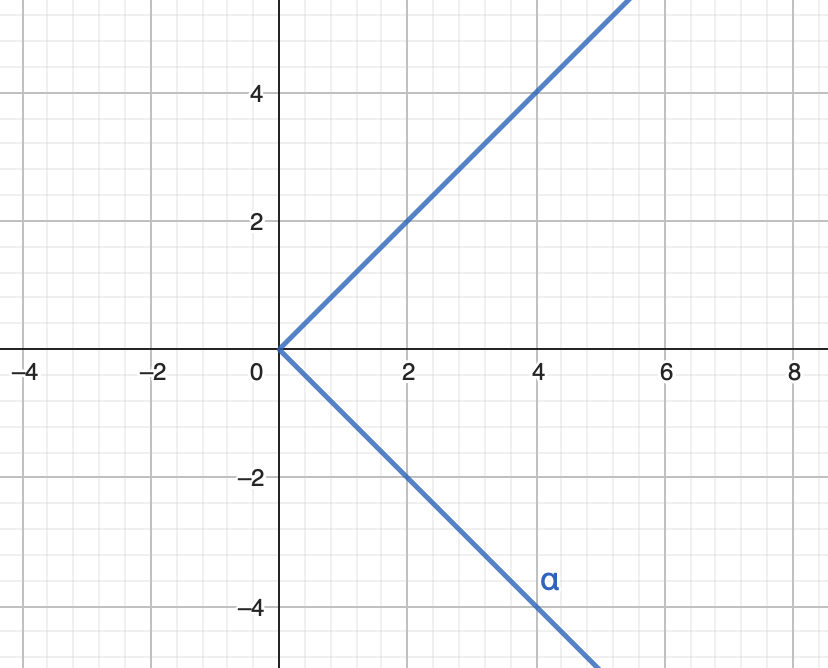
\includegraphics[height=8cm,width=15cm]{qsp}
\end{proof}
\begin{question}{}{}
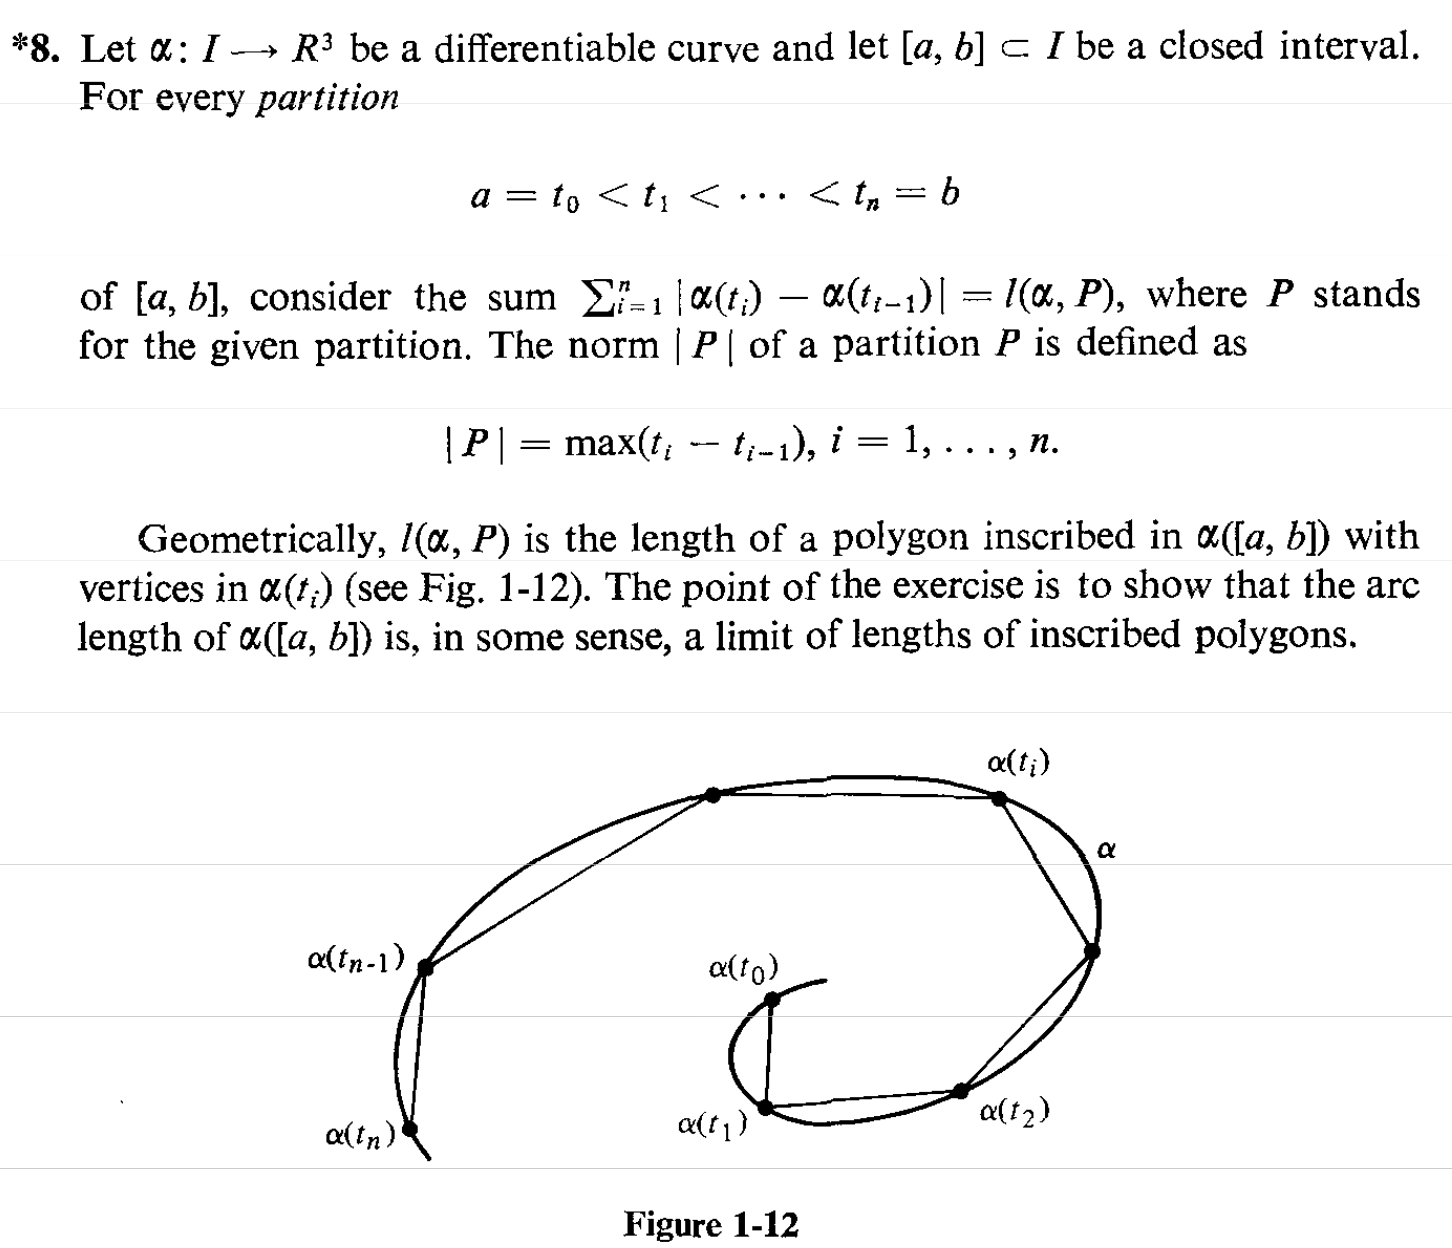
\includegraphics[height=15cm,width=18cm]{qu8}
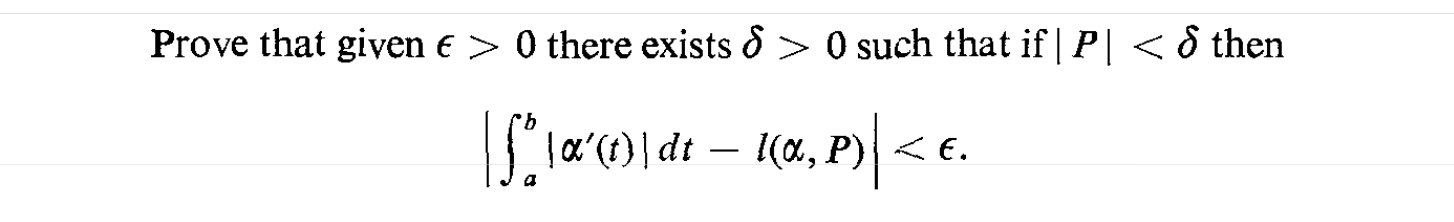
\includegraphics[height=3cm,width=18cm]{qu7}
\end{question}
\begin{proof}
We first prove 
\begin{align*}
\vi{\int_a^b \abso{\alpha '(t)}dt \geq  l(\alpha ,P)}
\end{align*}
By FTC, we have
\begin{align*}
  \abso{\alpha (t_i)-\alpha (t_{i-1})}&=\abso{\int_{t_{i-1}}^{t_i} \alpha '(t)dt}\\
&\leq \int_{t_{i-1}}^{t_i} \abso{\alpha '(t)}dt 
\end{align*}
This then implies 
\begin{align*}
l(\alpha ,P)=\sum \abso{\alpha (t_i)-\alpha (t_{i-1})}\leq \sum \int_{t_{i-1}}^{t_i}\abso{\alpha '(t)}dt=\int_a^b \abso{\alpha '(t)}dt \vdone
\end{align*}
We have reduced the problem into 
\begin{align*}
\blue{\text{ finding $\delta$ such that }\forall P: \abso{P}<\delta , \int_a^b \abso{\alpha '(t)}dt - l(\alpha ,P)<\epsilon }
\end{align*}


Because $\alpha '$ is uniformly continuous on $[a,b]$ ($\because$ continuous function on compact domain is uniformly continuous), we know there exists $\delta ' $ such that 
\begin{align*}
\abso{\alpha '(s)-\alpha '(t)}< \frac{\epsilon }{2(b-a)}\text{ if $\abso{s-t}<\delta'$ }
\end{align*}
We claim 
\begin{align*}
\blue{\text{ such $\delta'$ works }}
\end{align*}
Let $\abso{P}<\delta$, and let $s_i \in [t_{i-1},t_i]$. Because $\abso{s_i-t_i}<\delta$, we have
\begin{align}
\label{siti}
\abso{\alpha '(s_i)-\alpha '(t_i)}<\frac{\epsilon}{2(b-a)}
\end{align}
This give us 
\begin{align*}
\abso{\alpha '(s_i)}<\abso{\alpha '(t_i)} + \frac{\epsilon}{2(b-a)}
\end{align*}
Now, we can deduce 
\begin{align*}
  \int_{t_{i-1}}^{t_i} \abso{\alpha '(s)}ds&\leq   \abso{\alpha '(t_i)}\Delta t_i+ \frac{\epsilon }{2(b-a)}\Delta t_i\\
  &=\int_{t_{i-1}}^{t_i}\abso{\alpha '(t_i)}dt + \frac{\epsilon}{2(b-a)}\Delta t_i\\
 &=\abso{\int_{t_{i-1}}^{t_i} \alpha '(t_i)dt}+ \frac{\epsilon }{2(b-a)}\Delta t_i\\
  &=\abso{\int_{t_{i-1}}^{t_i} \alpha' (t_i)-\alpha '(t)dt + \int_{t_{i-1}}^{t_i} \alpha '(t)dt }+ \frac{\epsilon}{2(b-a)}\Delta t_i \\
  &\leq  \abso{\int_{t_{i-1}}^{t_i} \alpha '(t_i)-\alpha' (t)dt}+ \abso{\int_{t_{i-1}}^{t_i} \alpha '(t)dt}+\frac{\epsilon}{2(b-a)}\Delta t_i \\
  &\leq \frac{\epsilon}{2(b-a)}\Delta t_i + \abso{\alpha (t_i)-\alpha (t_{i-1})}+\frac{\epsilon}{2(b-a)}\Delta t_i\\
  &=\abso{\alpha (t_i)-\alpha (t_{i-1})}+ \frac{\epsilon }{b-a}\Delta t_i
\end{align*}
Notice that the last inequality follows from \myref{Equation}{siti}. The long deduction above then give us 
\begin{align*}
  \int_{a}^b \abso{\alpha '(t)}dt&\leq \sum \abso{\alpha (t_i)-\alpha (t_{i-1})}+ \frac{\epsilon}{b-a} (b-a)\\
&=l(\alpha ,P)+\epsilon 
\end{align*}
Then we have 
\begin{align*}
\int_a^b \abso{\alpha '(t)}dt -l(\alpha ,P)\leq \epsilon \bdone
\end{align*}
\end{proof}
\begin{question}{}{}
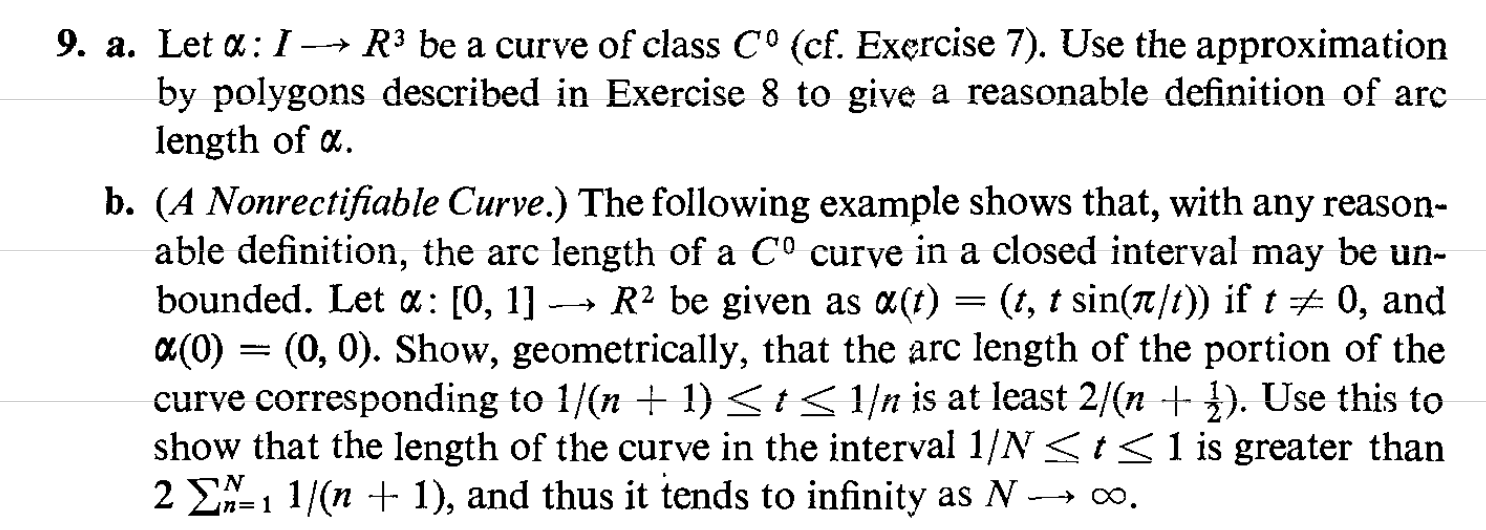
\includegraphics[height=7cm,width=18cm]{qu6}
\end{question}
\begin{proof}
\textbf{(a)} 
Suppose $I=[a,b]$. Define arc length by 
\begin{align*}
\sup_{P} l(P,\alpha )\text{ where $\sup $ runs over all partition $P$ of $[a,b]$  }
\end{align*}

\textbf{(b)}\\

Geometrically, we know the arc length of the portion of the curve corresponding to $t \in [\frac{1}{n+1},\frac{1}{n}]$ must be greater than 
\begin{align}
\label{19b}
\abso{\alpha \big(\frac{1}{n}\big)-\alpha \big(\frac{1}{n+\frac{1}{2}}\big)}+\abso{\alpha \big(\frac{1}{n+1} \big)-\alpha \big(\frac{1}{n+\frac{1}{2}} \big)}
\end{align}
WOLG of $n$ being odd or even, Compute 
\begin{align*}
\abso{\alpha \big(\frac{1}{n} \big)-\alpha \big(\frac{1}{n+\frac{1}{2}} \big)}&=\abso{(\frac{1}{n},0)-(\frac{1}{n+\frac{1}{2}},\frac{1}{n+\frac{1}{2}})}\\
&=\sqrt{\big(\frac{1}{n}-\frac{1}{n+\frac{1}{2}} \big)^2 +\big(\frac{1}{n+\frac{1}{2}} \big)^2} \\
&=\sqrt{\frac{1}{n^2}-\frac{4}{n(2n+1)}+\frac{8}{(2n+1)^2}} \\
&=\sqrt{\frac{(2n+1)^2-4n(2n+1)+8n^2}{n^2(2n+1)^2}} \\
&=\sqrt{\frac{4n^2+1}{n^2(2n+1)^2}}\\
&=\frac{\sqrt{4n^2+1} }{n(2n+1)}\geq \frac{\sqrt{4n^2} }{n(2n+1)}=\frac{2}{2n+1}
\end{align*}
and compute 
\begin{align*}
\abso{\alpha \big(\frac{1}{n+\frac{1}{2}} \big)-\alpha \big(\frac{1}{n} \big)}&=\abso{(\frac{1}{n+\frac{1}{2}},\frac{1}{n+\frac{1}{2}})-(\frac{1}{n+1},0)}\\
&=\sqrt{\big(\frac{1}{n+1}-\frac{1}{n+\frac{1}{2}} \big)^2 + \big(\frac{1}{n+\frac{1}{2}} \big)^2} \\
&=\sqrt{\frac{1}{(n+1)^2}-\frac{4}{(n+1)(2n+1)}+\frac{8}{(2n+1)^2}}\\
&=\sqrt{\frac{(2n+1)^2 -4(n+1)(2n+1)+8(n+1)^2}{(n+1)^2(2n+1)^2}}\\
&=\sqrt{\frac{4n^2+8n+5}{(n+1)^2(2n+1)^2}}\\
&\geq \frac{\sqrt{4n^2+8n+4} }{(n+1)(2n+1)}=\frac{2}{2n+1}
\end{align*}
From the computation and \myref{Equation}{19b}, it is now clear that the arc length of the portion of the curve corresponding to $ t \in [\frac{1}{n+1},\frac{1}{n}]$ is at least $\frac{2}{n+\frac{1}{2}}$. With simple addition, this then implies the arc length of the curve in the interval $[\frac{1}{N},1]$ is at least 
\begin{align*}
  \sum_{n=1}^{N-1} \frac{2}{2n+1}=2 \sum_{n=1}^{N-1}\frac{1}{2n+1}
\end{align*}
The number is clearly greater than 
\begin{align*}
2 \sum_{n=1}^{N-1}\frac{1}{2n+2}
\end{align*}
which equals to 
\begin{align*}
\sum_{n=1}^{N-1}\frac{1}{n+1}
\end{align*}
The series diverge to $+\infty$ as $N$ to  $\infty$. 
\end{proof}
\begin{theorem}
\label{IDP}
\textbf{(Integrating the Dot Product)} Given a curve $u:[a,b]\rightarrow \R^n$ and a vector $v \in\R^n$, suppose 
\begin{enumerate}[label=(\alph*)]
  \item $u$ is differentiable on $(a,b)$ 
  \item $u$ is continuous on  $[a,b]$
\end{enumerate}
We have 
\begin{align*}
\int_a^b u'(t)\cdot v dt=
\Big(\int_a^b u'(t)dt \Big)\cdot v= \big(u(b)-u(a) \big)\cdot v
\end{align*}
\end{theorem}
\begin{proof}
\begin{align*}
\int_a^b u'(t)\cdot vdt&=\int_a^b \sum_{k=1}^n u'_k(t)\cdot v_k dt \\
&=\sum_{k=1}^n  \int_a^b u'_k(t)\cdot v_k dt\\
&=\sum_{k=1}^n v_k \int_a^b u'_k(t)dt\\
&=v\cdot \Big(\int_a^b u'(t)dt \Big)
\end{align*}
\end{proof}
\begin{question}{}{}
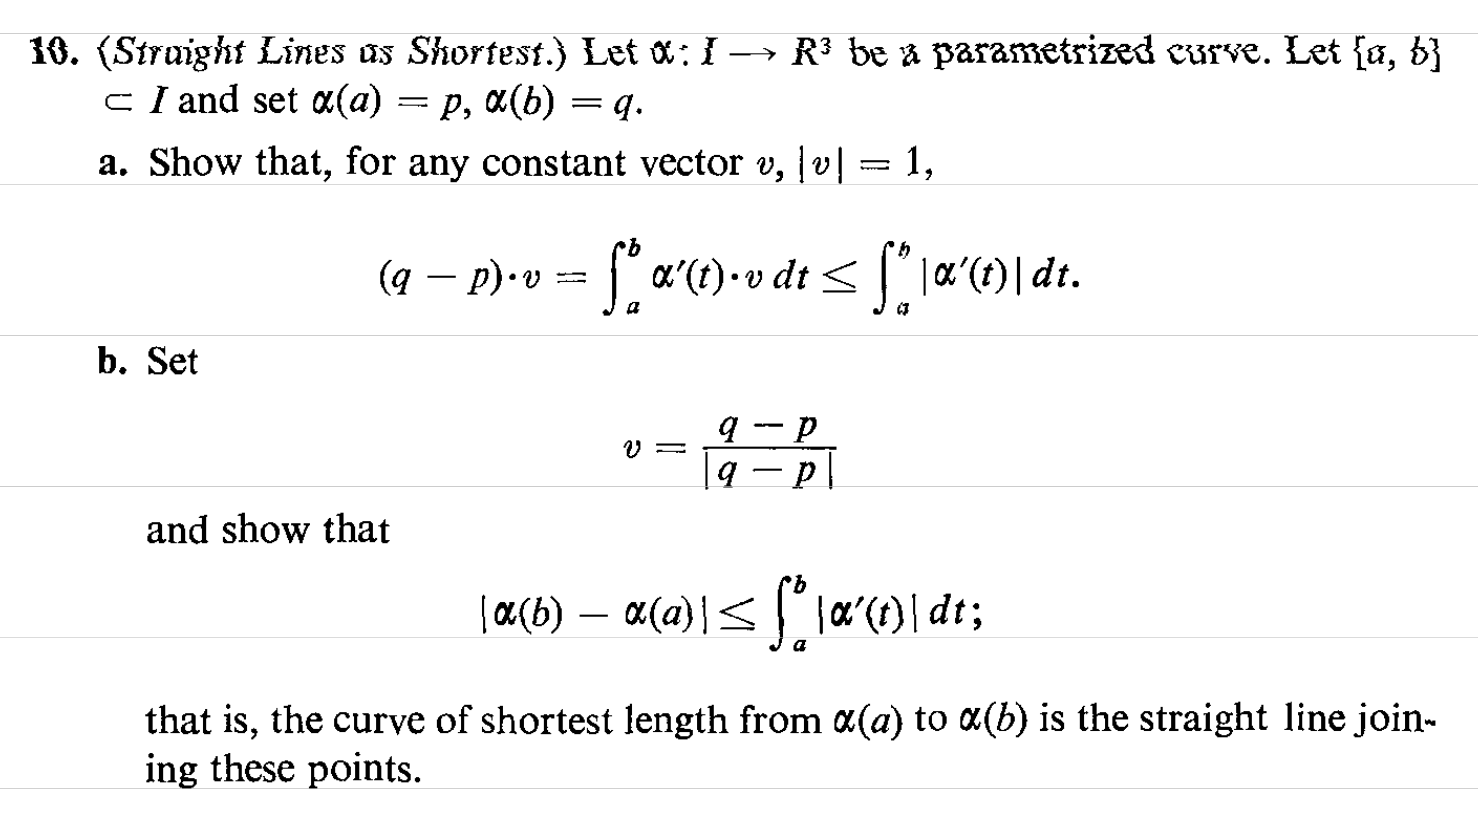
\includegraphics[height=10cm,width=18cm]{qu5}
\end{question}
\begin{proof}
\textbf{(a)}\\


The first equality 
\begin{align*}
  (q-p)\cdot v=\int_a^b \alpha '(t)\cdot vdt
\end{align*}
follows directly from \myref{Theorem}{IDP}.\\

Now, by Cauchy-Schwarz inequality, we have 
\begin{align*}
  \abso{\alpha '(t)\cdot v} \leq \abso{\alpha '(t)}\cdot \abso{v}
\end{align*}
This then give us 
\begin{align*}
\alpha '(t)\cdot v\leq \abso{\alpha '(t)\cdot v}\leq \abso{\alpha '(t)}\cdot \abso{v}=\abso{\alpha '(t)}
\end{align*}
We now have 
\begin{align*}
\int_a^b \alpha '(t)\cdot v \leq \abso{\alpha '(t)}dt
\end{align*}
as desired.\\

\textbf{(b)}

The first inequality tell us that if $v$ is a constant and $\abso{v}=1$, we have 
\begin{align*}
  (q-p)\cdot v \leq \int_a^b \abso{\alpha '(t)}dt
\end{align*}
If $v=\frac{q-p}{\abso{q-p}}$, it is clear that $v$ is a constant and  $\abso{v}=1$, and at the same time, we have 
\begin{align*}
  (q-p)\cdot v=\frac{(q-p)\cdot (q-p)}{\abso{q-p}}=\frac{\abso{q-p}^2}{\abso{q-p}}=\abso{q-p}
\end{align*}
We now have 
\begin{align*}
\abso{q-p}=(q-p)\cdot v \leq \int_a^b \abso{\alpha '(t)}dt
\end{align*}
from the first inequality 
\end{proof}
\begin{question}{}{}
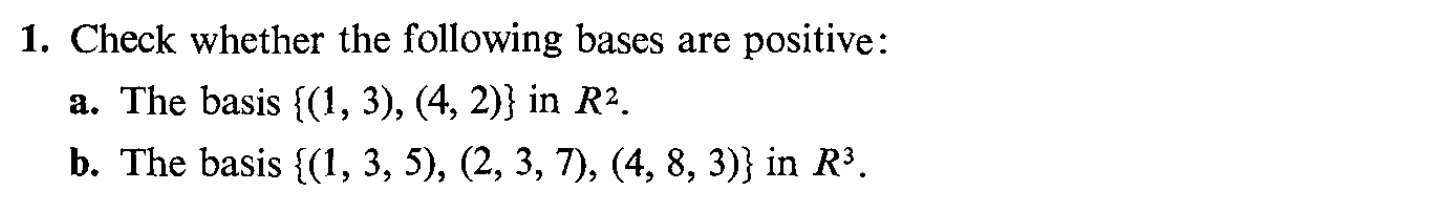
\includegraphics[height=2cm,width=18cm]{qu9}
\end{question}
\begin{proof}
Compute 
\begin{align*}
\begin{vmatrix} 
  1 & 4 \\
  3 & 2
\end{vmatrix}=-10
\end{align*}
and compute 
\begin{align*}
\begin{vmatrix}
  1& 2 & 4 \\
  3 & 3 & 8 \\
  5 & 7 & 3
\end{vmatrix}=-9
\end{align*}
Both bases are negatively oriented. 
\end{proof}
\begin{question}{}{}
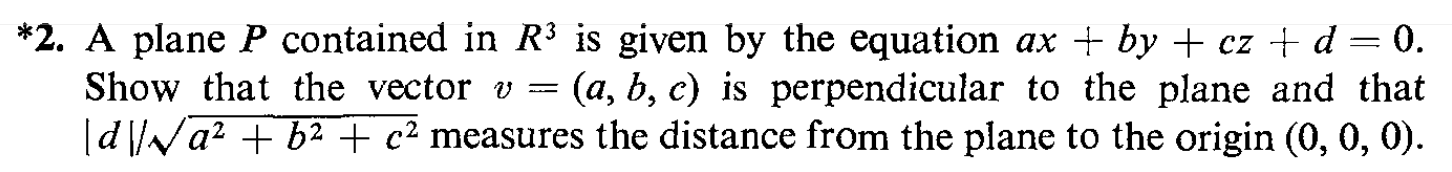
\includegraphics[height=2cm,width=18cm]{qu10}
\end{question}
\begin{proof}
Arbitrarily pick two points $u,w$ in  $P$. We wish to show 
\begin{align*}
  \vi{v\cdot (u-w)=0}
\end{align*}
Because $v=(a,b,c)$ and 
\begin{align*}
\begin{cases}
  au_1+b u_2+cu_3=-d
  aw_1+b w_2+cw_3=-d
\end{cases}
\end{align*}
We see
\begin{align*}
v\cdot (u-w)&= a(u_1-w_2)+b(u_2-w_2)+c(u_3-w_2)\\
&=(-d)-(-d)=0\vdone
\end{align*}
To measure the distance between $P$ and the origin, we wish to find a vector $u$ such that  $u\perp P$ and $u \in P$. We know that $u$ must be linearly dependent with  $v=(a,b,c)$, since the dimension of  $P^\perp$ is $1$. Then, we can write
\begin{align*}
u=c_0(a,b,c)\text{ for some $c_0\inr$ }
\end{align*}
Because $u \in P$, we know 
\begin{align*}
c_0a^2+c_0b^2+c_0c^2+d=0
\end{align*}
This tell us 
\begin{align*}
c_0=\frac{-d}{a^2+b^2+c^2}
\end{align*}
We now see that the distance $\abso{u}$ between $P$ and origin is 
\begin{align*}
\abso{u}=\abso{c_0}\cdot \sqrt{a^2+b^2+c^2}= \frac{\abso{d}}{\sqrt{a^2+b^2+c^2} }
\end{align*}

\end{proof}
\begin{question}{}{}
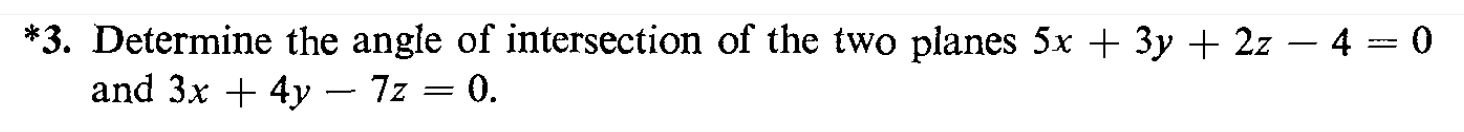
\includegraphics[height=2cm,width=18cm]{qu11}
\end{question}
\begin{proof}
From last question, we know the two vectors $u,v$ that are respectively perpendicular to  $P:5x+3y+2z-4=0$ and  $Q:3x+4y-7z=0$ respectively have the direction 
 \begin{align*}
   (5,3,2)\text{ and }(3,4,-7)
\end{align*}
Then, we see the angle of the intersection are 
\begin{align*}
\arccos \frac{5\cdot 3+3\cdot 4 +2 \cdot (-7)}{\sqrt{5^2+3^2+2^2} \sqrt{3^2+4^2+7^2} }=\arccos \frac{13}{\sqrt{38}\sqrt{71}  }
\end{align*}
Notice that this angle is smaller than $\frac{\pi}{2}$ as we intend it to be. 
\end{proof}
\begin{question}{}{}
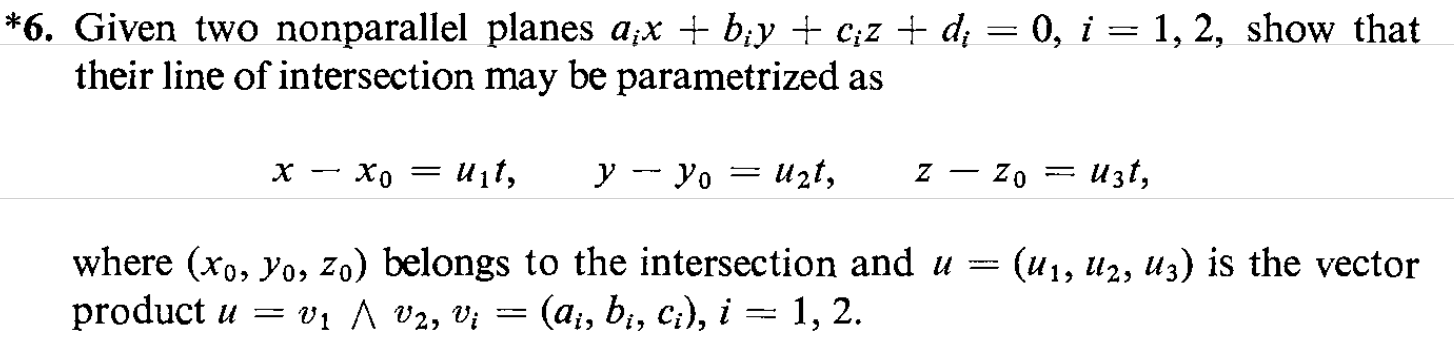
\includegraphics[height=4cm,width=18cm]{qu12}
\end{question}
\begin{proof}
Let $v=(x,y,z)$ be a point on the line of intersection.  We see the vector  $v-(x_0,y_0,z_0)$ lies on both planes, and thus must be perpendicular to $(a_1,b_1,c_1)=v_1$ and $(a_2,b_2,c_2)=v_2$ thus satisfying 
\begin{align*}
v-(x_0,y_0,z_0)=tv_1\times v_2=tu\text{ for some $t\inr$ }
\end{align*}
sine in $\R^3$, the only direction perpendicular to both  $v_1,v_2$ is  $v_1\times v_2$. We can rewrite the above equation of course into 
\begin{align*}
x-x_0=u_1t,y-y_0=u_2t,z-z_0=u_3t
\end{align*}
\end{proof}
\section{HW2}

\begin{question}{}{}
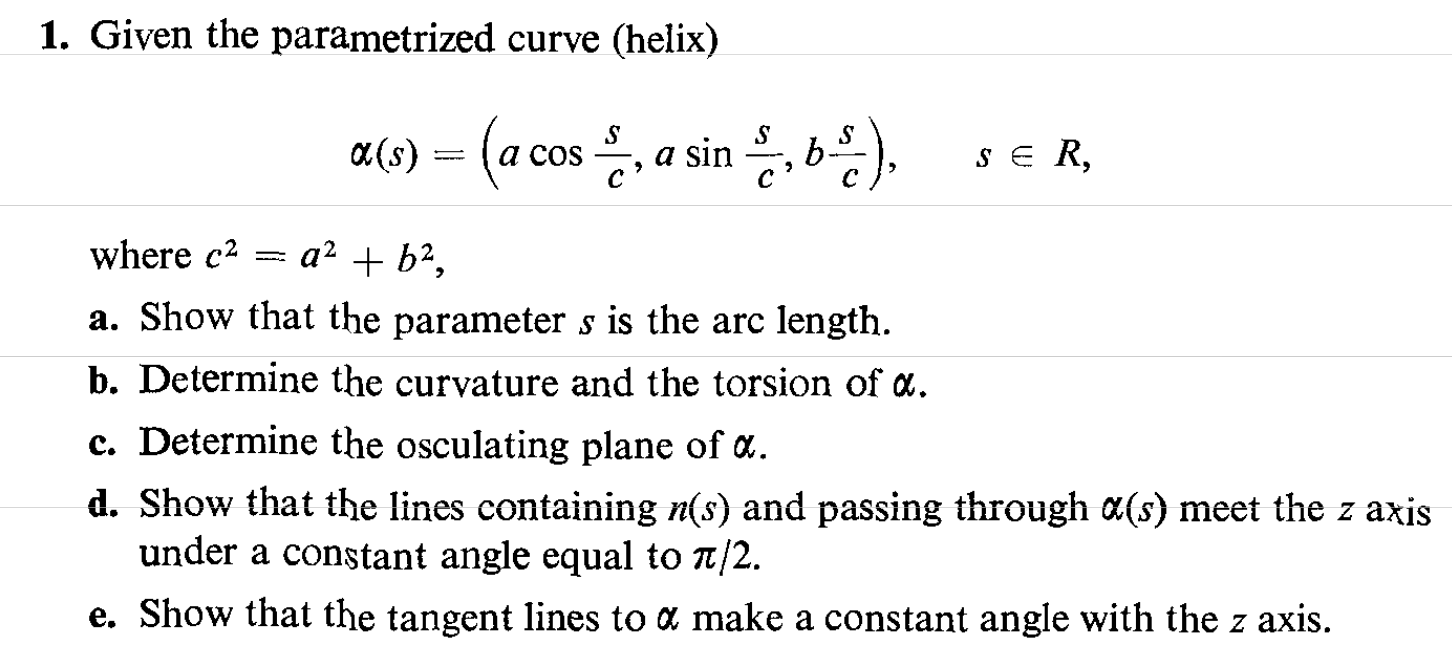
\includegraphics[height=10cm,width=18cm]{hw2q5}
\end{question}
\begin{proof}
\textbf{(a)}
By computation 
\begin{align*}
\alpha '(s)=(\frac{-a}{c} \sin \frac{s}{c},\frac{a}{c}\cos \frac{s}{c},\frac{b}{c}) 
\end{align*}
So 
\begin{align*}
\abso{\alpha '(s)}=\sqrt{\frac{a^2+b^2}{c^2}}=1\hspace{3cm}(\because \text{ $\sin^2+\cos^2=1$ })
\end{align*}
This shows $\alpha $ is parametrized by arc-length.\\

\textbf{(b)}
By computation 
\begin{align*}
\alpha ''(s)=\Big(\frac{-a}{c^2} \cos \frac{s}{c}, \frac{-a}{c^2} \sin \frac{s}{c},0\Big)
\end{align*}
Then because $\alpha $ is parametrized by arc-length, we have 
\begin{align*}
\kappa(s)=\abso{\alpha ''(s)}&= \sqrt{\frac{a^2}{c^4}}\\
&=\frac{\abso{a}}{c^2}
\end{align*}
By computation 
\begin{align*}
\alpha '''(s)=\Big(\frac{a}{c^3}\sin \frac{s}{c}, \frac{-a}{c^3} \cos \frac{s}{c},0 \Big)
\end{align*}
Then using the identity of torsion, we have 
\begin{align*}
\tau (s)&=- \frac{- \big(\alpha '(s)\times \alpha ''(s) \big)\cdot \alpha '''(s)}{\abso{\kappa (s)}^2}\\
&=-\frac{\frac{a^2b}{c^6}}{\frac{a^2}{c^4}}\\
&=\frac{b}{-c^2}
\end{align*}
\textbf{(c)}
Fix $s$. Define a set $A$  by 
\begin{align*}
A=\text{span}\Big(\alpha '(s),\alpha ''(s) \Big)
\end{align*}
The osculating plane of $\alpha $ at $s$ is then exactly 
\begin{align*}
\set{a+\alpha (s): a \in A}
\end{align*}
\textbf{(d)}
Because $\alpha ''(s)$ by our computation is valued $0$ in  $z$-opponent, we know if the line containing  $N$ and passing through $\alpha $ meet the $z$ axis, it must be under a constant angle equal to  $\frac{\pi}{2}$. (use dot product to check this fact.).\\

Now, we only have to prove that the line does meet the $z$-axis. See that 
\begin{align*}
\alpha + c^2 \alpha ''=\Big(0,0,b\frac{s}{c} \Big)
\end{align*}
and we are done.

\textbf{(e)}
Observe that 
\begin{align*}
\alpha ' \cdot \Big(0,0,1 \Big)=\frac{b}{c}\text{ is a constant }
\end{align*}
This together with the fact $\abso{\alpha '}$ is a constant show that the angle between the tangent to $\alpha $ and $z$-axis is a constant.

\end{proof}
\begin{question}{}{}
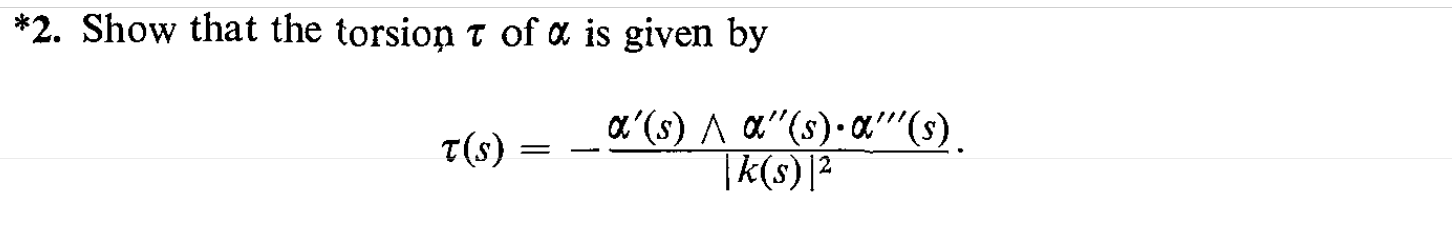
\includegraphics[height=3cm,width=18cm]{hw2q4}
\end{question}
\begin{theorem}
\textbf{(Identity of Torsion)} Given a parametrized by arc-length cruve $\alpha  :I \rightarrow \R^3$, we have 
\begin{align*}
\tau(s)=-\frac{\big(\alpha '(s)\times \alpha ''(s) \big)\cdot \alpha '''(s)}{\kappa ^2 (s)}
\end{align*}
\end{theorem}
\begin{proof}
Because $\underline{\alpha  \text{ is parametrized by arc-length}}$, we have 
\begin{align*}
  \alpha '(s)=T(s)
\end{align*}
We first show 
\begin{align}
\label{A'''}
\vi{\alpha ''(s)=\kappa (s)N(s)}
\end{align}
Compute 
\begin{align*}
N(s)&=\frac{T'(s)}{\abso{T'(s)}}\\
&=\frac{\alpha ''(s)}{\abso{\alpha ''(s)}}=\frac{\alpha ''(s)}{\kappa (s)}\vdone
\end{align*}
We now show 
\begin{align*}
\blue{\alpha '''(s)=\kappa(s)\big(-(\tau B)(s)-(\kappa T)(s)\big)+\kappa'(s)N(s) }
\end{align*}
By \myref{Equation}{A'''} and Frenet Formula, we have 
\begin{align*}
\alpha '''(s)&=\kappa'(s)N(s)+\kappa(s)N'(s)\\
&=\kappa'(s)N(s)+\kappa(s)\big(- (\tau B)(s)-(\kappa T)(s) \big)\bdone
\end{align*}
Lastly, we verify 
\begin{align*}
-\frac{\big(\alpha '(s)\times \alpha ''(s) \big)\cdot \alpha '''(s)}{\kappa^2(s)}&=-\frac{(T\times \kappa N)\cdot \Big( \kappa \big(-\tau B-\kappa T \big)+\kappa ' N\Big) }{\kappa ^2}\\
&=-\frac{-\kappa^2 \tau (T\times N)\cdot B }{\kappa^2}\hspace{1cm}(\because T\times N \cdot (T\text{ or }N)=0)\\
&=\tau 
\end{align*}
\end{proof}
\begin{question}{}{}
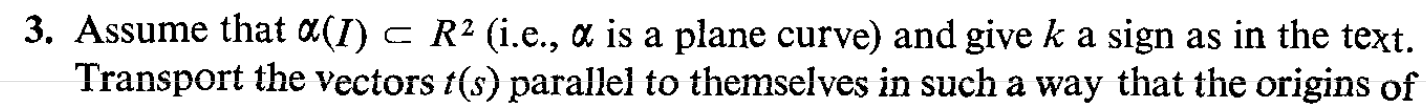
\includegraphics[height=1.5cm,width=18cm]{hw2q3}
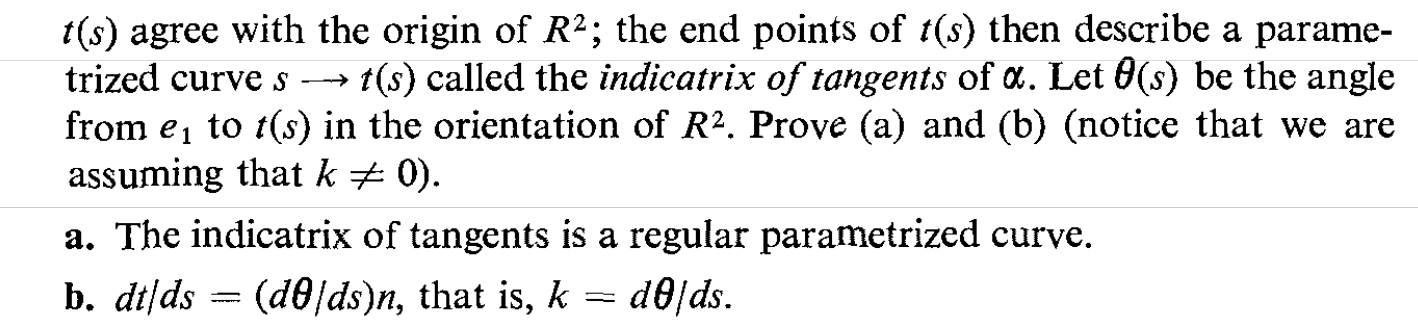
\includegraphics[height=4cm,width=18cm]{hw2q2}
\end{question}
\begin{proof}
\textbf{(a)}\\

The indicatrix of tangents $\gamma :I \rightarrow \R^2$ is defined by 
\begin{align*}
\gamma = \frac{\alpha '(s)}{\abso{\alpha '(s)}}
\end{align*}
Express $\alpha '(s)$ by 
\begin{align*}
\alpha ' \triangleq (x,y)
\end{align*}
To show $\gamma $ is regular. We wish to show 
\begin{align*}
  \vi{\gamma '(s)\neq 0\text{ for all $s \in I$ }}
\end{align*}
Express $\gamma $ by 
\begin{align*}
\gamma =\frac{(x,y)}{\sqrt{x^2+y^2} }
\end{align*}
Then, we see the $x$-component of  $\gamma '(s)$ is 
\begin{align*}
\gamma '(s)\Big|_x= \frac{x'y^2}{(x^2+y^2)^{\frac{3}{2}}}
\end{align*}
With similar computation on the $y$-component, we now arrive at 
 \begin{align*}
\gamma '(s)=\frac{\Big(x'y^2,y'x^2 \Big)}{(x^2+y^2)^{\frac{3}{2}}}
\end{align*}
Now, for a contradiction, \As{$\gamma '(s)=0$ for some $s$}. Then one of the three things below must happen 
\begin{enumerate}[label=(\alph*)]
  \item $x'=y'=0$ 
  \item $y^2=x^2=0$ 
  \item $x'=x^2=0$ WLOG
\end{enumerate}
Because $(x,y)=\alpha '$ and $\alpha $ is parametrized by arc-length and  curvature is non-zero by premise, we know it can not happen $\alpha ''=(x',y')=0$.\\

Because $(x,y)=\alpha '$ and $\alpha $ is parametrized by arc-length, we also know it can not happen $\alpha '=(x,y)=0$.\\

Now, we are given the hypothesis $x'=x^2=0$. Because $\alpha$ is parametrized by arc-length, from $x=0$, we know  $y=\pm 1$.  Then because $\abso{\alpha '}$ is constant, we can deduce
\begin{align*}
  0&=(x',y')\cdot (x,y)\\
  &=(0,y')\cdot (0,\pm 1)
\end{align*}
This show us $y'=0$, which is impossible, since if  $(x',y')=0$ then the curvature is $0\tCaC\vdone$\\

\textbf{(b)}
The functions $\theta : [0,l]\rightarrow \R$, is defined by  
\begin{align*}
 T= (x,y)\triangleq (\cos \theta, \sin \theta)
\end{align*}
By Frenet Formula, we have 
\begin{align}
\label{kN=}
\kappa N=T'= \theta' (- \sin \theta , \cos \theta)
\end{align}
Because $\abso{(-\sin \theta, \cos \theta)}=1$ and $(- \sin \theta ,\cos \theta)\cdot T=0$ and  
 \begin{align*}
\begin{vmatrix} 
  \cos \theta & \sin \theta\\
  - \sin \theta & \cos \theta
\end{vmatrix}=1
\end{align*}
we can identify $(-\sin \theta, \cos \theta)=N$. Then from \myref{Equation}{kN=}, we now can deduce 
\begin{align*}
\kappa =\theta' 
\end{align*}



\end{proof}
\begin{question}{}{}
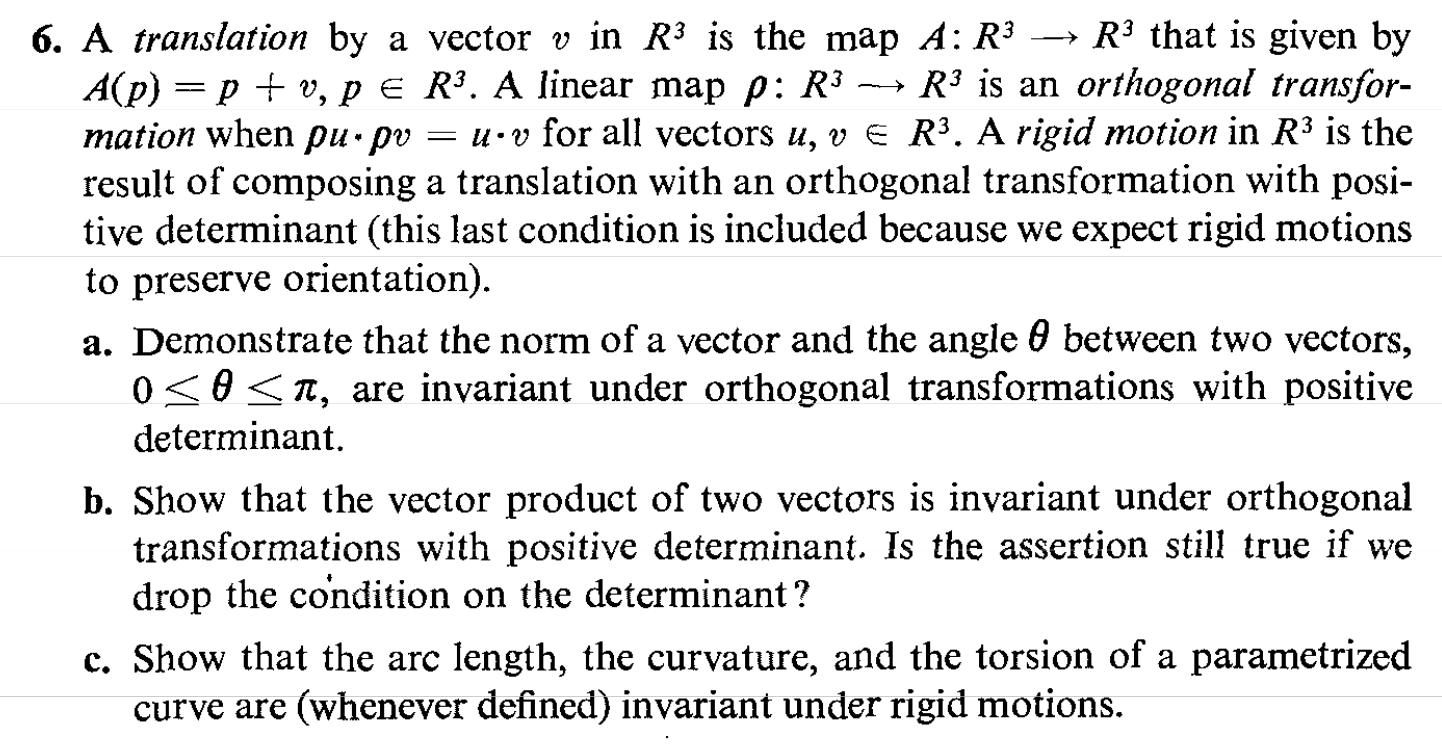
\includegraphics[height=10cm,width=18cm]{hw2q1}
\end{question}
\begin{proof}
Let $A$ be a translation and $\rho$ be an orthogonal transformation.\\

\textbf{(a)}
Observe
\begin{align*}
\norm{v}&= \sqrt{ v \cdot  v} \\
&=\sqrt{\rho v \cdot \rho v}\\
&=\norm{\rho v}
\end{align*}
Because $\theta$ is given by 
\begin{align*}
\theta= \arccos \frac{v \cdot w}{ \abso{v}\cdot \abso{w}}
\end{align*}
and because norm is invariant under orthogonal transformation, from the definition of orthogonal transformation, we now see 
 \begin{align*}
\theta &= \arccos \frac{v \cdot w}{\abso{v}\cdot \abso{w}}\\
&=\arccos \frac{\rho v \cdot \rho w}{\abso{v}\cdot \abso{w}}\\
&=\arccos \frac{\rho v \cdot \rho w}{\abso{\rho v}\cdot \abso{\rho w}}=\theta_\rho\\
\end{align*}
where $\theta_\rho$ is the angle between $\rho v$ and $\rho w$. \\

\textbf{(b)}
Fix $v,w \inr^3$ and a positive determinant orthogonal transformation $\rho$. We wish to show 
\begin{align*}
\vi{\rho v \times \rho w = \rho(v \times w)}
\end{align*}
We can reduce the problem into proving 
\begin{align*}
\vi{\rho v \times \rho w \cdot z = \rho (v \times w) \cdot z\text{ for all $z \inr^3$ }}
\end{align*}
Fix $z \inr^3$. Because $\rho$ has non-zero determinant, we know there exists $z' \inr^3$ such that 
\begin{align*}
\rho z'=z
\end{align*}
Now, because orthogonal transformation has determinant  $\pm 1$ and we have know  $\rho$ has positive determinant, we know
\begin{align*}
\rho v \times \rho w \cdot z&=\rho v \times \rho w \cdot \rho z'\\
&=\begin{vmatrix} 
\rho v\\
\rho w\\
\rho z'\end{vmatrix} \\
&= \begin{vmatrix} 
  \rho v & \rho w & \rho z'
\end{vmatrix}\hspace{1cm}(\because \text{det}A=\text{det}A^t)\\
&=\abso{\rho} \cdot \begin{vmatrix} 
  v & w & z'
\end{vmatrix}\hspace{1cm}(\because \text{det}A\text{det}B=\text{det}AB)\\
&=\begin{vmatrix} 
v \\
w \\
z'
\end{vmatrix}\hspace{1cm}(\because \text{det}\rho=1)\\
&=v \times w \cdot z'\\
&=\rho (v \times w) \cdot \rho z'\\
&= \rho (v \times w)\cdot z \vdone
\end{align*}
The assertion is clearly false if the determinant is negative. One can check $v=(1,0,0)$ and $w=(0,1,0)$ and $\rho(x,y,z)=(-x,y,z)$. \\

\textbf{(c)}
We first show arc length is invariant under rigid motion. We first show 
\begin{align*}
\vi{\text{ arc length is invariant under orthogonal transformation }}
\end{align*}
To show such, we only have to show 
\begin{align*}
  \vi{\abso{(\rho \circ \gamma )'}=\abso{\gamma '}}
\end{align*}
\end{proof}
Fix $y \in I$. We have
\begin{align*}
\abso{\gamma '(y)}= \abso{\lim_{t\to y}\frac{\gamma (t)-\gamma (y)}{t-y}}=\lim_{t\to y} \abso{\frac{\gamma (t)-\gamma (y)}{t-y}} 
\end{align*}
Notice that in above deduction, we exchange limit and norm. Such exchange hold true because the function inside is continuous.\\

Similarly, we have 
\begin{align*}
\abso{(\rho \circ \gamma )'(y)}=\lim_{t\to y} \abso{\frac{\rho \circ \gamma (t)-\rho \circ  \gamma (y)}{t-y}}
\end{align*}
Then, we can reduce the problem into 
\begin{align*}
\vi{\text{proving} \abso{\gamma (t)-\gamma (y)}=\abso{\rho \circ \gamma (t)-\rho \circ \gamma (y)}}
\end{align*} 
Because $\rho:\R^3\rightarrow \R^3$ is an orthogonal transformation (a linear transformation too), we can deduce 
\begin{align*}
\abso{\rho \circ \gamma (t)-\rho \circ  \gamma (y)}&=\abso{\rho \big(\gamma (t)-\gamma (y) \big)}\\
&=\abso{\gamma (t)-\gamma (y)}\vdone
\end{align*}
We have proved arc-length is invariant under orthogonal transformation. With some simple computation, it is clear that arc-length is invariant under translation. This let us conclude arc length is invariant under rigid motion.\\

Now, to show curvature and torsion are also invariant under rigid motion. We first recall the following identities for curve parametrzied by arc-length 
\begin{align*}
\kappa = \abso{\gamma ''}\text{ and }\tau = -\frac{\gamma ' \times \gamma '' \cdot \gamma '''}{\kappa ^2}
\end{align*}
We now prove 
\begin{align*}
\blue{\text{ curvature is invariant under rigid motion }}
\end{align*}
Notice that $\gamma '$ is invariant under translation, so in fact, we only have to prove 
\begin{align*}
\blue{\text{ curvature is invariant under orthogonal transformation }}
\end{align*}
Observe 
\begin{align*}
\abso{\gamma ''(y)}=\abso{\lim_{t\to y}\frac{\gamma '(t)-\gamma '(y)}{t-y}}=\lim_{t\to y}\abso{\frac{\gamma '(t)-\gamma '(y)}{t-y}}
\end{align*}
and 
\begin{align*}
\abso{(\rho \circ \gamma )''(y)}&=\lim_{t\to y}\abso{\frac{(\rho \circ \gamma )'(t)-(\rho\circ \gamma )'(y)}{t-y}}
\end{align*}
We can now reduce the problem into proving 
\begin{align*}
  \blue{\abso{\gamma '(t)-\gamma '(y)}=\abso{(\rho \circ \gamma )'(t)-(\rho \circ \gamma )'(y)}}
\end{align*}
Because $\rho$ is a linear transformation, we can compute 
\begin{align}
\label{rho'}
(\rho \circ \gamma )'(t)&=\lim_{u\to t} \frac{\rho \circ \gamma (u)-\rho \circ \gamma (t)}{u-t}\notag\\
&=\lim_{u\to t}\rho\Big( \frac{\gamma (u)-\gamma (t)}{u-t}\Big)\notag\\
&=\rho\lim_{u\to t}\Big( \frac{\gamma (u)-\gamma (t)}{u-t}\Big)=\rho \circ \gamma '(t)
\end{align}
We now using the fact norm is invariant under orthogonal transformation to compute 
\begin{align*}
\abso{(\rho \circ  \gamma )'(t)-(\rho \circ \gamma )'(y)}&= \abso{\rho \circ \gamma '(t)-\rho \circ  \gamma '(y)}\\
&=\abso{\rho \big(\gamma '(t)-\gamma '(y) \big)}\\
&=\abso{\gamma '(t)-\gamma '(y)}\bdone
\end{align*}
Now, notice that in \myref{Equation}{rho'}, we just proved 
\begin{align*}
 (\rho \gamma )'=\rho \gamma '
\end{align*}
Iterating the same argument, we can show
\begin{align*}
  (\rho \gamma )''&=\big((\rho \gamma )' \big)'\\
  &=(\rho \gamma ')'\\
  &=\rho \gamma ''
\end{align*}
and also show
\begin{align*}
  (\rho \gamma )'''&= \big((\rho \gamma )'' \big)'\\
  &=(\rho \gamma '')'\\
  &=\rho \gamma '''
\end{align*}
We now using the fact that $\abso{\rho}=1$ to compute  
\begin{align*}
  (\rho \gamma )' \times (\rho \gamma )'' \cdot (\rho \gamma )'''&= \begin{vmatrix} 
    (\rho \gamma )' & (\rho \gamma )'' & (\rho \gamma )'''
  \end{vmatrix}\\
 &=\begin{vmatrix}  \rho \gamma ' & \rho \gamma '' & \rho \gamma'''\end{vmatrix}\\
 &=\begin{vmatrix} 
\rho \begin{bmatrix}
  \gamma ' & \gamma '' & \gamma '''
\end{bmatrix}
 \end{vmatrix}\\
 &=\abso{\rho}\cdot \begin{vmatrix} 
   \gamma ' & \gamma '' & \gamma '''
 \end{vmatrix}\\
 &=\gamma ' \times \gamma '' \cdot \gamma '''
\end{align*}
Above computation with identity of torsion and the fact curvature is invariant under orthogonal transformation with positive determinant then show that torsion is also invariant under orthogonal transformation with positive determinant.\\

Because $(\gamma +c)'=\gamma '$, together with what we have proved, it is easy to check torsion is also invariant under rigid motion. 
\begin{question}{}{}
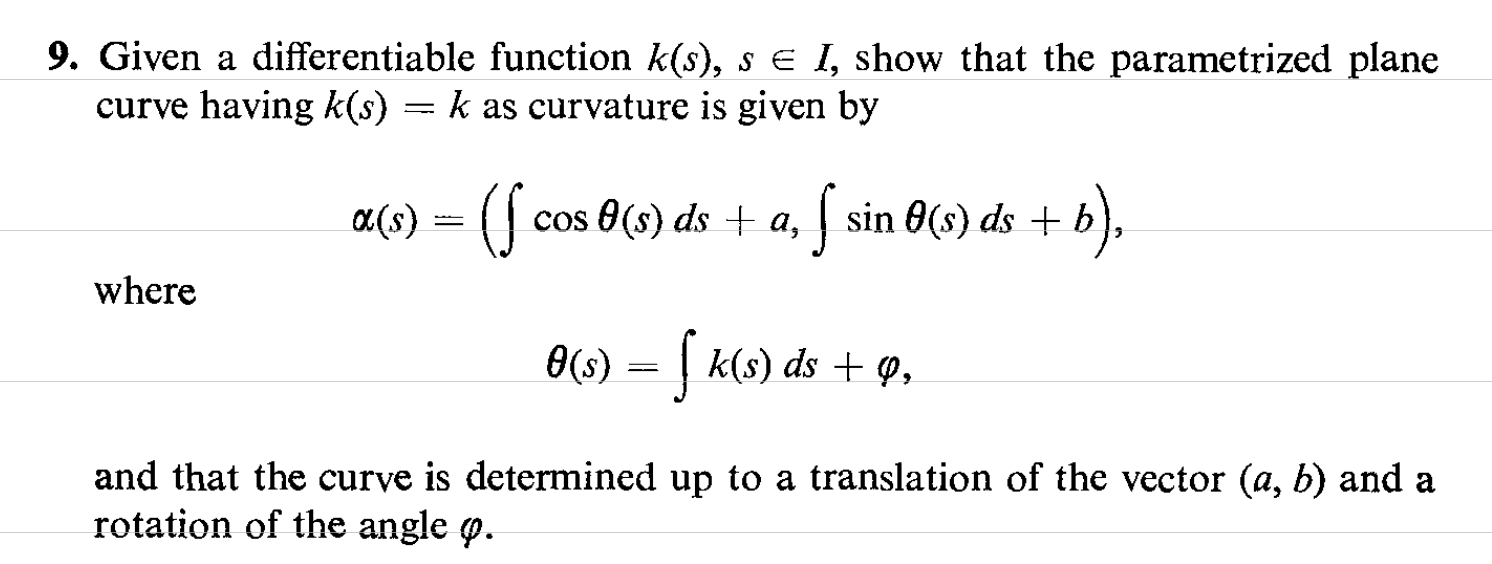
\includegraphics[height=6cm,width=18cm]{hw2q18}
\end{question}
\begin{proof}
By Fundamental Theorem of Local Curves (you can think of our application as identifying $\tau=0$), we know if such curve exists then it is unique up to translation and rotation. This reduced our proof into showing 
\begin{align*}
\vi{\alpha \text{ has curvature $\kappa$ }}
\end{align*}
Compute 
\begin{align*}
\alpha '=(\cos \theta, \sin \theta)
\end{align*}
This shows that $\alpha $ is parametrized by arc-length, and shows that we can compute
\begin{align*}
\abso{\alpha ''}&=\abso{\theta ' (- \sin \theta, \cos \theta)}\\
&=\abso{\theta'}=\abso{\kappa}=\kappa \vdone
\end{align*}
\end{proof}
\begin{question}{}{}
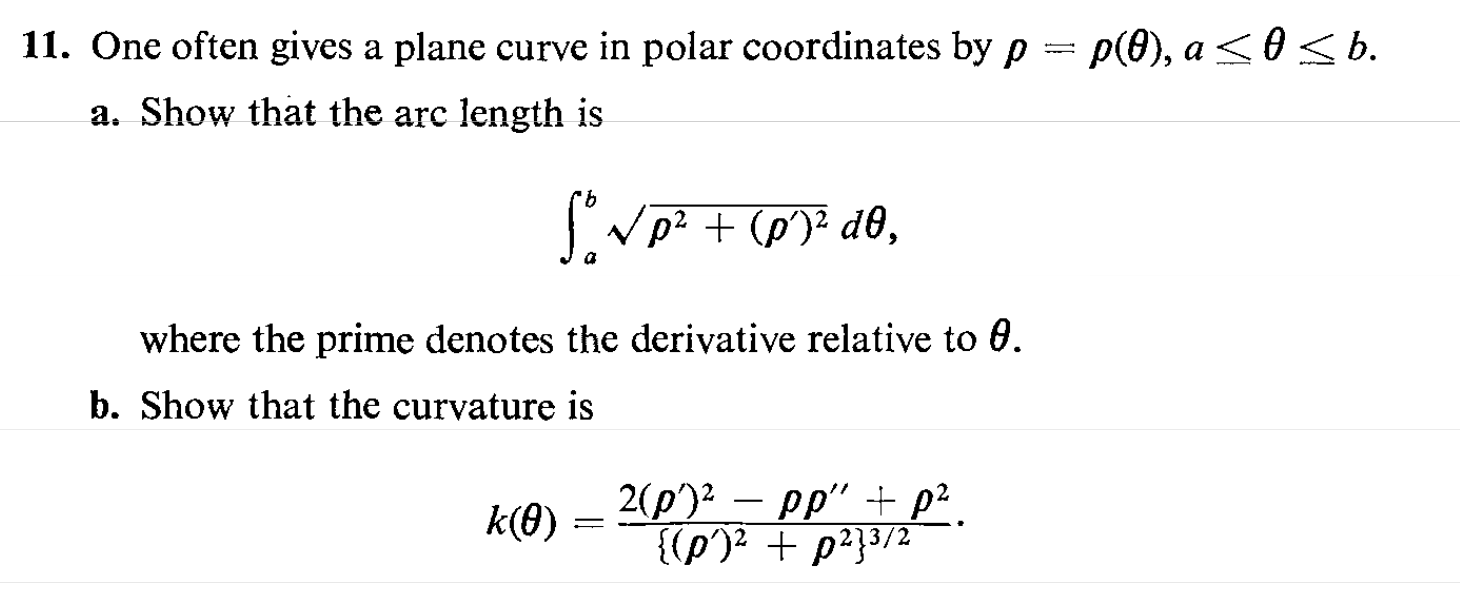
\includegraphics[height=6cm,width=18cm]{hw2q17}
\end{question}
\begin{proof}
\textbf{(a)}

Parametrize by 
\begin{align*}
  \alpha (\theta)\triangleq (x,y)\triangleq (r \cos \theta, r \sin \theta)
\end{align*}
where $r(\theta)$ is a function. With respect to $\theta$, we compute 
\begin{align*}
  (x')^2+(y')^2&=(r'\cos \theta-r\sin \theta)^2+(r' \sin \theta + r \cos \theta)^2\\
  &=(r')^2 \cos ^2 \theta + r^2 \sin ^2 \theta + (r')^2 \sin ^2 \theta + r^2 \cos ^2 \theta \hspace{1cm}(\because \text{ elimination })\\
  &=r^2+(r')^2 
\end{align*}
We now see that the arc-length can be computed by 
\begin{align*}
\int_a^b \abso{\alpha '(\theta)}d\theta&= \int_a^b \sqrt{(x')^2+(y')^2}d\theta \\
&=\int_a^b \sqrt{r^2 +(r')^2}d\theta 
\end{align*}

\textbf{(b)}\\

Recall that 
\begin{align*}
\kappa(t) = \frac{x'y''-x''y'}{\big((x')^2 + (y')^2 \big)^{\frac{3}{2}}}
\end{align*}
plugin 
\begin{align*}
  (x',y')&=(r'\cos \theta -r \sin \theta, r' \sin \theta + r \cos \theta)\\
  (x'',y'')&=(r''\cos \theta -2r' \sin \theta -r\cos \theta, r'' \sin \theta + 2r' \cos \theta  -r \sin \theta)
\end{align*}
To compute 
\begin{align*}
x'y''&= r'r''\cos \theta \sin \theta + 2(r')^2 \cos ^2 \theta -rr'\cos \theta \sin \theta -r r'' \sin ^2 \theta -2rr' \cos \theta \sin \theta +r^2 \sin ^2 \theta\\
x''y'&=r'r''\sin \theta \cos \theta - 2(r')^2 \sin ^2 \theta -rr' \cos \theta \sin \theta +rr'' \cos ^2 \theta - 2rr' \cos \theta \sin \theta  -r^2 \cos ^2 \theta
\end{align*}
Eliminating the odd terms and using $\cos^2+\sin^2=1$, we now compute 
\begin{align*}
\kappa&=\frac{x'y''-x''y'}{\big((x')^2 +(y')^2\big)^{\frac{3}{2}}}\\
&=\frac{2(r')^2-2rr''+r^2}{\big(r^2+(r')^2 \big)^{\frac{3}{2}}}
\end{align*}
\end{proof}

\begin{question}{}{}
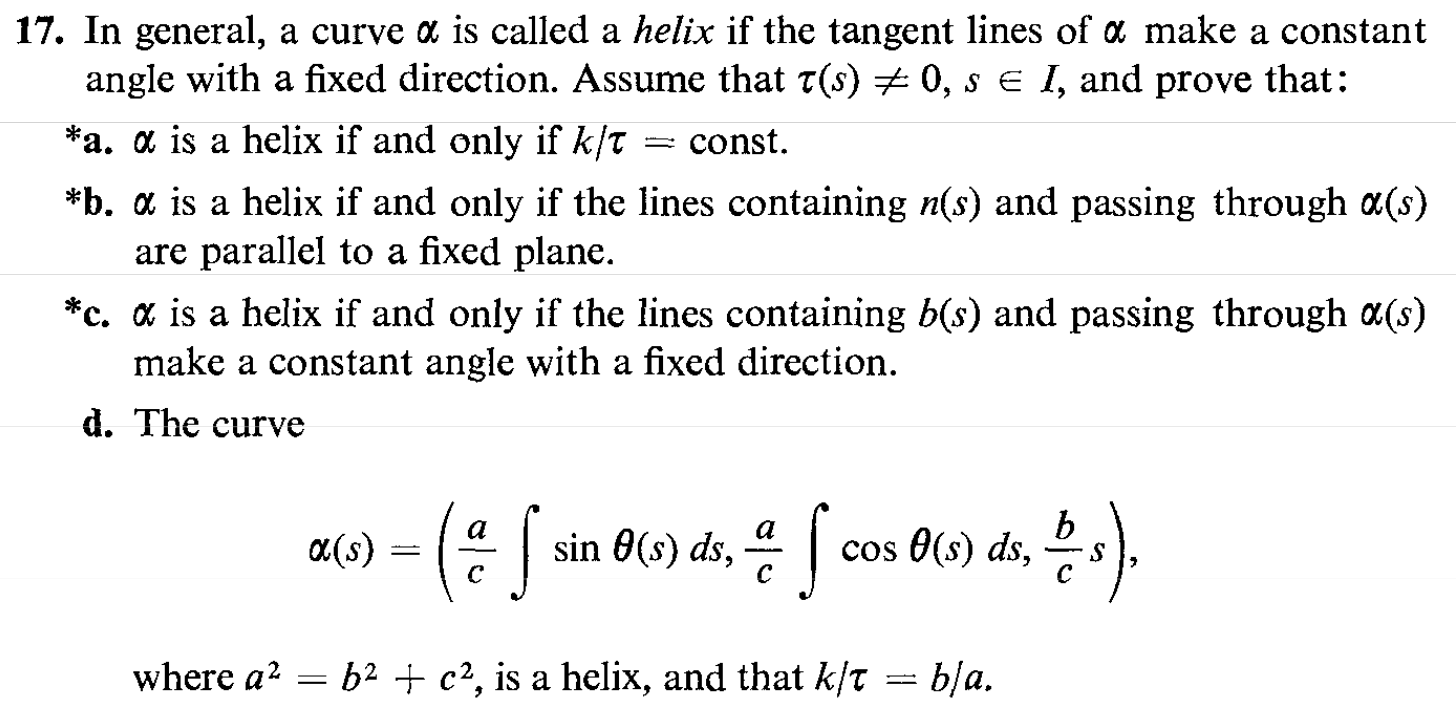
\includegraphics[height=8cm,width=18cm]{hw2q16}
\end{question}
\begin{proof}
\textbf{(a)}
$(\longrightarrow)$\\

Because $\alpha $ is a helix, we know there exists fixed unit $a \inr^3$ and $b \inr$ such that 
\begin{align*}
\alpha '  \cdot a =b \text{ for all $s$ }
\end{align*}
This then implies 
\begin{align*}
\alpha '' \cdot a = 0\text{ for all $s$ }
\end{align*}
which implies 
\begin{align*}
N\cdot a =0
\end{align*}
since $N$ is parallel with  $\alpha ''$. Because $\set{T,N,B}$ is an orthonormal basis, this $(N\cdot a =0)$ together with $a$ being unit then tell us we can express $a$ by
\begin{align*}
a= T \cos \theta + B \sin \theta \text{ for some fixed $\theta \inr$ }
\end{align*}
We now have the information $T \cos \theta + B \sin \theta$ is a constant function  in $s$. Then, using Frenet Formula, we can deduce 
\begin{align*}
  0=(T \cos \theta + B \sin \theta)'&= \kappa N \cos \theta + \tau N \sin \theta
\end{align*}
This them implies 
\begin{align*}
\frac{\kappa}{\tau}=\frac{-\sin \theta}{\cos \theta}\text{ is a constant since $\theta $ is fixed. }
\end{align*}
Notice that $\cos \theta \neq 0$ because $\tau \neq 0$ for all $s$.\\

$(\longleftarrow)$\\

Define $\theta\inr$ by 
\begin{align*}
\theta=\arctan \frac{-\kappa}{\tau}
\end{align*}
We wish to show 
\begin{align*}
  \vi{a=T \cos \theta + B \sin \theta \text{ suffice }}
\end{align*}
Because we have 
 \begin{align*}
T\cdot a= \cos \theta 
\end{align*}
We only wish to show 
\begin{align*}
  \vi{a\text{ is a constant function in $s$ }}
\end{align*}
Because $\theta=\arctan \frac{-\kappa}{\tau}$, we know 
\begin{align*}
\frac{\sin \theta}{\cos \theta}=\tan \theta = \frac{-\kappa}{\tau}
\end{align*}
This then tell us 
\begin{align*}
\tau \sin \theta + \kappa \cos \theta =0
\end{align*}
and implies 
\begin{align*}
\tau N \sin \theta + \kappa N \cos \theta =0
\end{align*}
Then 
\begin{align*}
a'&=(T\cos \theta+ N \sin \theta)'\\
&= \kappa N \cos \theta + \tau N \sin \theta =0 
\end{align*}
This implies $a$ is indeed a constant.  $\vdone$\\

\textbf{(b)}\\

$(\longrightarrow)$\\

Let $a\inr^3$ be the unit vector such that 
\begin{align*}
T\cdot a \text{ is fixed }
\end{align*}
We now see 
\begin{align*}
N\cdot a= (T\cdot a)'=0
\end{align*}
This implies 
\begin{align*}
\text{ the plane $\set{a}^{\perp}$ suffice }
\end{align*}

$(\longleftarrow)$\\

Observe that 
\begin{align*}
&0=N \cdot a= \frac{T'}{\abso{T'}} \cdot a \\
&\implies T' \cdot a =0\\
&\implies T\cdot a\text{ is fixed }
\end{align*}

\textbf{(c)}\\

$(\longrightarrow)$\\

Because $T \cdot a $ is fixed, we can deduce
\begin{align*}
\kappa N \cdot a =T'\cdot a=0
\end{align*}
Now observe from Frenet Formula that 
\begin{align*}
  (B \cdot a )'=- \tau N \cdot a =0 
\end{align*}
This implies $B \cdot a $ is fixed.\\

$(\longleftarrow)$\\

Because $B \cdot a$ is fixed, we can deduce
\begin{align*}
  &0= (B \cdot a)'=-\tau N \cdot a \\
 &\implies  N \cdot  a=0
\end{align*}
The proof then now follows from the result of  \textbf{(b)}.\\

\textbf{(d)}\\

First we have to notice the fucking typo correction $\frac{\kappa}{\tau}=\frac{a}{b}$.\\

Compute 
\begin{align*}
\alpha '(s)&=\Big(\frac{a}{c}\sin \theta, \frac{a}{c}\cos \theta, \frac{b}{c} \Big)\\
\alpha ''(s)&=\Big(\theta ' \frac{a}{c}\cos \theta , \theta ' \frac{-a}{c}\sin \theta, 0 \Big)\\
\alpha '''(s)&=\Big(\theta'' \frac{a}{c}\cos \theta + (\theta')^2 \frac{-a}{c}\sin \theta , \theta '' \frac{-a}{c}\sin \theta + (\theta ')^2 \frac{-a}{c}\cos \theta, 0 \Big)
\end{align*}
This give us 
\begin{align*}
&\alpha ' \times \alpha '' \cdot \alpha '''\\
&=\frac{b}{c}\Big[\theta ' \theta '' \frac{-a^2}{c^2}\cos \theta \sin \theta + (\theta ')^3 \frac{-a^2}{c^2}\cos ^2 \theta - \theta' \theta '' \frac{-a^2}{c}\sin \theta \cos \theta - (\theta ')^3 \frac{a^2}{c^2}\sin ^2 \theta \Big]\\
&=\frac{b}{c}\Big( (\theta ')^3 \frac{-a^2}{c^2} \Big)=\frac{-a^2b}{c^3}(\theta ')^3
\end{align*}
And give us 
\begin{align*}
\kappa = \theta' \frac{a}{c}
\end{align*}
We now compute 
\begin{align*}
\frac{\kappa}{\tau}&= \frac{\kappa}{-\frac{\alpha ' \times \alpha '' \cdot \alpha '''}{\kappa ^2}}\\
&=\frac{-\kappa ^3}{\alpha ' \times \alpha '' \cdot \alpha '''}\\
&=\frac{-(\theta')^3 \frac{a^3}{c^3}}{\frac{-a^2b}{c^3}(\theta ')^3}=\frac{a}{b}
\end{align*}



\end{proof}

\begin{question}{}{}
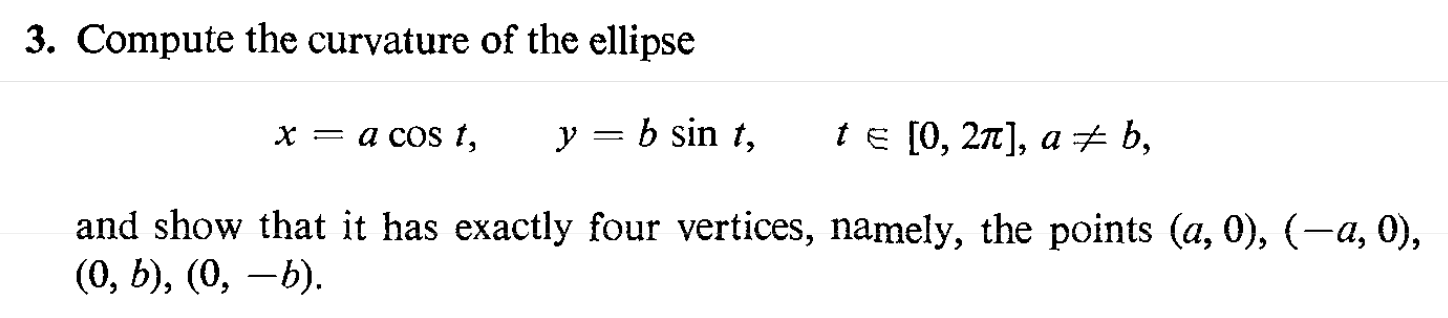
\includegraphics[height=4cm,width=18cm]{hw2q15}
\end{question}
\begin{proof}
Compute 
\begin{align*}
\begin{cases}
  x'=-a \sin t \text{ and }x''=-a\cos t\\
  y'=b \cos t \text{ and } y''=-b \sin t
\end{cases}
\end{align*}
Plugging the curvature formula 
\begin{align*}
\kappa =\frac{x'y''-x''y'}{\big((x')^2 +(y')^2 \big)^{\frac{3}{2}}}
\end{align*}
We now have 
\begin{align*}
\kappa = \frac{ab }{\big(a^2 \sin ^2 t + b^2 \cos ^2 t \big)^{\frac{3}{2}}}
\end{align*}
Compute 
\begin{align*}
\kappa' = (2a^2 \sin t \cos t -2b^2 \sin t \cos t)(a^2\sin ^2 t + b^2 \cos ^2 t)^{\frac{-5}{2}}\cdot (ab)
\end{align*}
We see that 
\begin{align*}
\kappa'=0 \iff  \sin 2t =0
\end{align*}
This only happens when $t \in \set{0,\frac{\pi}{2},\pi,\frac{3\pi}{2},2\pi}$ where $2 \pi$ is just $0$ in the sense of parametrizeation of closed curve. We have shown there are exactly four vertices 
 \begin{align*}
   (a,0),(-a,0),(0,b),(0,-b)
\end{align*}
\end{proof}


\begin{question}{}{}
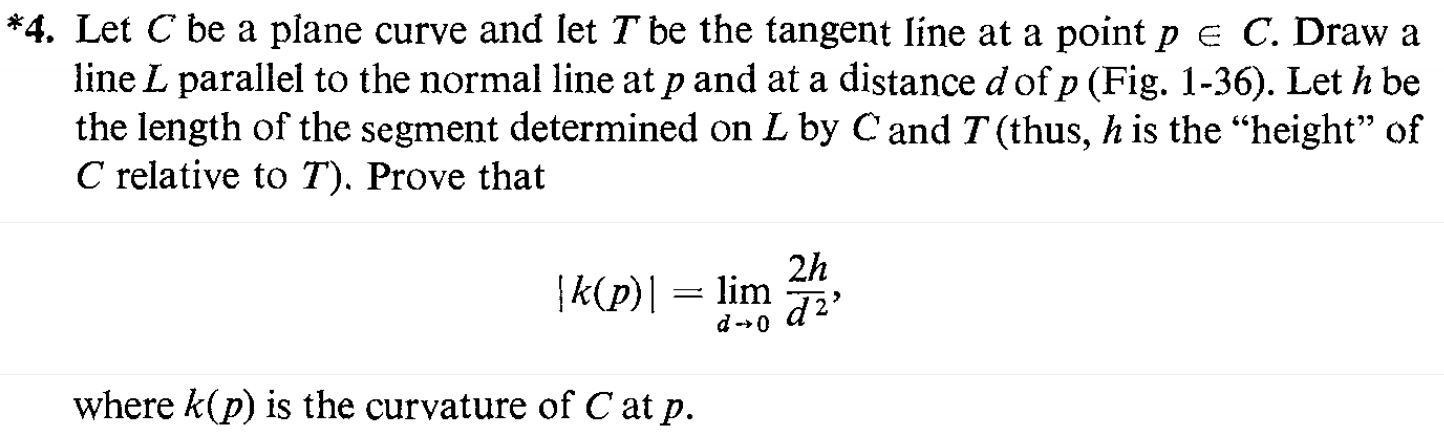
\includegraphics[height=6cm,width=18cm]{hw2q14}
\end{question}
\begin{proof}
WOLG, let $p=(0,0)$, $T$ be the $x$-axis and some neighborhood around $p$ be above  $T$. Positively oriented  parametrize $C$ by arc-length using  $(x,y)$ and $(x,y)(0)=(0,0)$. Using Taylor Theorem about $y(0)$, we see 
\begin{align*}
y(s)=y(0)+y'(0)s + \frac{y''(0)}{2}s^2 + R_y\text{ where $\frac{R_y}{s^2}\to 0$ as $s\to 0$ }
\end{align*}
 Because $T$ the tangent is the $x$-axis, we know $x''(0)=0\hspace{0.5cm}(\because N=(0,1))$. This tell us 
 \begin{align*}
\abso{\kappa(0)}&=\sqrt{(x'')^2(0)+(y'')^2(0)} \\
 &=y''(0)\hspace{1cm}(\because N=(0,1) )
 \end{align*}
\end{proof} 
By our setting $(x,y)(0)=(0,0)$, we see 
\begin{align*}
\hspace{3cm}y(0)=y'(0)=0\hspace{1cm}(\because (x',y')=(1,0))
\end{align*}
We now see 
\begin{align*}
y''(0)= \frac{2\big(y(s)-R_y \big)}{s^2}\text{ for all $s\neq 0$ }
\end{align*}
This tell us 
\begin{align*}
y''(0)=\lim_{s\to 0}\frac{2\big(y(s)-R_y \big)}{s^2}=\lim_{s\to 0}\frac{2y(s)}{s^2}
\end{align*}
Using Taylor Theorem about $x(0)$, we see 
\begin{align*}
x(s)=x(0)+x'(0)s + R_x\text{ where }\frac{R_x}{s}\to 0\text{ as $x \to 0$ }
\end{align*}
Because $x(0)=0$ and $x'(0)=1$, we see 
\begin{align*}
\lim_{s\to 0}\frac{x(s)}{s}=\lim_{s\to 0} \frac{s+R_x}{s}=1
\end{align*}
This now give us 
\begin{align*}
\abso{\kappa (0)}=y''(0)=\lim_{s\to 0}\frac{2y(s)}{s^2}=\lim_{s\to 0}\frac{2y(s)}{x^2(s)}=\lim_{d\to 0}\frac{2h}{d^2}
\end{align*}



\begin{question}{}{}
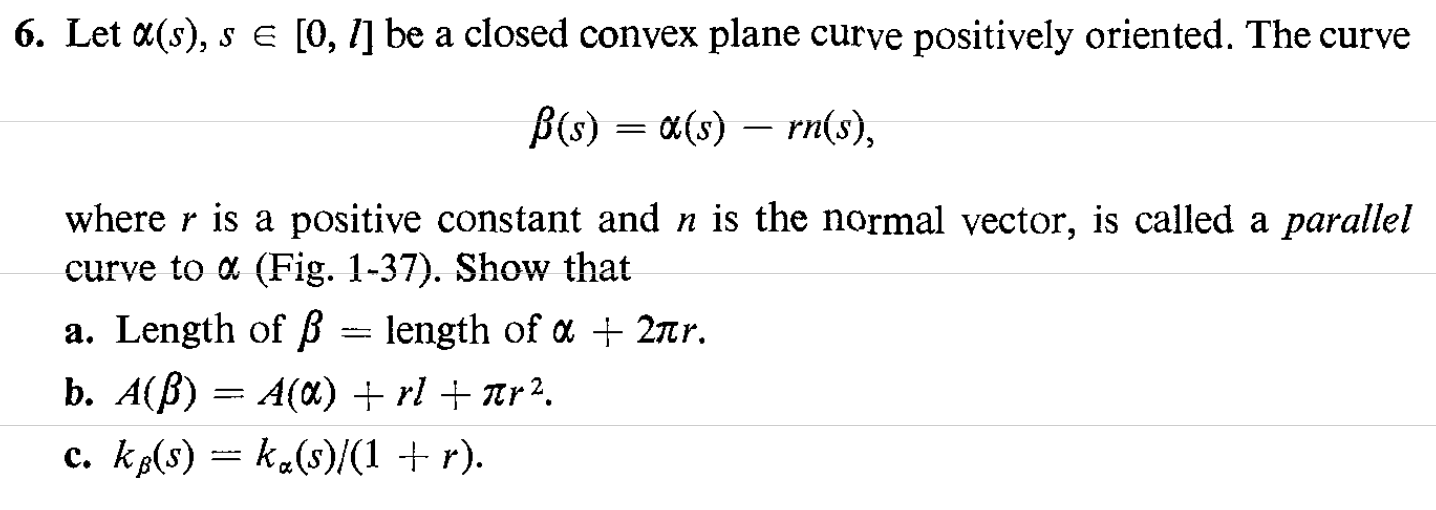
\includegraphics[height=8cm,width=18cm]{hw2q13}
\end{question}
\begin{proof}
\textbf{(a)}\\

Using Frenet Formula to compute 
\begin{align*}
\beta '(s)=\alpha '(s)+r\kappa  T(s)
\end{align*}
Because $\alpha $ is parametrized by arc-length, we now know 
\begin{align*}
  \abso{\beta '}=\abso{(1+r\kappa)\alpha '}=\abso{1+r\kappa }=1+ r\kappa
\end{align*}
This now give us 
\begin{align*}
  \int_0^l \abso{\beta '} ds= l + r \int_0^l \kappa ds
\end{align*}
Because a closed convex curve must also be simple (Sec. 5-7, Prop. 1), we now can deduce 
\begin{align*}
\text{ Length of  }\beta &=l + r \int_0^l \kappa ds\\
&=\text{ Length of }\alpha +r(2\pi)
\end{align*}

\textbf{(b)}\\

Set 
\begin{align*}
\alpha =(x,y)\text{ and }\beta =(x-r N_1,y-rN_2)
\end{align*}
Because 
\begin{align*}
\beta '=(1+ r\kappa)\alpha ' 
\end{align*}
We know 
\begin{align*}
\beta ' =\Big((1+r\kappa)x',(1+r\kappa)y' \Big)
\end{align*}
Now, we use Green's Theorem to compute the Area 
\begin{align*}
A(\beta )&=\frac{1}{2}\int_0^l (x-rN_1)(1+r\kappa)y' -(y-rN_2)(1+r\kappa)x'ds\\
         &=\frac{1}{2}\int_0^l (xy'-yx') ds + \frac{r}{2}\int_0^l (\kappa xy' + \kappa x'y) ds \\
&+ \frac{r}{2}\int_0^l -(N_1y'+N_2x')ds + \frac{r^2}{2}\int_0^l (-N_1y'\kappa+N_2x'\kappa)ds
\end{align*}
Notice that by Frenet Formula, we have
\begin{align*}
N'=- \kappa (x',y')
\end{align*}
so in fact we know 
\begin{align*}
\kappa xy'+\kappa x'y=N'\cdot (-y,x)
\end{align*}
Now using integral by part and the fact $\alpha =(x,y)$ is closed, we know  
\begin{align*}
\int_0^l (\kappa xy'+\kappa x'y)ds&=\int_0^l N' \cdot (-y,x)ds\\
&=\int_0^l N\cdot (-y',x')ds
\end{align*}
Then now we have 
\begin{align*}
  \frac{r}{2}\int_0^l (\kappa xy'+\kappa x'y)ds+\frac{r}{2}\int_0^l -N_1y'+N_2x'ds&=\frac{r}{2}\int_0^l 2N\cdot (-y',x')ds
\end{align*}
Using positive orientation and the fact $\abso{N}=1=\abso{(-y',x')}$ to identify that $N=(-y',x')$, we now have 
\begin{align*}
\frac{r}{2}\int_0^l 2N \cdot (-y',x')ds=rl
\end{align*}
and have 
\begin{align*}
\frac{r^2}{2}\int_0^l (-N_1y'\kappa+N_2x' \kappa)ds=\frac{r^2}{2}\int_0^l \kappa ds =r^2 \pi 
\end{align*}
since $(x,y)$ is simple closed. This finishes the proof. \\

\textbf{(c)}\\

Recall that 
\begin{align*}
\kappa (a,b) = \frac{a'b''-a''b'}{\big((a')^2+(b')^2 \big)^{\frac{3}{2}}}
\end{align*}
We use this formula on $\beta$ to compute
\begin{align*}
\kappa_\beta &= \frac{(1+r\kappa)x'\big((1+r\kappa)y' \big)'-\big((1+r\kappa)x' \big)'(1+r\kappa)y'}{(1+r\kappa)^3}\\
&=\frac{(1+r\kappa)^2 (x'y''-x''y')}{(1+r\kappa)^3}\\
&=\frac{x'y''-x''y'}{1+r \kappa}=\frac{\kappa}{1+r\kappa}\hspace{1cm}(\because (x')^2+(y')^2=1)
\end{align*}
\end{proof}


\begin{question}{}{}
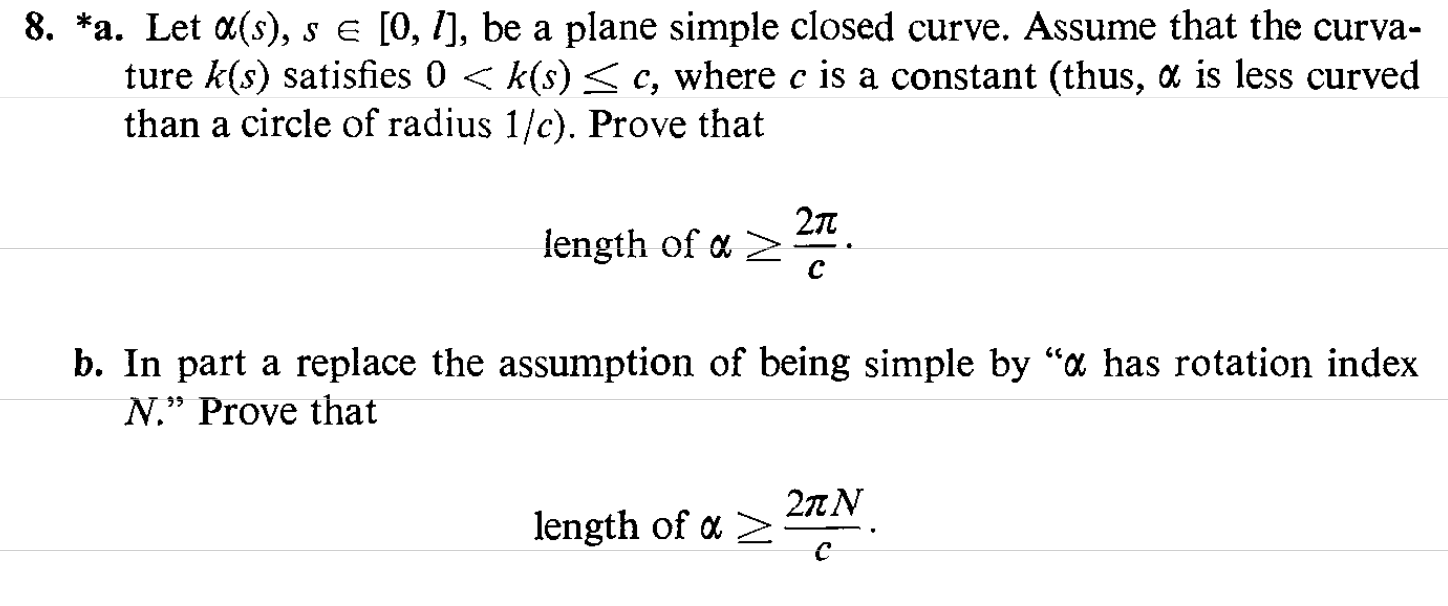
\includegraphics[height=6cm,width=18cm]{hw2q12}
\end{question}
\begin{proof}
\textbf{(a)}\\

Because $\alpha $ is simple closed and $\kappa \leq c$, we know 
\begin{align*}
cl=\int_0^l cds\geq \int_0^l \kappa ds=2\pi
\end{align*}
This then implies 
\begin{align*}
\text{ Length of }\alpha =l\geq \frac{2\pi }{c}
\end{align*}
\textbf{(b)}\\

Because $\alpha $ has rotation index $N$ and  $\kappa \leq c$, we know 
\begin{align*}
cl=\int_0^l cds\geq \int_0^l \kappa ds=N2\pi
\end{align*}
This the implies
\begin{align*}
\text{ Length of }\alpha =l\geq \frac{2\pi N}{c}
\end{align*}
\end{proof}
\begin{question}{}{}
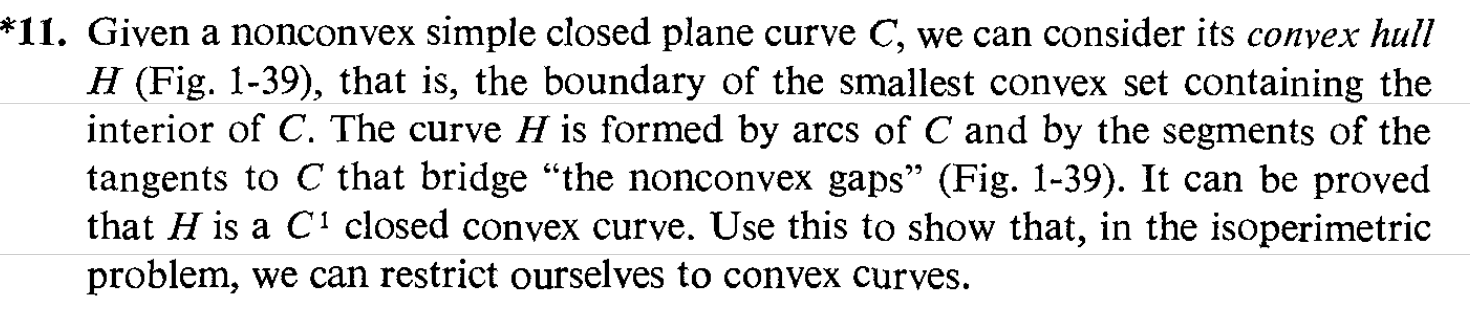
\includegraphics[height=4cm,width=18cm]{hw2q11}

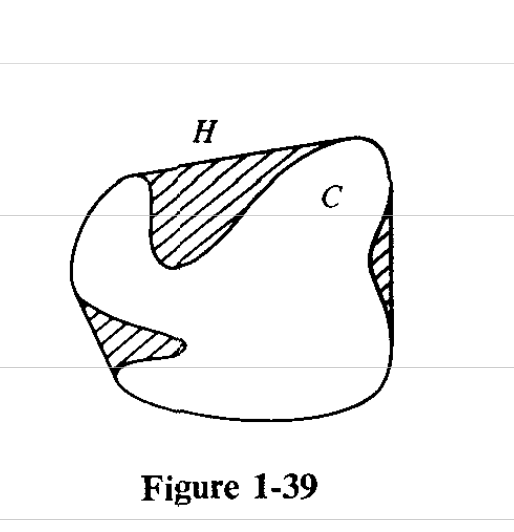
\includegraphics[height=4cm,width=18cm]{hw2q10}
\end{question}
\begin{proof}
Suppose we have proved that a convex closed curve must satisfy the isoperimetric inequality. Let $C$ be an arbitrary closed plane curve, and let  $H$ be its convex hull. Now, because straight line is the shortest curve between two point and because we know $H$, a convex curve, must satisfy isoperimetric inequality, we now see 
 \begin{align*}
4 \pi A(C)\leq 4 \pi A(H)\leq l_H^2 \leq l_C^2
\end{align*}
If the equality hold true, we can deduce from $l_H=l_C$ that  $H=C$ and use the argument for isoperimetric inequality of convex curve to argue that $C=H$ must be a circle.
\end{proof}
\begin{question}{}{}
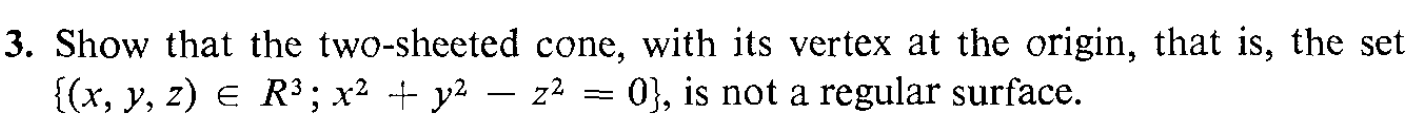
\includegraphics[height=2cm,width=18cm]{hw2q9}
\end{question}
\begin{proof}
Let $S=\set{(x,y,z)\inr^3:x^2+y^2-z^2=0}$. It is clear $S$ contain  $(0,0,0)$. To show $S$ is not regular, we only wish to find a neighborhood $V$ around  $(0,0,0)$ in $S$ such that  $V$ can not expressed as graph of differentiable functions from $\R^2$ to  $\R$. This is trivially true, as all neighborhood ought to contain some open ball $B_\epsilon (0)$, and in this open ball, if we fix, say $(x,y)\in B_\epsilon (0)$ such that $(x,y,\sqrt{x^2+y^2}) \in B_\epsilon (0)$, we see that $z=-\sqrt{x^2+y^2} $ is also in $B_\epsilon (0)$ and $S$. The same argument applies to when $(x,z)$ and $(y,z)$ are fixed. 
\end{proof}
\begin{question}{}{}
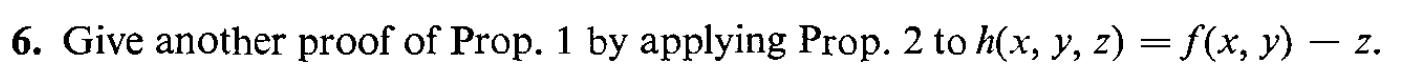
\includegraphics[height=1cm,width=18cm]{hw2q8}
\end{question}
\begin{proof}
Because $f$ is differentiable, we see $f_x,f_y$ are all continuous on $U$. This then implies 
 \begin{align*}
h_x(x,y,z)=f_x(x,y),h_y(x,y,z)=f_y(x,y),h_z=-1\text{ are all continuous on $U$ }
\end{align*}
We have shown $h$ is differentiable. Now that observe 
\begin{align*}
h(x,y,z)=0 \implies (x,y,z)=(x,y,f(x,y))
\end{align*}
The converse of course hold true. This then implies 
\begin{align*}
  f[U]=h^{-1}[0]
\end{align*}
Fix arbitrary $(x,y) \in U$. We see 
 \begin{align*}
\textbf{d}h\big(x,y,f(x,y) \big)=\begin{bmatrix} 
  h_x & h_y & h_z
\end{bmatrix}\Big|_{(x,y,f(x,y))}=\begin{bmatrix}
  f_x(x,y) & f_y(x,y) & -1 
\end{bmatrix}
\end{align*}
which is clearly not onto. This show 
\begin{align*}
  (x,y,f(x,y))\text{ is not a critical point }
\end{align*}
Because $(x,y) \in U $ is arbitrary, we have shown $f[U]$ contain no critical point. Now it follows $0$ is a regular value and $f[U]=h^{-1}[0]$ is a regular surface.
\end{proof}
\begin{question}{}{}
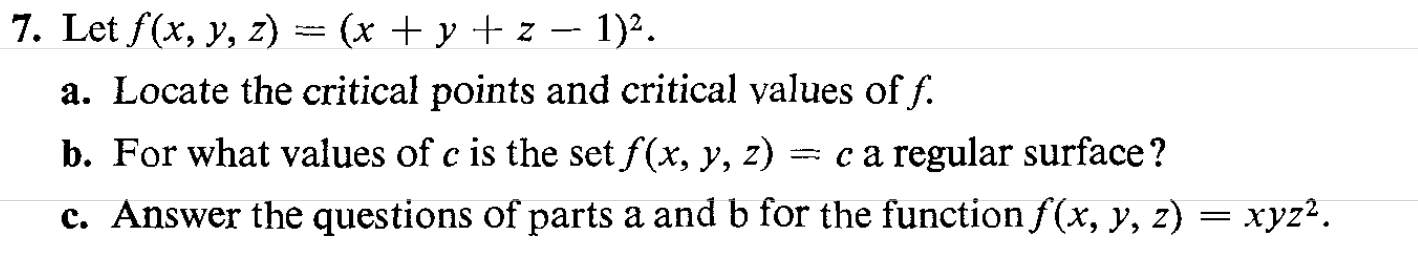
\includegraphics[height=3cm,width=18cm]{hw2q7}
\end{question}
\begin{proof}
\textbf{(a)}\\

Compute 
\begin{align*}
f_x=f_y=f_z=2(x+y+z-1)
\end{align*}
This implies the set of critical points are 
\begin{align*}
\set{(x,y,z)\inr^3:x+y+z=1}
\end{align*}
Then it follows from simple computation the set of  critical values is exactly 
\begin{align*}
\set{0}
\end{align*}
\textbf{(b)}\\

For all $c>0$,  the set $f^{-1}[c]$ is a regular surface, and for all $c<0$, the set  $f^{-1}[c]$ is empty (thus trivially regular).\\

\textbf{(c)}\\

Compute 
\begin{align*}
f_x=yz^2\text{ and }f_y=xz^2\text{ and }f_z=2xyz
\end{align*}
This implies the set of critical points is 
\begin{align*}
\set{(x,y,z):z=0\text{ or }x=y=0}
\end{align*}
With simple computation, we see the set of  critical values is exactly 
\begin{align*}
\set{0}
\end{align*}
The set of regular values are exactly $\R^*$, so all  $c\neq 0$ suffice.
\end{proof}
\begin{question}{}{}
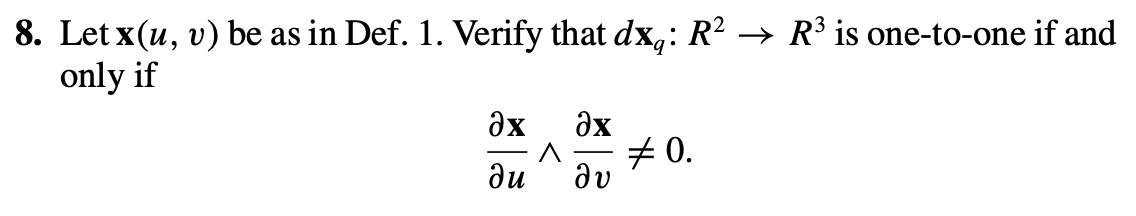
\includegraphics[height=3cm,width=18cm]{Ghw2b}
\end{question}
\begin{proof}
Note that 
\begin{align*}
dx_q=\begin{bmatrix}
  \partial_u x & \partial_v x
\end{bmatrix}
\end{align*} 
This give us 
\begin{align*}
dx_q:\R^2 \rightarrow \R^3\text{ is one-to-one }\iff \partial_ux, \partial_vx \inr^3 \text{ is linearly independent everywhere }
\end{align*}
Then we can reduce the problem into proving 
\begin{align*}
\partial _u x, \partial_v x\inr^3 \text{ is linearly independent everywhere }\iff \partial_ux\times\partial_v x\neq 0\text{ everywhere }
\end{align*}
This then follows from \myref{Theorem}{CtcL} at the next page, as one can see that each component of the output of cross product is exactly the three determinant. 
\end{proof}
\begin{theorem}
\label{CtcL}
  \textbf{(Computation to check Linearly Independence)} 
\begin{align*}
\begin{bmatrix}
  v_1 & w_1\\
  v_2 & w_2 \\
  v_3 & w_3
\end{bmatrix}\text{ is linearly independent }\iff \begin{vmatrix} 
  v_1 & w_1\\
  v_2 & w_2
\end{vmatrix}\neq 0\text{ or }\begin{vmatrix} 
  v_2 & w_2\\
  v_3 & w_3
\end{vmatrix}\neq 0\text{ or }\begin{vmatrix} 
  v_1 & w_1\\
  v_3 & w_3
\end{vmatrix}\neq 0
\end{align*}
\end{theorem}
\begin{proof}
$(\longleftarrow)$\\

\As{$v,w$ are linearly dependent}. Fix $w_k=cv_k$. We see 
\begin{align*}
\begin{vmatrix} 
  v_1 & w_1 \\
  v_2 & w_2
\end{vmatrix}=cv_1v_2-cv_1v_2=0\tCaC
\end{align*}

$(\longrightarrow)$\\

\As{all determinant are $0$}. Pick $k$ such that $v_k$ is non-zero. Define 
\begin{align*}
c\triangleq \frac{w_k}{v_k}
\end{align*}
WOLG, suppose 
\begin{align*}
w_1=cv_1\text{ and }v_1\neq 0
\end{align*}
We then can deduce
\begin{align*}
\begin{vmatrix} 
  v_1 & w_1 \\
  v_2 & w_2
\end{vmatrix}\implies cv_1v_2=v_1w_2 \implies w_2=cv_2
\end{align*}
The same arguement implies $w_3=cv_3\tCaC$
\end{proof}
\section{HW3}
\begin{question}{}{}
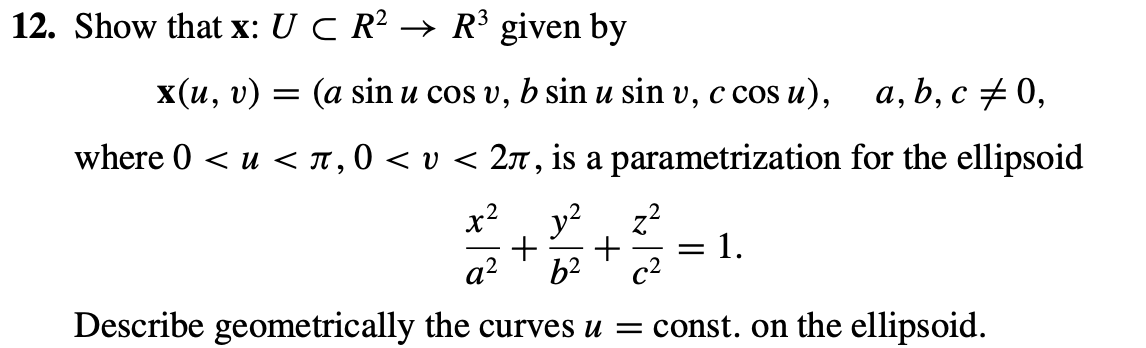
\includegraphics[height=5cm,width=18cm]{HW312}
\end{question}
\begin{proof}
We are required to show 
\begin{enumerate}[label=(\alph*)]
  \item range of $\textbf{x}$ lies in the ellipsoid
  \item $\textbf{x}$ is smooth 
  \item $d\textbf{x}$ is one-to-one everywhere on $U\triangleq (0,\pi)\times (0,2\pi)$ 
  \item $\textbf{x}$ is a homeomorphism
\end{enumerate}
Compute 
\begin{align*}
\frac{x^2}{a^2}+\frac{y^2}{b^2}+\frac{z^2}{c^2}&=\sin^2 u \cos^2 v + \sin^2 u \sin^2 v + \cos^2 u=1
\end{align*}
This shows that the range of  $\textbf{x}$ indeed lies in the ellipsoid.\\

It is clear that $\textbf{x}$ is smooth.\\

Compute 
\begin{align*}
d\textbf{x}=\begin{bmatrix}
  a\cos u \cos v & -a \sin u \sin v\\
  b \cos u \sin v & b \sin u \cos v \\
  -c \sin u & 0 
\end{bmatrix}
\end{align*}
Then compute
\begin{align*}
\frac{\partial (y,z)}{\partial (u,v)}=bc \sin^2 u \cos v\text{ and }\frac{\partial (x,z)}{\partial (u,v)}=-ac \sin^2 u \sin v
\end{align*}
Because $u \in (0,\pi)$ and $v \in (0,2\pi)$, and $b,c\neq 0$, we now can deduce
\begin{align*}
&\frac{\partial (y,z)}{\partial (u,v)}=0\iff v\in \set{\frac{\pi}{2},\frac{3}{2}\pi}\\
&\frac{\partial (y,z)}{\partial (u,v)}=0\iff v=\pi 
\end{align*}
This then let us deduce 
\begin{align*}
d\textbf{x}\text{ is one-to-one everywhere on }(0,\pi)\times (0,2\pi)
\end{align*}
Traditionally, the function $\arctan$ is defined on $\R$ and have codomaiin $(-\frac{\pi}{2},\frac{\pi}{2})$.\\

Deduce first from the $z$-component of  $\textbf{x}$. We see
\begin{align*}
\textbf{x}^{-1}(x,y,z)=
  \Big(\arccos \frac{z}{c}, \begin{cases}
    \arctan \frac{ay}{bx}& \text{ if $x,y\inr^+$ (first quadrant) }\\
    \frac{\pi}{2}& \text{ if $x=0,y\inr^+$ }\\
    \frac{3\pi}{2}+\arctan \frac{ay}{bx}& \text{ if $x\inr^-,y\inr^+$ (second quadrant) }\\
    \pi + \arctan \frac{ay}{bx}& \text{ if $x\inr^-,y\inr^-_0$ (third quadrant) }\\ 
    \frac{3\pi }{2}& \text{ if $x=0,y\inr^-$ }\\
    \frac{4\pi }{2}+\arctan \frac{ay}{bx}& \text{ if $x\inr^+,y\inr^-$ (forth quadrant) }
  \end{cases}\Big)
\end{align*}
Now it follows that $\textbf{x}$ is indeed a homeomorphism.\\

When $u$ is fixed, the image is an oval missing a point $(a\sin u, 0,c \cos u)$ floating in air (contained by $\set{(x,y,c_0)\inr^3:(x,y)\inr^2}$ where $c_0=c \cos u$ is fixed )
\end{proof}
\begin{definition}
\textbf{(Definition of regular plane curve)} We say $C\subseteq \R^2$ is a regular plane curve if for all $p\in  C$ there exists 
\begin{enumerate}[label=(\alph*)]
  \item an open neighborhood $p \in V \subseteq \R^2$ 
  \item an open set $U\subseteq \R$
  \item a function $\textbf{x}:U \rightarrow V\cap C $
\end{enumerate}
such that $\textbf{x}$ satisfy
\begin{enumerate}[label=(\alph*)]
  \item $\textbf{x}$ is smooth 
  \item $\textbf{x}$ is a homoeomorphism between $U$ and  $V\cap C$
  \item $d\textbf{x}_q\in L(\R,\R^2)$ is one-to-one for all $q \in U$
\end{enumerate}
\end{definition}
\begin{definition}
\textbf{(Definition of regular space curve)} We say $C\subseteq \R^3$ is a regular space curve if for all $p\in  C$ there exists 
\begin{enumerate}[label=(\alph*)]
  \item an open neighborhood $p \in V \subseteq \R^3$ 
  \item an open set $U\subseteq \R$
  \item a function $\textbf{x}:U \rightarrow V\cap C $
\end{enumerate}
such that $\textbf{x}$ satisfy
\begin{enumerate}[label=(\alph*)]
  \item $\textbf{x}$ is smooth 
  \item $\textbf{x}$ is a homoeomorphism between $U$ and  $V\cap C$
  \item $d\textbf{x}_q\in L(\R,\R^3)$ is one-to-one for all $q \in U$
\end{enumerate}
\end{definition}
\begin{question}{}{}
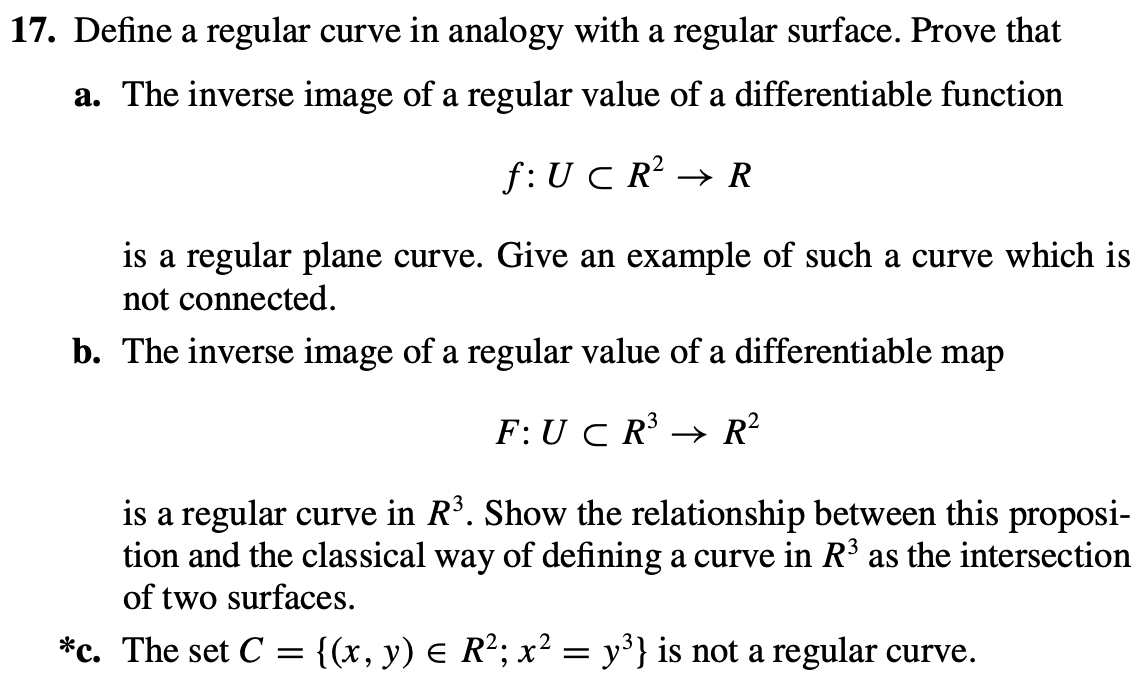
\includegraphics[height=8cm,width=18cm]{HW317}
\end{question}
\begin{proof}
\textbf{(a)}\\

Suppose $f:U\subseteq \R^2\rightarrow \R$ is a smooth function and $c$ is a regular value. We wish to prove 
\begin{align*}
  \vi{C\triangleq f^{-1}[c]\text{ is a regular plane curve }}
\end{align*}
Fix $p \in f^{-1}[c]$. We wish 
\begin{align*}
\vi{\text{ to find a local parametrization $\textbf{x}: I \subseteq \R \rightarrow  C$ around $p$}}
\end{align*}
Because $c$ is a regular value, we know $df_p$ is one-to-one. Then, WOLG, we can let $\partial_y F(p)\neq c$. Define $F:U\rightarrow \R^2$ by 
\begin{align*}
F(x,y)\triangleq \Big(x,f(x,y)\Big)
\end{align*}
Compute 
\begin{align*}
dF=\begin{bmatrix}
  1 & 0 \\
  \partial_x f & \partial _yf 
\end{bmatrix}
\end{align*}
It is now clear that  $\text{det}(dF_p)\neq 0$. Now, because $f$ is smooth, we can use inverse function Theorem and obtain a diffeoemorphism $F$ between open neighborhood around $p$ and open neighborhoood around $f(p)$. Now, note that $f[C]=\set{c}$. This tell us 
\begin{align*}
F[C]\subseteq \set{(x,c)\inr^2:x\inr}
\end{align*}
we now claim
\begin{align*}
 \vi{\textbf{x}(u)\triangleq F^{-1}(u,c)\text{ is the desired local parametrization around $p$ }}
\end{align*}
The fact that $\textbf{x}$ is smooth and homeomorphism follows from 
\begin{enumerate}[label=(\alph*)]
  \item $F$ is a diffeomorphism around $p$ 
  \item $\textbf{x}$ can be identified as restriction of $F^{-1}$
\end{enumerate}
Note that $d(F^{-1})_p=\big(dF_{F^{-1}(p)} \big)^{-1}\neq 0$. Now, because $\textbf{x}$ is restriction of $F^{-1}$, we see $d\textbf{x}$ must not be $0$ around  $p$. $\vdone$ \\

An example is $f(x,y)=(y-1)^2 -x^2$.\\

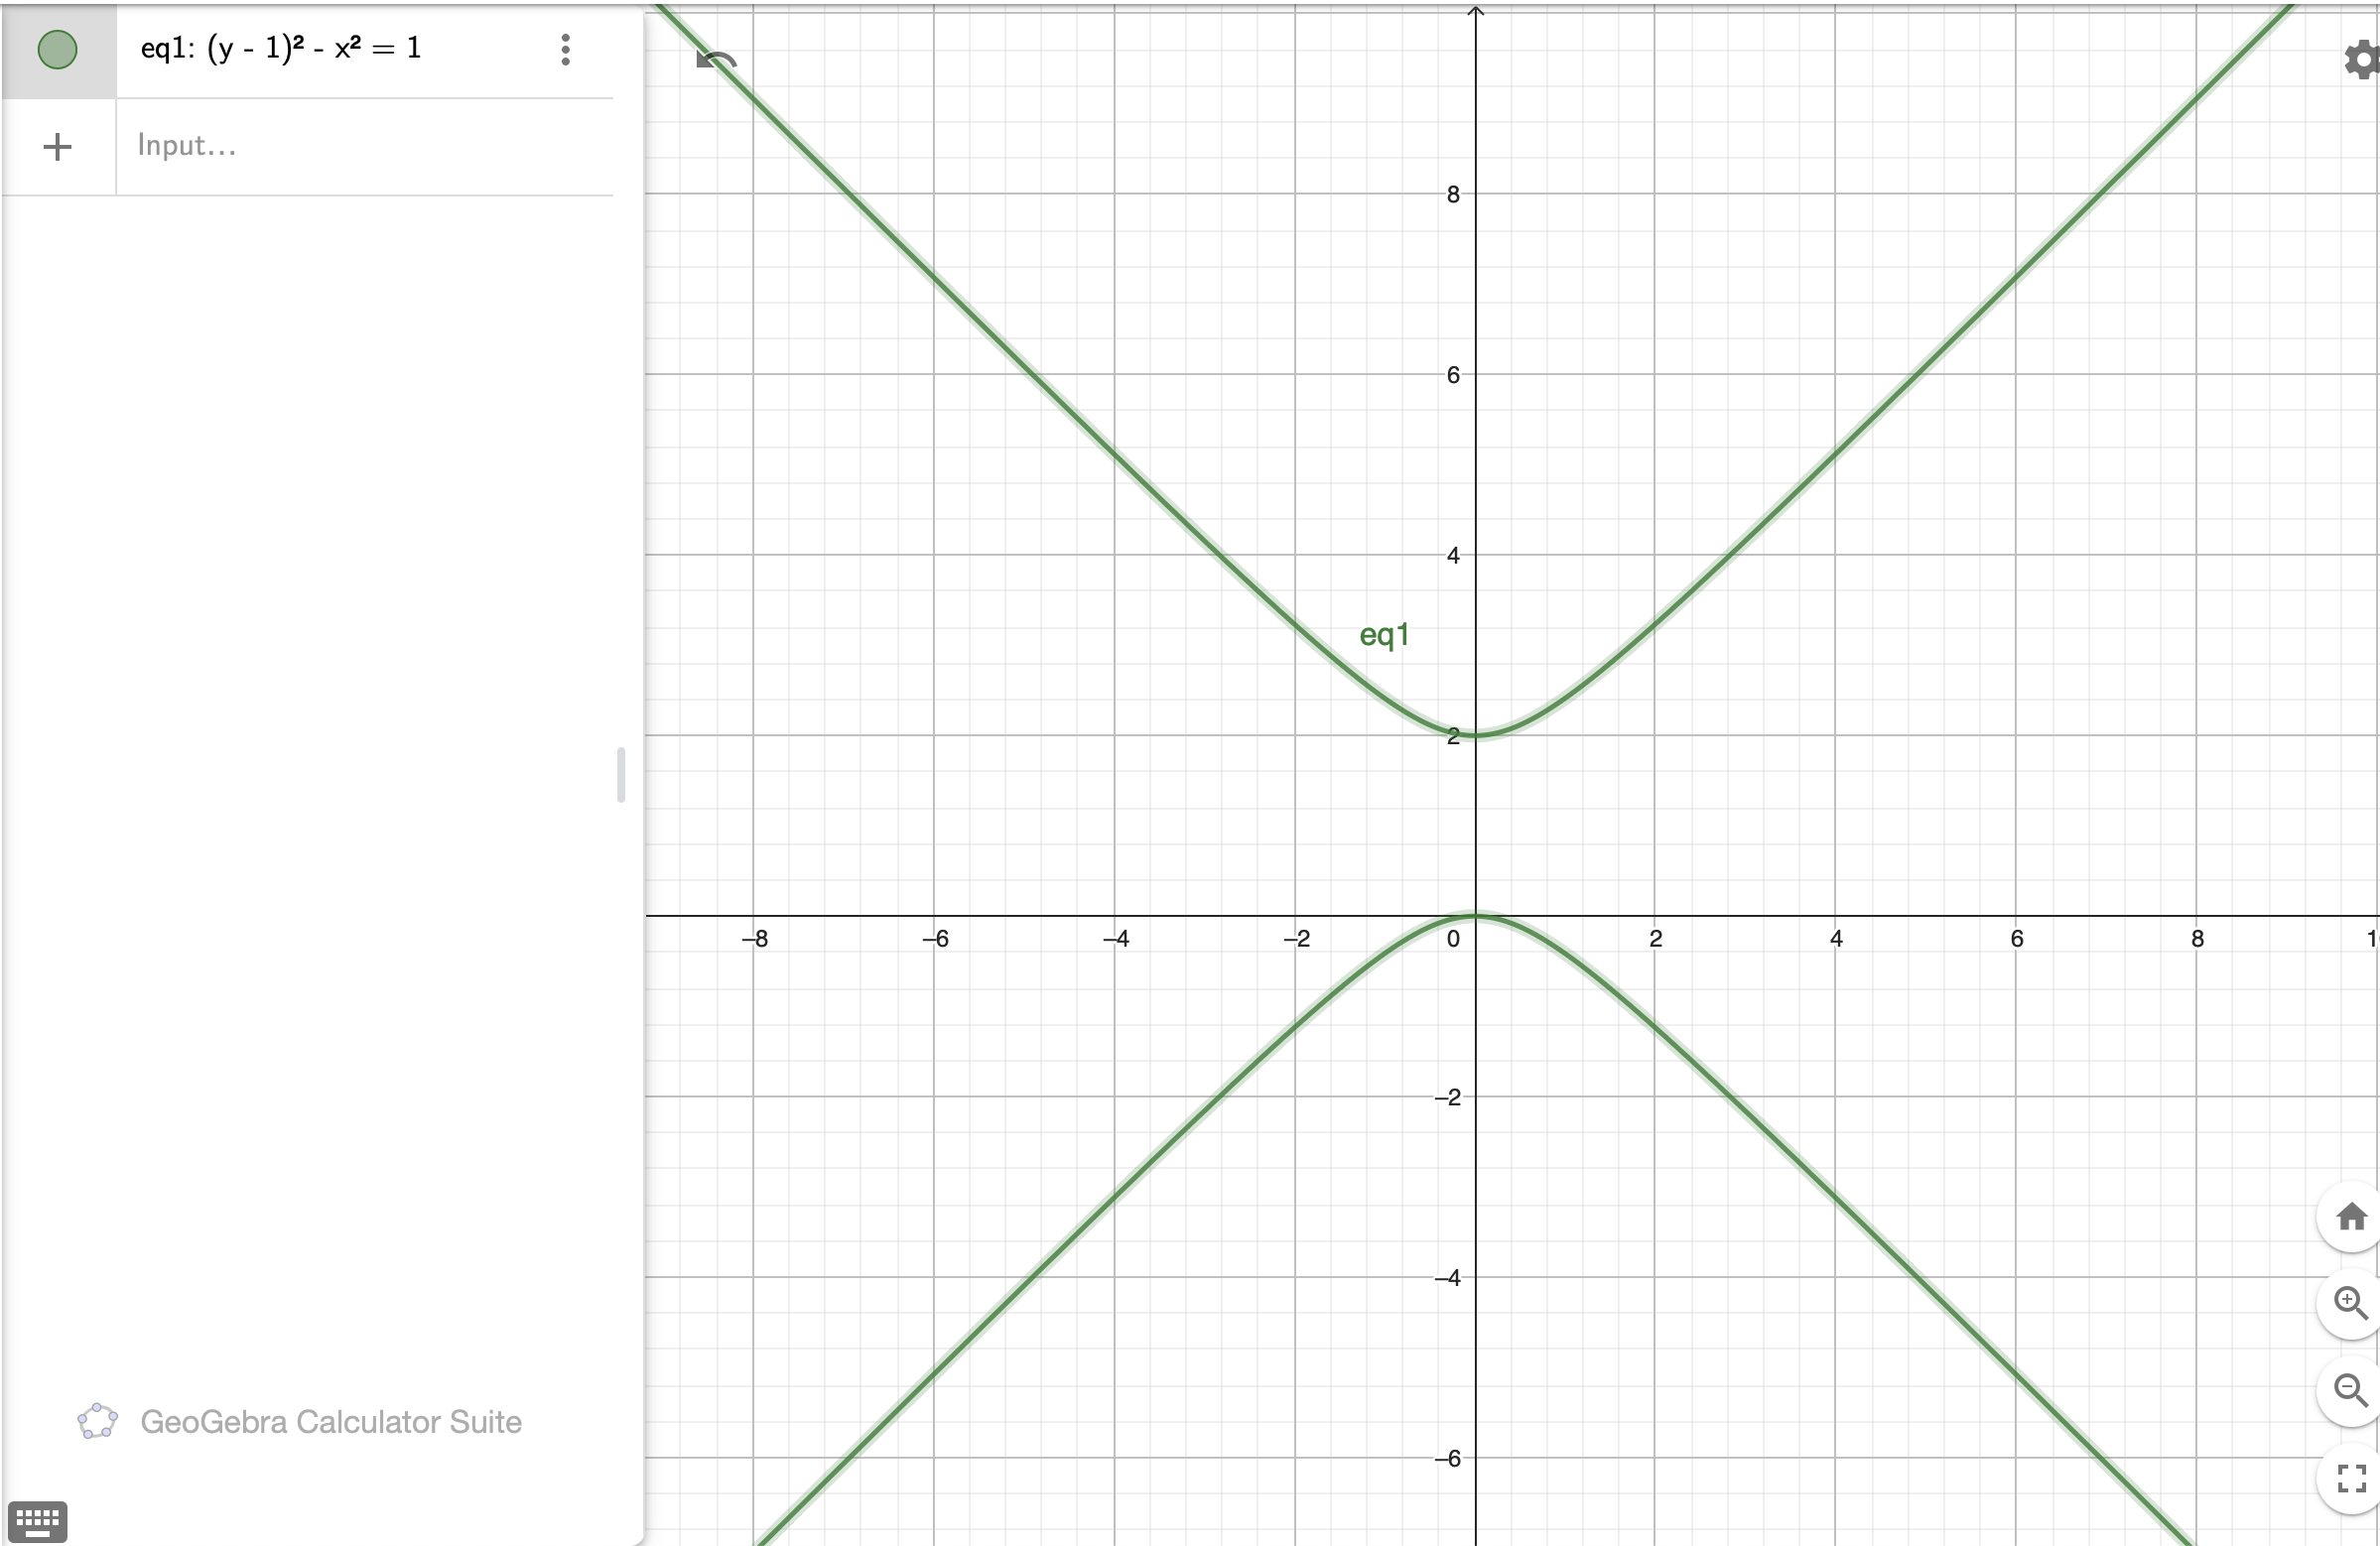
\includegraphics[height=10cm,width=18cm]{HW3pic1}


\textbf{(b)}\\

Suppose $F:U\subseteq \R^3\rightarrow \R^2$ is a smooth function and $(c_0,c_1)$ is a regular value. We wish to prove 
\begin{align*}
\vi{C\triangleq F^{-1}[(c_0,c_1)]\text{ is a regular space curve }}
\end{align*}
Fix $p\in  F^{-1}[(c_0,c_1)]$. We wish 
\begin{align*}
\vi{\text{ to find a local parametrization $\textbf{x}:I\subseteq \R\rightarrow C$  around $p$ }}
\end{align*}
Define $G:U\rightarrow \R^3$ by
\begin{align*}
G(x,y,z)\triangleq \Big(x,F(x,y,z) \Big)
\end{align*}
Compute 
\begin{align*}
dG=\begin{bmatrix}
  1 & 0 & 0 \\
  \partial_x F_1 & \partial_y F_1 & \partial_z F_1\\
  \partial_x F_2 & \partial_y F_2 & \partial_z F_2
\end{bmatrix}
\end{align*}
Because $p$ is a regular point of $F$, we can WOLG, suppose 
\begin{align*}
\text{det}\big( dG_p\big)=\text{det}\Big( \frac{\partial (F_1,F_2)}{\partial (y,z)}\Big|_p\Big)\neq 0
\end{align*}
This Then, by Inverse function Theorem, $G$ is locally a diffeomorphism around $p$. We now see 
\begin{align*}
\textbf{x}(t)\triangleq G^{-1}(t,c_0,c_1)\text{ is the desired local parametrization around $p\vdone$}
\end{align*}
Suppose we are given two function $A,B:\R^3\rightarrow \R$, and suppose  $A^{-1}[c_0],B^{-1}[c_1]$ are two surfaces. Define $F:\R^3\rightarrow \R^2$ by  
\begin{align*}
F(p)\triangleq (A(p),B(p))
\end{align*}
We see that 
\begin{align*}
\text{ the intersection }A^{-1}[c_0]\cap B^{-1}[c_1]\text{ is exactly }F^{-1}[(c_0,c_1)]
\end{align*}

\textbf{(c)}\\

\As{for a contradiction, $C$ is a regular curve}. Note that $(0,0)\in C$. We know there exists an open-neighborhood $N\subseteq \R^2$ around $(0,0)$ such that $N\cap C$ is the graph of some differentiable function in $x$ or  $y$. However, this is impossible, since if one view $N\cap C$ as a function in $x$, the function  $y=x^{\frac{2}{3}}$ is not differetaible at $x=0$, and one can not even view $N\cap C$ as a function in $y$ as each  $y$ correspond to two $x$, namely  $x=\pm y^{\frac{3}{2}}$. $\tCaC$ 

\end{proof}
\begin{question}{}{}
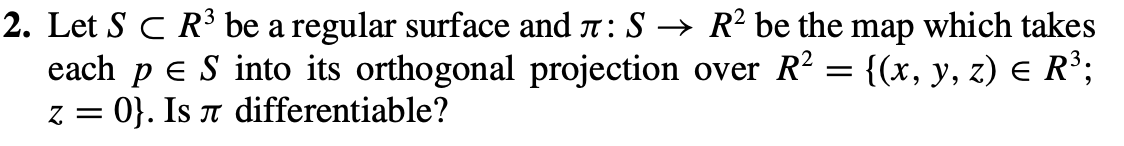
\includegraphics[height=3cm,width=18cm]{HW3a6}
\end{question}
\begin{proof}
Yes. Fix $p$ in  $S$. We wish to prove 
 \begin{align*}
\vi{\pi\text{ is differentiable at $p$ in the sense of manifold }}
\end{align*}
Let $\textbf{x}_1:U_1\subseteq \R^2 \rightarrow V_1 \cap  S\subseteq \R^3$ be a local parametrization around $p$. Define a local parametrization $\textbf{x}_2:U_2 \subseteq \R^2 \rightarrow \R^2 $ around $\pi(p)$ by 
\begin{align*}
\textbf{x}_2\triangleq \textbf{id}_{U_2}
\end{align*}
We are require to prove 
\begin{align*}
  \vi{\textbf{x}_2^{-1}\circ \pi \circ \textbf{x}_1\text{ is differentiable at $\textbf{x}_1^{-1}(p)$ }}
\end{align*}
Notice that 
\begin{enumerate}[label=(\alph*)]
  \item $\textbf{x}_1:U_1 \rightarrow \R^3$ is differentiable at $p$ by definition 
  \item $\pi :\R^3 \rightarrow \R^2$ is clearly differntiable, with derivative $\begin{bmatrix}
      1 & 0 &0 \\
      0 & 1 &0 \\
      0 & 0 &0 
  \end{bmatrix}$
  \item $\textbf{x}_2^{-1}=\textbf{id}_{U_2}:U_2 \rightarrow \R^2$ is clearly differntiable. 
\end{enumerate}
This shows that $\textbf{x}_2^{-1}\circ  \pi \circ  \textbf{x}_1$ is differentiable at $p$. $\vdone$ 
\end{proof}


\begin{question}{}{}
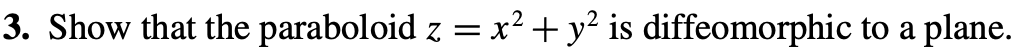
\includegraphics[height=1.5cm,width=18cm]{HW3a5}
\end{question}
\begin{proof}
Let $S$ be the paraboloid. We show 
\begin{align*}
\vi{S\text{ is diffeomorphic to }\set{(x,y,0):x,y\inr}}
\end{align*}
Define 
\begin{align*}
\pi:S\rightarrow \set{(x,y,0):x,y\inr}\text{ by }\pi(x,y,z)\triangleq (x,y,0)
\end{align*}
We wish to show 
\begin{align*}
\vi{\pi\text{ and }\pi^{-1}\text{ is differentiable everywhere in the sense of manifold }}
\end{align*}
Define global parametrizaitons $\textbf{x}_1$ of $S$ and global parametrization  $\textbf{x}_2$ of $\set{(x,y,0):x,y\inr}$ by
\begin{enumerate}[label=(\alph*)]
  \item $\textbf{x}_1:\R^2 \rightarrow S$ and $\textbf{x}_1(x,y)\triangleq (x,y,x^2+y^2)$ 
  \item $\textbf{x}_2:\R^2 \rightarrow \set{(x,y,0):x,y \inr}$ and $\textbf{x}_2\triangleq \textbf{id}_{\R^2}$
\end{enumerate}
We now reword the problem into proving 
\begin{align*}
  \vi{\textbf{x}_2^{-1}\circ \pi \circ \textbf{x}_1:\R^2 \rightarrow \R^2\text{ and }\textbf{x}_1^{-1}\circ \pi^{-1}\circ \textbf{x}_2:\R^2 \rightarrow \R^2\text{ both are differentiable }}
\end{align*}
Because $\pi,\textbf{x}_1,\textbf{x}_2,\textbf{x}_2^{-1}$ are clearly differentiable, we only have to prove 
\begin{align*}
  \vi{\pi^{-1}: \set{(x,y,0):x,y\inr}\rightarrow \R^3\text{ is differentiable and }\textbf{x}_1^{-1}:\R^3\cap S\rightarrow \R^2 \text{ is differnetiable on $S$ }}
\end{align*}
Observe 
\begin{align*}
\pi^{-1}(x,y,0)\equiv(x,y,x^2+y^2)\text{ and }\textbf{x}_1(x,y,z)\equiv(x,y)
\end{align*}
It is now clear that $\pi^{-1}$ and $\textbf{x}_1^{-1}$ are both differentiable. $\vdone$
\end{proof}

\begin{question}{}{}
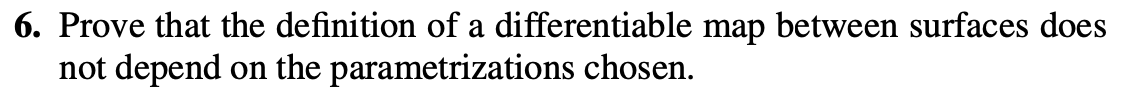
\includegraphics[height=3cm,width=18cm]{HW3a4}
\end{question}
\begin{proof}
Suppose we are given a map $\pi:S_1\rightarrow S_2$ differentiable in the sense of manifold. We know for $\underline{\text{arbitrary}}$ $p$ in  $S_1$, there exists 
\begin{enumerate}[label=(\alph*)]
  \item $\textbf{x}_1:U_1\rightarrow S_1$ (a local parametrization around $p$)
  \item $\textbf{x}_2:U_2\rightarrow S_2$ (a local parametrization around $\pi(p)$)
\end{enumerate}
such that 
\begin{align}
\label{dife}
\Big(\textbf{x}_2^{-1}\circ \pi \circ \textbf{x}_1 \Big):U_1\subseteq \R^2\rightarrow U_2\subseteq \R^2\text{ is a diffeomorphism }
\end{align}
Now, fix two arbitrary 
\begin{enumerate}[label=(\alph*)]
  \item  $\textbf{x}_1':U_1'\rightarrow S_1$ (a local parametrization around $p$)
  \item $\textbf{x}_2':U_2'\rightarrow S_2$ (a local parametrization around $\pi(p)$)
\end{enumerate}
We are required to prove (Note that the domain of each composited function may be smaller, but this does not undermine the validity of our argument, since we only care about the differentiablity at $p$) 
\begin{align*}
\vi{\Big((\textbf{x}_2')^{-1}\circ \pi \circ \textbf{x}_1' \Big):U_1'\subseteq \R^2\rightarrow U_2'\subseteq \R^2\text{ is a diffeomorphism  }}
\end{align*}
Note that 
\begin{align*}
  (\textbf{x}_2')^{-1}\circ \pi \circ \textbf{x}_1' &=(\textbf{x}_2')^{-1}\circ \big( \textbf{x}_2 \circ  \textbf{x}_2^{-1} \big)\circ \pi \circ \big( \textbf{x}_1 \circ \textbf{x}_1^{-1}  \big)\circ  \textbf{x}_1'\\
  &=(\textbf{x}_2')^{-1}\circ \textbf{x}_2 \circ  \textbf{x}_2^{-1} \circ \pi \circ  \textbf{x}_1 \circ \textbf{x}_1^{-1} \circ  \textbf{x}_1'\\\
  &=h_2\circ \textbf{x}_2^{-1} \circ  \pi \circ \textbf{x}_1 \circ h_1
\end{align*}
where
\begin{align*}
\begin{cases}
 h_1\equiv\textbf{x}_1^{-1}\circ \textbf{x}_1':U_1'\rightarrow U_1 \\
 h_2\equiv (\textbf{x}_2')^{-1}\circ \textbf{x}_2:U_2\rightarrow U_2'
\end{cases}\text{ are changes of coordinate }
\end{align*}
Now, because changes of coordinates are diffeomorhphism, and $\textbf{x}_2^{-1}\circ \pi \circ \textbf{x}_1$ is diffeomorphism by \myref{Equation}{dife} (definition), we see that 
\begin{align*}
  (\textbf{x}_2')^{-1}\circ \pi \circ \textbf{x}_1'=h_2\circ \big(\textbf{x}_2^{-1}\circ \pi \circ \textbf{x}_1 \big)\circ h_1\text{ is a diffeomorphism at $(\textbf{x}_1')^{-1}(p)$ }
\end{align*}
This then conclude the proof, since $p$ is arbitrary picked from $S_1$. $\vdone$
\end{proof}
\begin{definition}
\textbf{(Definition of Differentiable function on a regular curve)} Given two regular curve $C_1,C_2$, we say the function $f:C_1\rightarrow C_2$ is differentiable at $p$ if for all local parametrizations  $\textbf{x}_1:I\rightarrow C_1\ni p,\textbf{x}_2:I\rightarrow C_2\ni f(p)$,  we have 
\begin{align*}
\textbf{x}_2^{-1}\circ f\circ \textbf{x}_1\text{ is differentaible as a real to real function }
\end{align*}
\end{definition}
\begin{question}{}{}
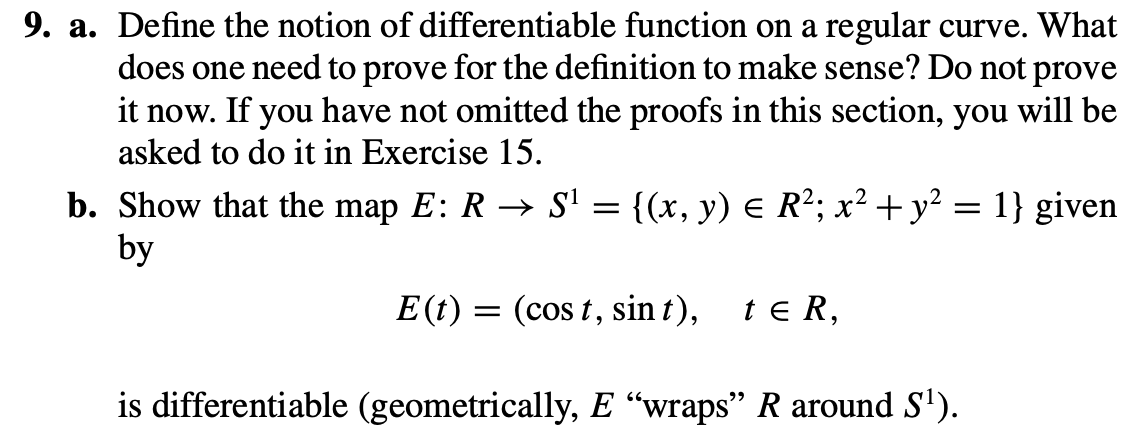
\includegraphics[height=5cm,width=18cm]{HW3a3}
\end{question}
\begin{proof}
Fix $t_0 \inr$. We wish to prove 
\begin{align*}
\vi{E\text{ is differentaible at $t_0$ in the sense of manifold }}
\end{align*}
Locally parametize $t_0$ and $E(t_0)$ by 
\begin{align*}
\textbf{x}_1(t)\triangleq t\text{ and }\textbf{x}_2(t)\triangleq (\cos t,\sin t)
\end{align*}
Now, see that 
\begin{align*}
\textbf{x}_2^{-1}\circ E\circ \textbf{x}_1(t)=t\text{ is clearly differentiable $\vdone$}
\end{align*}
\end{proof}

\begin{question}{}{}
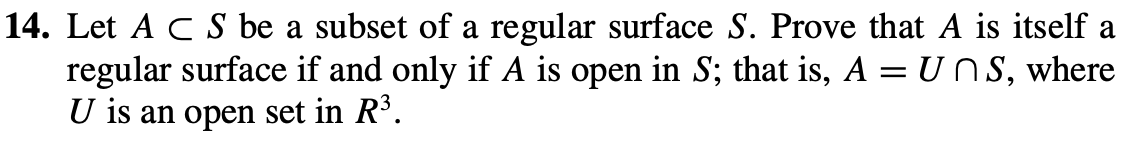
\includegraphics[height=3cm,width=18cm]{HW3a2}
\end{question}
\begin{proof}
$(\longleftarrow)$\\

Fix $a \in A$. Because $a \in S$, we know there exists a local parametrization $\textbf{x}_1:E\rightarrow V\cap S$ around $a$ where $V$ is open in  . Suppose 
\begin{align*}
  E'\triangleq \textbf{x}_1^{-1}[ U\cap V\cap S]
\end{align*}
Now, from 
\begin{enumerate}[label=(\alph*)]
  \item $U\cap V\cap S$ is open in $V\cap S\hspace{1.5cm}(\because U\text{ is open in }\R^3)$ 
  \item $\textbf{x}_1$ is a homeomorphism between $E$ and $V\cap S$ 
  \item $\textbf{x}_1$ is smooth 
  \item $d\textbf{x}_1$ is one-to-one for all $p \in E$
  \item $E'\subseteq E$
\end{enumerate}
We see 
\begin{enumerate}[label=(\alph*)]
  \item $E'$ is open in  $\R^2$
  \item the restriction $\textbf{x}_1|_{E'}$ is a local parametrizaiton around $a$ contained by $A$ 
\end{enumerate}
Because $a$ is arbitrary, this established that $A$ is a regular surface.\\

$(\longrightarrow)$\\

Suppose $A$ is a regular surface. Fix arbitrary $a\in A$. Using Proposition 2.2.3 in Do Carmo, WOLG, we can suppose there exists a chart $\textbf{x}:U\rightarrow \overline{V}\cap S$ around $a$ where $\overline{V}$ is open in $\R^3$ such that 
\begin{align*}
\textbf{x}(x,y)=(x,y,f(x,y))\text{ for some smooth $f$ }
\end{align*}
Because each curve in $A$ lies in  $S$ and  $A$ is itself a regular surface, we see that 
\begin{align*}
T_a(A)=T_a(S)
\end{align*}
This tell us the restriction
\begin{align*}
\textbf{x}|_A\text{ is one-to-one }
\end{align*}
Note that $\textbf{x}$ is smooth. Now by inverse function theorem, it follows that there exists $V$ open in $\R^3$ such that 
 \begin{align*}
\textbf{x}|_{A\cap V}\text{ is a chart around $a$ }
\end{align*}
Now, define $W\triangleq V\cap \overline{V}$. Now, identify 
\begin{align*}
  \textbf{x}|_{A\cap W}\text{ is a chart in both $A$ and  $S$ }
\end{align*}
We now see 
\begin{align*}
A\cap W\text{ is an open neighborhood around $a$ in topology of $S$ }
\end{align*}
This shows that $a \in A^\circ $ in topology of $S$. Because $a$ is arbitrary, it follows that $A$ is open in $S$. 
\end{proof}

\begin{question}{}{}
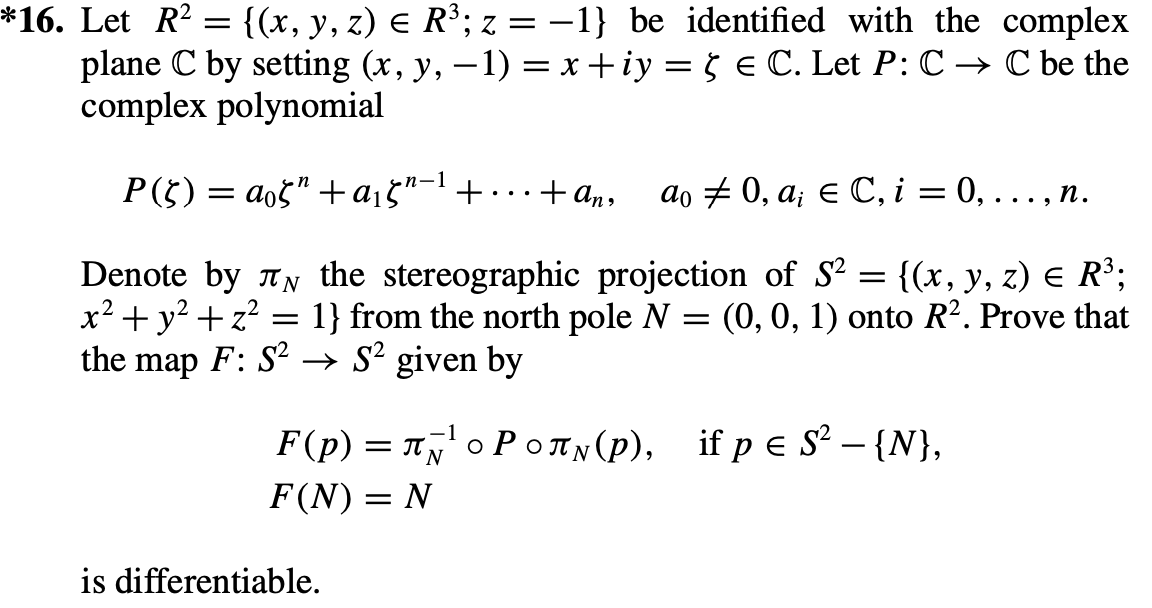
\includegraphics[height=10cm,width=18cm]{HW3a1}
\end{question}
\begin{proof}
Note that 
\begin{align*}
\pi_N(x,y,z)=(\frac{2x}{1-z},\frac{2y}{1-z})\text{ and }\pi_N^{-1}(u,v)=(\frac{4u}{u^2+v^2+4},\frac{4v}{u^2+v^2+4},\frac{u^2+v^2-4}{u^2+v^2+4})
\end{align*}
and that 
\begin{align*}
P(x,y,-1)=\Big(Q(x,y),T(x,y),-1 \Big)\text{ for some $Q,T\inr[x,y]$ }
\end{align*}
It is then now clear that 
\begin{align*}
F\text{ is differentiable on $S^2\setminus N$ }
\end{align*}
Note that 
\begin{align*}
\pi_S(x,y,z)=(\frac{2x}{1+z},\frac{2y}{1+z})\text{ and }\pi_S^{-1}(u,v)=(\frac{4u}{u^2+v^2+4},\frac{4v}{u^2+v^2+4},\frac{-u^2-v^2+4}{u^2+v^2+4})
\end{align*}
Note that 
\begin{align*}
\pi_{S}^{-1}\circ \pi_S\circ F\circ \pi_S^{-1}\circ \pi_S\text{ coincide with $F$ on $S^2\setminus S$}
\end{align*}
Then, we can reduce proving $F$ is differentiable at $N$ into 
\begin{align*}
\vi{\text{ proving }\pi_{S}^{-1}\circ \pi_S\circ F\circ \pi_S^{-1}\circ \pi_S\text{ is differentiable at $N$ }}
\end{align*}
Compute 
\begin{align*}
\pi_N\circ \pi_S^{-1}(u,v)&=\pi_N(\frac{4u}{u^2+v^2+4},\frac{4v}{u^2+v^2+4},\frac{-u^2-v^2+4}{u^2+v^2+4})\\
&=(\frac{4u}{u^2+v^2},\frac{4v}{u^2+v^2})
\end{align*}
Compute
\begin{align*}
\pi_S\circ \pi_N^{-1}(u,v)=(\frac{4u}{u^2+v^2},\frac{4v}{u^2+v^2})
\end{align*}
Note that if we identify $\R^2\setminus 0$ by $\C^*$, we see
\begin{align*}
\hspace{2.5cm}\pi_S\circ \pi_N^{-1}(z)=\pi_N\circ \pi_S^{-1}(z)=\frac{4z}{\abso{z^2}}=\frac{4z}{z\overline{z}}=\frac{4}{\overline{z}}\hspace{1.5cm}(z\inc^*)
\end{align*}
Fix $z\inc^*$. Compute
\begin{align*}
\pi_S\circ F\circ \pi_S^{-1}(z)&=\pi_S \circ \pi_N^{-1}\circ P\circ \pi_N \circ \pi_S^{-1}(z)\\
&=\pi_S\circ \pi_N^{-1}\circ P(\frac{4}{\overline{z}})\\
&=\pi_S \circ \pi_N^{-1}\Big(a_0(\frac{4}{\overline{z}})^n+ \cdots + a_n \Big)\\
&=\frac{4}{\overline{a_0(\frac{4}{\overline{z}})^n+\cdots +a_n}}\\
&=\frac{4}{\overline{a_0}(\frac{4}{z})^n+\cdots +\overline{a_n}}\\
&=\frac{4z^n}{\overline{a_n}z^n+\cdots +\overline{a_0}4^n}
\end{align*}
Compute
\begin{align*}
\pi_S \circ F\circ \pi_S^{-1}(0)=\pi_S \circ F(N)=\pi_S(N)=0
\end{align*}
Then because $a_0\neq 0$. It is now clear that 
\begin{align*}
\hspace{1.5cm}\pi_S\circ F\circ \pi_S^{-1}(z)=\frac{4z^n}{\overline{a_n}z^n+\cdots +\overline{a_0}4^n}\hspace{1.5cm}(z\inc)
\end{align*}
which is differentiable at $0$. Now, we have
\begin{enumerate}[label=(\alph*)]
  \item $\pi_S:S^2\setminus S\rightarrow \C$ is differentiable on $S^2 \setminus S$
  \item $\pi_S\circ F\circ \pi_S^{-1}:\C\rightarrow \C$ is differnetiable on $\C$
   \item $\pi_S^{-1}:\C\rightarrow S^2\setminus S$ is differntiable on $\C$
\end{enumerate}
We can deduce 
\begin{align*}
\pi_S^{-1}\circ \Big(\pi_S\circ F\circ \pi_S^{-1} \Big)\circ \pi_S\text{ is differentiable on $S^2\setminus S\vdone$ }
\end{align*}

Note that we used  \myref{Theorem}{CoDf} in our proof. 
\end{proof}
\begin{theorem}
\label{CoDf}
\textbf{(Composition of Differentiable functions is differentiable)} Given three regular surfaces $\set{S_1,S_2,S_3}$, two differentiable functions $f_1:S_1\rightarrow S_2$ and $f_2:S_2\rightarrow S_3$, we see 
\begin{align*}
f_2\circ f_1\text{ is differentiable on $S_1$ }
\end{align*}
\end{theorem}
\begin{proof}
Fix $p_1\in S_1 $. We wish to prove 
\begin{align*}
  \vi{f_2\circ f_1\text{ is differentiable at $p_1$ }}
\end{align*}
Set 
\begin{enumerate}[label=(\alph*)]
  \item $p_2\triangleq f_1(p_1)$ 
  \item $p_3\triangleq f_2(p_2)$
\end{enumerate}
Let 
\begin{enumerate}[label=(\alph*)]
  \item $\textbf{x}_1:U_1 \rightarrow V_1\cap S_1 \ni p_1 $ be a local parametrzaiton 
   \item $\textbf{x}_2:U_2\rightarrow V_2\cap S_2\ni p_2$ be a local parametrizaiton 
    \item $\textbf{x}_3:U_3\rightarrow V_3\cap S_3\ni p_3$ be a local parametrizaiton 
\end{enumerate}
We wish to prove 
\begin{align*}
  \vi{\textbf{x}_3^{-1}\circ f_2\circ f_1 \circ \textbf{x}_1\text{ is differentiable at $p_1$ }}
\end{align*}
Observe that 
\begin{align*}
\textbf{x}_3^{-1}\circ f_2\circ f_1\circ \textbf{x}_1&=\textbf{x}_3^{-1}\circ f_2 \circ \textbf{x}_2 \circ \textbf{x}_2^{-1} \circ f_1 \circ \textbf{x}_1\\
&=\Big(\textbf{x}_3^{-1}\circ f_2\circ \textbf{x}_2 \Big)\circ \Big(\textbf{x}_2^{-1}\circ f_1\circ \textbf{x}_1 \Big)\text{ is differentiable $\vdone$}
\end{align*}
\end{proof}


\chapter{Surface}
\section{Prerequisite}
\begin{theorem}
\textbf{(Inverse function Theorem)} Given a map $f$ from  $E$ open in $\R^n$ to $\R^n$, if 
\begin{enumerate}[label=(\alph*)]
  \item $f$ is continuously differentiable on $E$ 
  \item $df_a$ is one-to-one 
  \item $a\in E$
\end{enumerate}
Then there exists
\begin{enumerate}[label=(\alph*)]
  \item $U\subseteq E$ open in $E$ where $a\in U$
  \item $V\subseteq \R^n$ open in $\R^n$
\end{enumerate}
Such that 
\begin{align*}
f|_U:U\to V\text{ is a diffeomorphism }
\end{align*}
\end{theorem}
\begin{theorem}
\textbf{(Implicit function Theorem)} Given a map $f$ from an open neighborhood around $(a,b) \in E \subseteq \R^{n+m}\to \R^n$ such that 
\begin{enumerate}[label=(\alph*)]
  \item $f$ is continuously differentiable on $E$
  \item the linear transformation $df_{(a,b)}|_{\R^n}:\R^n \to \R^n$ is one-to-one
  \item $f(a,b)=0$
\end{enumerate}
Then there exists open neighborhood $U$ around $(a,b)\in U \subseteq \R^{n+m}$ and open neighborhood $V$ around  $b  \in V \subseteq \R^m$ such that we can uniquely define a function $g:V \to U$ by 
\begin{align*}
&f(g(y),y)=0\text{ for all $y \in V$}\\
&\text{ and }g\text{ is continuously differentiable with }dg_b=- (df_{(a,b)}|_{\R^n})^{-1}\circ df_{(a,b)}|_{\R^m}
\end{align*}
\end{theorem}
\section{Equivalent Definition of Regular Surface}
\begin{definition}
\textbf{(Definition of Regular Surface: Local Parametrization)} We say a set $S\subseteq \R^3$ is a regular surface if for all $p \in S$ there exists 
\begin{enumerate}[label=(\alph*)]
  \item an open neighborhood $p \in V\subseteq \R^3$
  \item an open set $U\subseteq \R^2$
  \item a function $\textbf{x}:U\rightarrow V\cap S$
\end{enumerate}
such that $\textbf{x}$ satisfy
\begin{enumerate}[label=(\alph*)]
  \item $\textbf{x}$ is smooth 
  \item $\textbf{x}$ is a homemomorphism between $U$ and  $V\cap S$
  \item $d\textbf{x}_q \in L(\R^2,\R^3)$ is one-to-one for all $q\in U$ 
\end{enumerate}
\end{definition}
\begin{definition}
\textbf{(Definition of Regular Surface: Implicit function)} We say a set $S\subseteq \R^3$ is a regular surface if for all $p \in S$ there exists 
\begin{enumerate}[label=(\alph*)]
  \item an open neighborhood $p \in V\subseteq \R^3$ 
  \item a function $F:V\rightarrow \R$ 
\end{enumerate}
such that $F$ satisfy
\begin{enumerate}[label=(\alph*)]
  \item $dF_q$ is onto for all $q\in V\cap S$
  \item $F$ is smooth on  $V$
  \item $\exists c_0\inr, V\cap S=\bset{(x,y,z)\in V:F(x,y,z)=c_0}$
\end{enumerate}
\end{definition}
\begin{mdframed}
We now verify the equivalency between the two definitions. 
\end{mdframed}
\begin{theorem}
\textbf{(Implicit function definition $\longrightarrow$ Local parametrization definition)} 
\end{theorem}
\begin{proof}
Fix $p \in S$. We are given an open neighborhood $p \in V \subseteq \R^3$ and a function $F:V\rightarrow \R$ such that, WOLG, 
\begin{enumerate}[label=(\alph*)]
  \item $dF_q$ is onto for all $q\in V\cap S$
  \item $F$ is smooth on  $V$
  \item $V\cap S=\bset{(x,y,z)\in V: F(x,y,z)=0}$ 
\end{enumerate}


We wish to find 
\begin{align*}
\vi{\text{ a local parametrization $\textbf{x}$ around $p$ }}
\end{align*}
Define $f:V \rightarrow \R^3$ by 
\begin{align*}
f(x,y,z)=(x,y,F(x,y,z))
\end{align*}
Because $dF_p\neq 0$, WOLG, we can suppose $\partial _zF(p)\neq 0$. Now, see 
\begin{align*}
\text{det}(df)=\begin{vmatrix}
  1 & 0 & 0\\
  0 & 1 & 0\\
  \partial_x F & \partial_y F & \partial _z F
\end{vmatrix}\neq 0
\end{align*}
Now, note that 
\begin{enumerate}[label=(\alph*)]
  \item $f$ is smooth on $V\hspace{0.5cm}(\because \text{ $F$ is smooth on $V$ })$  
  \item $df_p$ is one-to-one $\hspace{0.5cm}(\because \partial_zF(p)\neq 0)$  
\end{enumerate}
Then, by inverse function Theorem, we know  
\begin{align*}
f\big|_{V'}\to U'\text{ is a local diffeomorphism around $V'\ni p$ and around $U'\ni f(p)$}
\end{align*}
Let $U\subseteq \set{(x,y,0):(x,y)\inr^2}$ be an open-neighborhood around $f(p)$ contained by $U'$. We claim  
\begin{align*}
  \vi{\textbf{x}\triangleq f^{-1}\big|_U\text{ suffices }}
\end{align*}
Note that $\textbf{x}$ is well-defined since $U\subseteq U'$ and $f$ is a bijective between  $V'$ and $U'$.\\


Also, note that $\textbf{x}$ do maps points in $U$ to points in $V\cap S$, since $V\cap S=\bset{(x,y,z)\in V:F(x,y,z)=0}$.\\

Suppose that 
\begin{align*}
\begin{bmatrix}
  \alpha_{1,1} & \alpha_{1,2} & \alpha _{1,3}\\
  \alpha _{2,1} & \alpha _{2,2} & \alpha _{2,3}\\
  \alpha _{3,1} & \alpha _{3,2} & \alpha _{3,3}
\end{bmatrix}\triangleq df^{-1}_\alpha  =\big(df_{f^{-1}(\alpha )} \big)^{-1}\text{ for all $\alpha \in U$ }
\end{align*}
We clearly have 
\begin{align*}
d\textbf{x}=\begin{bmatrix}
  \alpha_{1,1} & \alpha _{1,2}\\
  \alpha _{2,1} & \alpha _{2,2}\\
  \alpha_{3,1} & \alpha_{3,2}
\end{bmatrix}
\end{align*}
Now, one can use the premise 
\begin{align*}
dF_q\text{ is onto for all } q\in V\cap S
\end{align*}
to check $\textbf{x}$ do satisfy the regular condition. (Compute $\text{det}(df_{\alpha }^{-1})$ using co-factor formula on the third column) $\vdone$
\end{proof}
\begin{mdframed}

\end{mdframed}
\begin{definition}
\textbf{(Definition of Regular surface: Monge Patches)} We say a set $S\subseteq \R^3$ is a regular surface if for all $p \in S$ there exists some open neighborhood $ p \in V\subseteq \R^3$ such that 
\begin{center}
   \begin{minipage}{0.9\linewidth}  

$V\cap S$   can be expressed as the graph of some smooth function $f:O\subseteq \R^2 \rightarrow \R$ in the sense that one of the followings hold 
   \end{minipage}
\end{center}
\begin{enumerate}[label=(\alph*)]
  \item $V\cap S=\set{(x,y,f):(x,y)\in O}$ for some smooth $f:O \subseteq \R^2 \rightarrow \R$
  \item $V\cap S=\set{(x,f,z):(x,z)\in O}$ for some smooth $f:O \subseteq \R^2 \rightarrow \R$
  \item $V\cap S=\set{(f,y,z):(y,z)\in O}$ for some smooth $f:O \subseteq \R^2 \rightarrow \R$
\end{enumerate}
\end{definition}
\section{Differentiable Mapping Between Regular Surfaces}
\begin{theorem}
\label{CoP}
\textbf{(Change of Parameter is a diffeomorphism)} Let $p$ be a point of a regular surface $S$, and let $\textbf{x}_1:U_1\rightarrow S$ and $\textbf{x}_2:U_2\rightarrow S$ be two charts containing $p$. Define $W\triangleq \textbf{x}_1(U_1)\cap \textbf{x}_2(U_2)\cap S$. Then 
\begin{align*}
  \text{ The \textbf{change of coordinate } $h\triangleq \textbf{x}_2^{-1}\circ \textbf{x}_1:\textbf{x}_1^{-1}(W)\to \textbf{x}_2^{-1}(W)$ is a diffoeomorphism }
\end{align*}
\end{theorem}
\begin{proof}
Note the symmetry of $h$ and $h^{-1}$. WOLG, we only have to prove 
\begin{align*}
\vi{h:\textbf{x}_1^{-1}(W)\rightarrow \textbf{x}_2^{-1}(W)\text{ is differentiable }}
\end{align*}
Fix $r \in \textbf{x}_1^{-1}(W)$. We prove 
\begin{align*}
  \vi{h\text{ is differentiable at $r$ }}
\end{align*}
Define $q\triangleq h(r)$. Express $\textbf{x}_2$ by 
\begin{align*}
\textbf{x}_2(u,v)=(x,y,z)
\end{align*}
Because $(d\textbf{x}_2)_q$ is one-to-one, WOLG, we have 
\begin{align*}
\begin{vmatrix} 
  \partial_u x & \partial_v x\\
  \partial_u y & \partial_v y
\end{vmatrix}(q)\neq 0
\end{align*}
Now, define $F:\textbf{x}_2^{-1}(W)\times \R\rightarrow \R^3$ by  
\begin{align}
\label{CC1}
F(u,v,t)\triangleq  \Big(x(u,v),y(u,v),z(u,v)+t \Big)
\end{align}
Compute 
\begin{align*}
  \text{det}(dF_{(q,0)})=\begin{vmatrix}
  \partial_u x & \partial_v x & 0\\
  \partial_u y & \partial_v y & 0\\
  \partial_u z & \partial_v z & 1 
\end{vmatrix}(q,0)\neq 0 
\end{align*}
Then by Inverse function Theorem, we see that there exists an open neighborhood $M\subseteq \R^3$ around $F(q,0)$ such that $F^{-1}$ exists and is differentiable on $M$.\\

Now, from \myref{Equation}{CC1}, note that 
\begin{align*}
F(u,v,0)=\textbf{x}_2(u,v)
\end{align*}
Recall the definition $h$, we now have 
\begin{align*}
h=\textbf{x}_2^{-1}\circ \textbf{x}_1=F^{-1}\circ \textbf{x}_1\text{ on $\textbf{x}_1^{-1}(M)$ }
\end{align*}
Then because 
\begin{enumerate}[label=(\alph*)]
  \item $\textbf{x}_1$ is differentiable at $r$ 
   \item $F^{-1}$ is differentiable at $F(q,0)=\textbf{x}_2(q)=\textbf{x}_1(r)$ 
\end{enumerate}
We see $h$ is indeed differentiable at $r\vdone$
\end{proof}
\begin{mdframed}
Now, given two regular surfaces $S_1,S_2$, a set  $E\subseteq S_1$ open in $S_1$, and a function  $f:E\rightarrow S_2$, we can say $f$ is \textbf{differentiable at $p\in  E$} if there exists some local charts $\textbf{x}_1:U_1 \rightarrow S_1,\textbf{x}_2:U_2\rightarrow S_2$, containing $p,f(p)$ such that 
\begin{enumerate}[label=(\alph*)]
  \item there exists $\epsilon $ small enough such that $B_{\epsilon }(\textbf{x}_1^{-1}(p))\subseteq U_1$ and $\textbf{x}_2^{-1}\circ f\circ \textbf{x}_1$ is defined on $B_\epsilon (\textbf{x}_1^{-1}(p))$ 
  \item $\textbf{x}_2^{-1}\circ f\circ \textbf{x}_1:B_\epsilon (\textbf{x}_1^{-1}(p))\rightarrow U_2$ is differentiable at $\textbf{x}_1^{-1}(p)$
\end{enumerate}
One can check that if $f:E\rightarrow S_2$ is differetnaible at $p$, then  $f:E\rightarrow S_2$ must be continuous at  $p$. Also, using \myref{Theorem}{CoP}, one can check that if $f$ is differnetiable at $p$, then every local charts  $\textbf{x}_3:U_3\rightarrow S_1,\textbf{x}_4:U_4\rightarrow S_2$ containing $p,f(p)$ satisfy 
\begin{align*}
\textbf{x}_4^{-1}\circ f\circ \textbf{x}_3\text{ is differentiable at $\textbf{x}_3^{-1}(p)$ }
\end{align*}
Thus, if we wish to check whether some function $f:E\rightarrow S_2$ is differentiable at $p$, every pair of local charts respectively containing  $p,f(p)$ can be used.
\end{mdframed}
\begin{theorem}
\label{CoD}
\textbf{(Composition of Differentiable functions is differentiable)} Given three regular surfaces $S_1,S_2,S_3$, two differentiable functions $f_1:S_1\rightarrow S_2$ and $f_2:S_2\rightarrow S_3$, we see 
\begin{align*}
f_2\circ f_1\text{ is differentiable on $S_1$ }
\end{align*}
\end{theorem}
\begin{proof}
Fix $p_1\in S_1 $. We wish to prove 
\begin{align*}
  \vi{f_2\circ f_1\text{ is differentiable at $p_1$ }}
\end{align*}
Set 
\begin{align*}
p_2\triangleq f_1(p_1)\text{ and }p_3\triangleq f_2(p_2)
\end{align*}
Let 
\begin{enumerate}[label=(\alph*)]
  \item $\textbf{x}_1:U_1 \rightarrow S_1 \ni p_1 $ be a local chart 
   \item $\textbf{x}_2:U_2\rightarrow S_2\ni p_2$ be a local chart
    \item $\textbf{x}_3:U_3\rightarrow  S_3\ni p_3$ be a local chart
\end{enumerate}
We wish to prove 
\begin{align*}
  \vi{\textbf{x}_3^{-1}\circ f_2\circ f_1 \circ \textbf{x}_1\text{ is differentiable at $p_1$ }}
\end{align*}
Observe that 
\begin{align*}
\textbf{x}_3^{-1}\circ f_2\circ f_1\circ \textbf{x}_1&=\textbf{x}_3^{-1}\circ f_2 \circ \textbf{x}_2 \circ \textbf{x}_2^{-1} \circ f_1 \circ \textbf{x}_1\\
&=\Big(\textbf{x}_3^{-1}\circ f_2\circ \textbf{x}_2 \Big)\circ \Big(\textbf{x}_2^{-1}\circ f_1\circ \textbf{x}_1 \Big)\text{ is differentiable $\vdone$}
\end{align*}
\end{proof}

\section{Equivalent Definition of Tangent Plane}

\begin{definition}
\textbf{(Definition of Tangent Plane: Space of Tangent Vectors)} Given a regular surface $S$ and $p\in  S$, we define \textbf{tangent plane $T_pS$ to $S$ at $p$} by 
\begin{align*}
T_pS=\set{\alpha '(0)\inr^3|\hspace{0.1cm}\alpha:I\rightarrow S \text{ is a smooth curve  passing through $p$ at $\alpha (0)$ }}
\end{align*}
\end{definition}
\begin{definition}
\textbf{(Definition of Tangent Plane: Local Parametrization)} Given a regular surface $S$, that $p\in  S$ and a local parametrzaiton $\textbf{x}:(u,v)\mapsto  (x,y,z)$ around $p$ such that $\textbf{x}(q)=p$,  we define \textbf{tangent plane $T_pS$ to  $S$ at $p$} by 
\begin{align*}
T_pS=d\textbf{x}(\R^2)
\end{align*}
\end{definition}
\begin{theorem}
\textbf{(Equivalence of Definitions)} Given a regular surface $S$, $p\in  S $ and a local chart $\textbf{x}:U\rightarrow S$ containing $p$ such that $\textbf{x}(q)=p$, we have 
\begin{align*}
d\textbf{x}_q(\R^2)=\set{\alpha '(0)\inr^3|\alpha:(-\epsilon ,\epsilon )\rightarrow S\text{ satisfy }\alpha (0)=p}
\end{align*}
\end{theorem}
\begin{proof}
We first prove 
\begin{align*}
\vi{d\textbf{x}_q(\R^2)\subseteq \set{\alpha '(0)\inr^3|\alpha:(-\epsilon ,\epsilon )\rightarrow S\text{ satisfy }\alpha (0)=p}}
\end{align*}
Fix $w\in d\textbf{x}_q(\R^2)$. We reduce the problem into 
\begin{align*}
\vi{\text{ constructing smooth $\alpha :(-\epsilon ,\epsilon )\rightarrow S$ such that $\alpha (0)=p$ and $\alpha '(0)=w$ }}
\end{align*}
We know there exists $v \inr^2$ such that $d\textbf{x}_q(v)=w$. Define $\gamma :(-\epsilon ,\epsilon )\rightarrow U$ by 
\begin{align*}
\gamma (t)= tv+q
\end{align*}
We claim 
\begin{align*}
  \vi{\alpha =\textbf{x}\circ \gamma :(-\epsilon ,\epsilon )\rightarrow S\text{ suffices }}
\end{align*}
Note that $\textbf{x}\circ \gamma (0)=\textbf{x}(q)=p$ and
\begin{align*}
(\textbf{x}\circ \gamma )'(0)=d\textbf{x}_q(\gamma '(0))=d\textbf{x}_q(v)=w \vdone 
\end{align*}
We now prove 
\begin{align*}
\blue{\set{\alpha '(0)\inr^3|\alpha:(-\epsilon ,\epsilon )\rightarrow S\text{ satisfy }\alpha (0)=p}\subseteq d\textbf{x}_q(\R^2)}
\end{align*}

Fix a smooth curve $\alpha :(-\epsilon ,\epsilon ) \rightarrow S$ passing through $p$ at $\alpha (0)$. We wish 
\begin{align*}
\blue{\text{ to show }\alpha '(0)\in d\textbf{x}_q(\R^2)}
\end{align*}
Define $\beta :(-\epsilon ,\epsilon )\rightarrow U$ by 
\begin{align*}
\beta (t)=\textbf{x}^{-1}\circ \alpha (t)
\end{align*}
We claim 
\begin{align*}
\blue{\alpha '(0)=d\textbf{x}_q(\beta '(0))}
\end{align*}
Compute using Chain Rule 
\begin{align*}
\beta '(0)=(d\textbf{x}^{-1})_p\circ \alpha '(0)
\end{align*}
Note that $(d\textbf{x}^{-1})_p=(d\textbf{x}_q)^{-1}$. This then give us 
\begin{align*}
  d\textbf{x}_q(\beta '(0))=d\textbf{x}_q \circ (d\textbf{x}^{-1})_p \circ \alpha '(0)=\alpha '(0)\bdone
\end{align*}
\end{proof}
\begin{mdframed}
Now, given a differentiable function $f$ between two regular surface $S_1,S_2$, we can define the \textbf{derivative} $df$ of $f$ 
\end{mdframed}
\begin{definition}
\textbf{(Derivative of Differntiable mapping between regular surface)} Given a differentiable mapping $f:S_1\rightarrow S_2$, we define $df_p:T_pS_1\to T_{f(p)}S_2$ by 
\begin{align*}
df_p(\alpha '(0))\triangleq (f\circ \alpha )'(0)
\end{align*}
\end{definition}
\begin{theorem}
\textbf{(Derivative is well-defined and linear)}
\end{theorem}
\begin{proof}
Fix local charts $\textbf{x}(u,v)$ containing $p$ and $\overline{\textbf{x}}(\overline{u},\overline{v})$ containing $f(p)$. Express $f$ locally in coordinate 
\begin{align*}
f(u,v)=(f_1(u,v),f_2(u,v))
\end{align*}
Express $\alpha(t)$ in the form 
\begin{align*}
\alpha (t)=(u(t),v(t))
\end{align*}
We now have 
\begin{align*}
  (f\circ \alpha )(t)=(f_1(u,v),f_2(u,v))(t)
\end{align*}
Compute 
\begin{align}
\label{falpha}
  (f\circ \alpha )'(0)&=\Big(\big(\frac{\partial f_1}{\partial u},\frac{\partial f_1}{\partial v} \big)(p)\cdot \alpha '(0),\big(\frac{\partial f_2}{\partial u},\frac{\partial f_2}{\partial v} \big)(p)\cdot \alpha '(0)  \Big)
\end{align}
This shows that $(f\circ \alpha )'(0)$ is only determined by $\alpha '(0)$ and $f$. Thus, our definition is well defined, and from (\myref{}{falpha}), it is easily checked that $df_p$ is linear.  
\end{proof}
\section{First Fundamental Form}
\begin{definition}
\textbf{(First Fundamental Form)} Given a regular surface $S$ and $p\in  S$, by \textbf{the first fundamental form of $S$ at $p$}, we mean a function $I_p:T_p(S)\rightarrow \R$ defined by 
\begin{align*}
I_p(w)\triangleq w\cdot w
\end{align*}
\end{definition}
\begin{mdframed}
Given a local chart $\textbf{x}(u,v):U\rightarrow S$, we can define three real valued- function $E,F,G: U\rightarrow \R$ by 
\begin{align*}
E(u,v)&\triangleq  \abso{\partial_u \textbf{x}(u,v)}^2 \\
F(u,v)&\triangleq  \partial_u\textbf{x}(u,v)\cdot \partial_v \textbf{x}(u,v)\\
G(u,v)&\triangleq \abso{\partial_v \textbf{x}(u,v)}^2
\end{align*}
These three functions help us compute the arc-length of a smooth curve that lies in $\textbf{x}(U)$. Suppose $\alpha (t)$ lies in $\textbf{x}(U)$, and express 
\begin{align*}
\alpha (t)=\textbf{x}(u(t),v(t))
\end{align*}
Note that the expression give us 
\begin{align*}
\alpha'(t)=d\textbf{x}(u'(t),v'(t))=u'(t)\partial_u \textbf{x}(u(t),v(t))+v'(t)\partial_v \textbf{x}(u(t),v(t))\text{ where $q=\alpha (t)$ }
\end{align*}
We see that 
\begin{align*}
  \int_0^r \abso{\alpha '(t)}dt&= \int_0^r \sqrt{\alpha '(t)\cdot \alpha '(t)} dt\\
  &=\int_0^r \sqrt{\big(u'(t)\partial_u \textbf{x}(q)+v'(t)\partial_v \textbf{x}(q) \big)\cdot \big(u'(t)\partial_u \textbf{x}(q)+v'(t)\partial_v \textbf{x}(q) \big)}dt\\
  &=\int_0^r \sqrt{E(q)\big(u'(t) \big)^2 + 2F(q)u'(t)v'(t)+G(q)\big(v'(t) \big)^2} dt
\end{align*}
These three functions also help us define and compute the area of some bounded region $Q$ that lies in $\textbf{x}(U)$. Suppose we define the area of $Q$ by 
\begin{align*}
A(Q)=\iint_Q \abso{\textbf{x}_u \times \textbf{x}_v} dudv 
\end{align*}
One can rigorously by computation in component to justify the following  
\begin{align*}
\abso{v\times w}^2 + (v\cdot w)^2= (\sin^2 \theta+ \cos^2 \theta)\abso{v}^2\abso{w}^2= \abso{v}^2\abso{w}^2
\end{align*}
This then give us 
\begin{align*}
  \iint_Q \abso{\textbf{x}_u \times \textbf{x}_v}dudv &= \iint_Q \sqrt{ \abso{\textbf{x}_u}^2\abso{\textbf{x}_v}^2-(\textbf{x}_u \cdot \textbf{x}_v)^2}  dudv\\
&=\iint_Q \sqrt{EG-F^2}dudv 
\end{align*}
Also, note that the angle of two coordinates can also be computed by 
\begin{align*}
\cos \theta = \frac{\textbf{x}_u \cdot \textbf{x}_v }{\abso{\textbf{x}_u}\abso{\textbf{x}_v}}=\frac{F}{\sqrt{EG} }
\end{align*}

\end{mdframed}
\begin{mdframed}
!!!!! Show that given a stereographical projection $\textbf{x}:\R^2 \times 0 \rightarrow S^2\setminus N$ preserve angle. Prove that given $v,w \inr^2$ starting at $p\inr^2$, we have 
\begin{align*}
\frac{d\textbf{x}_q(v)\cdot d\textbf{x}_q(w)}{\abso{d\textbf{x}_q(v)}\abso{d\textbf{x}_q(w)}}=v\cdot w
\end{align*}
So, we can show that  $\textbf{x}:\R^2 \rightarrow S^2 \setminus N$ satisfy 
\begin{align*}
d\textbf{x}(v)\cdot d\textbf{x}(w)= C (v\cdot w)\text{ where }C\text{ is a constant }
\end{align*}
is conformal (preserving angle). 
\end{mdframed}
\section{HW4}
\begin{question}{}{}
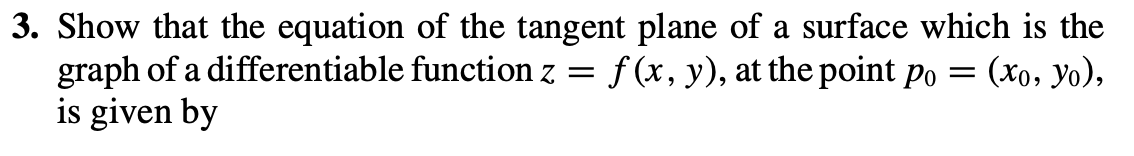
\includegraphics[height=3cm,width=18cm]{hw4q1}
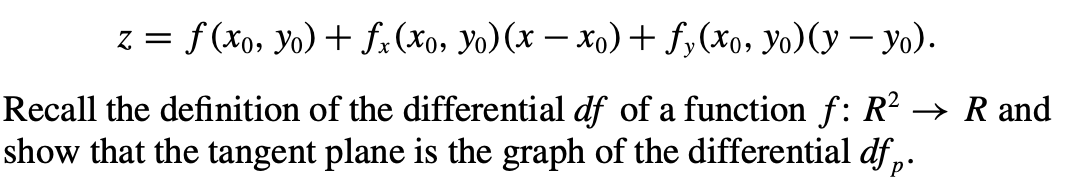
\includegraphics[height=3cm,width=18cm]{hw4q1a}
\end{question}
\begin{proof}
The question first ask us to prove 
\begin{align*}
\vi{T_{p_0}(S)=\set{(x,y,z)\inr^3: z=f(x_0,y_0)+(x-x_0)\partial_x f(p_0)+(y-y_0)\partial_y f(p_0)}}
\end{align*}
By premise of the question, we know there exists a global chart $\textbf{x}$  
 \begin{align*}
\textbf{x}(x,y)\triangleq (x,y,f(x,y))
\end{align*}
Compute 
\begin{align*}
d\textbf{x}=\begin{bmatrix}
  1 & 0 \\
  0 & 1\\
  \partial_x f & \partial_y f
\end{bmatrix}
\end{align*}
This tell us 
\begin{align*}
T_{p_0}(S)&=(x_0,y_0,f(x_0,y_0))+\text{span}(\begin{bmatrix}
  1 \\
  0\\
  \partial_x f(p_0)
\end{bmatrix},\begin{bmatrix}
0\\
1\\
\partial_y f(p_0)
\end{bmatrix})\\
&=\set{(x,y,z)\inr^3: z=f(x_0,y_0)+(x-x_0) \partial_x f(p_0)+(y_y_0) \partial_y f(p_0)}\vdone
\end{align*}
Compute 
\begin{align*}
df_{p_0}=\begin{bmatrix}
  \partial_x f(p_0) & \partial_y f(p_0)
\end{bmatrix}
\end{align*}
Then we see 
\begin{align*}
T_{p_0}(S)=(x_0,y_0,f(x_0,y_0))+ \set{(x,y,df_{p_0}(x,y))\inr^3: (x,y)\inr^2}
\end{align*}
where the right hand side is the graph of $df_{p_0}$ when the origin is set to be $(p_0,f(p_0))$ 







\end{proof}
\begin{question}{}{}
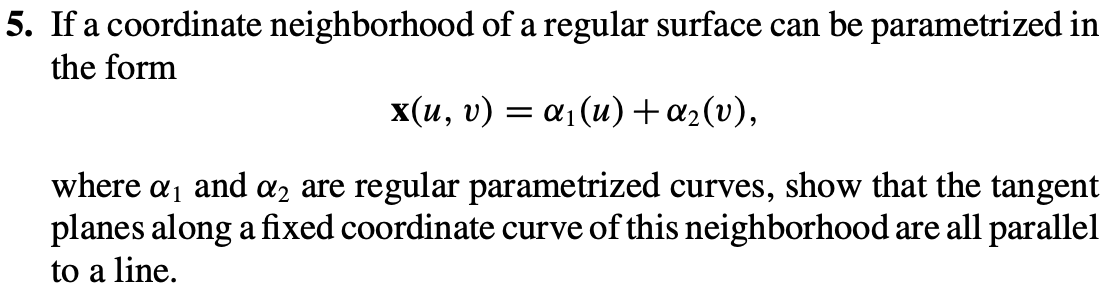
\includegraphics[height=7cm,width=18cm]{hw4q2}
\end{question}
\begin{proof}
WOLG, suppose the coordinate curve $\gamma :I\rightarrow S$ is  
\begin{align*}
\gamma  (t)=\textbf{x}(u_0,t)
\end{align*}
Compute 
\begin{align*}
d\textbf{x}=\begin{bmatrix}
  \alpha_1' (u) & \alpha _2'(v)
\end{bmatrix}\text{ and }d\textbf{x}_{\gamma (t)}=\begin{bmatrix}
  \alpha_1'(u_0)& \alpha_2'(v)
\end{bmatrix}
\end{align*}
Then see that 
\begin{align*}
T_{\gamma (t)} (S)=\text{span}(\alpha_1'(u_0),\alpha_2'(t))
\end{align*}
Since $\alpha_1'(u_0)$ is fixed, we see $T_{\gamma (t) }(S)$ are all parallel to $\alpha_1'(u_0)$. 
\end{proof}
\begin{question}{}{}
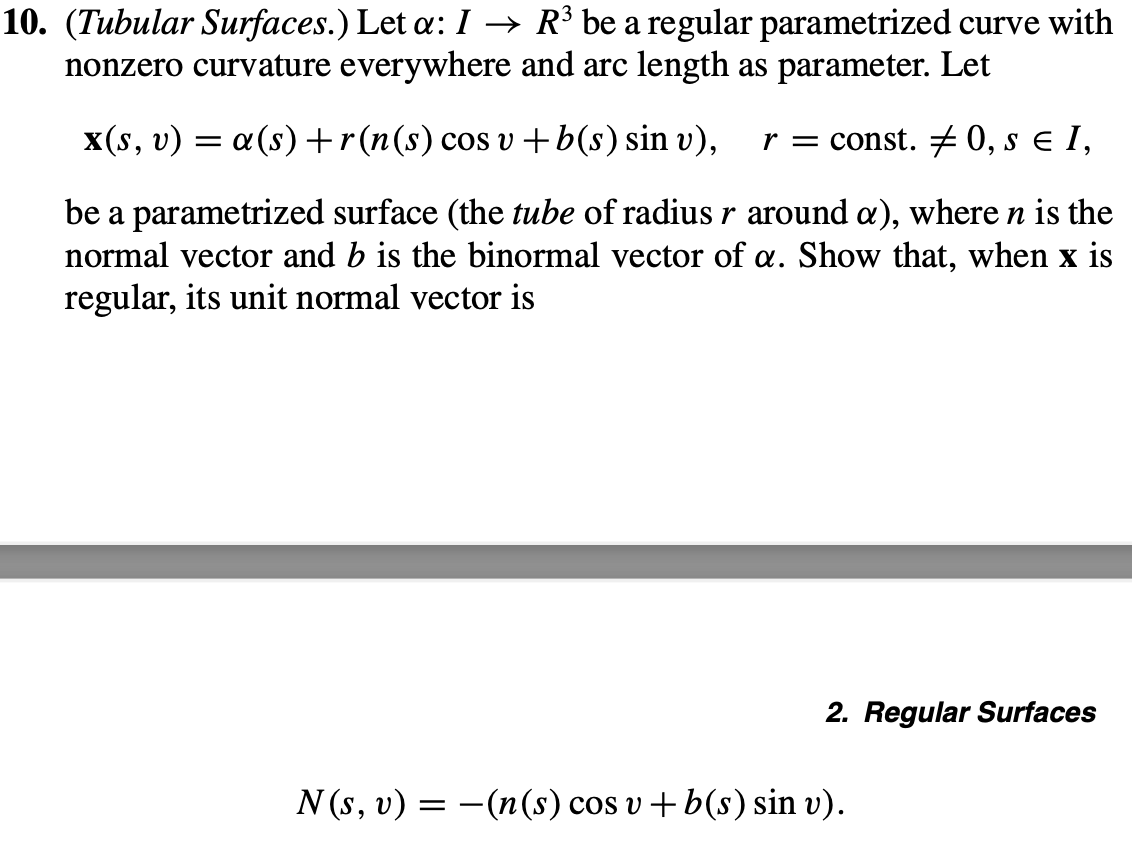
\includegraphics[height=13cm,width=18cm]{hw4q3}
\end{question}
\begin{proof}
Use Frenet-Serret Formula to compute 
\begin{align*}
d\textbf{x}= \begin{bmatrix}
  \alpha '+r \big((-\kappa T-\tau B)\cos v+ \tau N \sin v \big) & r(-N \sin v+ B \cos v)
\end{bmatrix}
\end{align*}
We wish to show 
\begin{align*}
  \vi{-(N \cos v+B \sin v)\perp d\textbf{x}(\R^2)}
\end{align*}
We then only have to prove 
\begin{align*}
&\vi{\big(N \cos v+B \sin v \big)\perp -N \sin v + B \cos v} \\
  \text{ and }&\vi{\big(N \cos v+B \sin v \big) \perp \alpha' + r  \big((-\kappa T-\tau B)\cos v+ \tau N \sin v \big)}
\end{align*}
Because $\set{T,N,B}$ form an othothonormal basis and $\alpha '$ is just $T$, we have 
\begin{align*}
  (N \cos v + B \sin v)\cdot (-N \sin v+ B \cos v)=-(\cos v \sin v)+\sin v \cos v=0
\end{align*}
and have 
\begin{align*}
  &(N \cos v + B \sin v)\cdot \Big(\alpha '+r\big((-\kappa T-\tau B)\cos v + \tau N \sin v \big) \Big)\\
  &= r\tau \cos v \sin v- r \tau \sin v \cos v=0 \vdone
\end{align*}
\end{proof}
\begin{question}{}{}
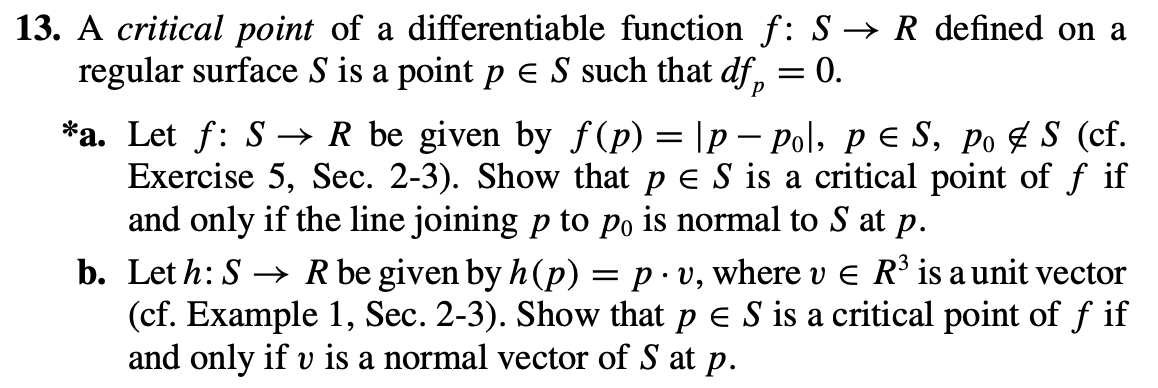
\includegraphics[height=10cm,width=18cm]{hw4q4}
\end{question}
\begin{proof}
Compute 
\begin{align*}
dh_p(\alpha '(0))=\frac{d}{dt}h(\alpha (t))|_{t=0}=v\cdot \alpha '(0)
\end{align*}
In other words, 
\begin{align*}
dh_p(w)=v\cdot w
\end{align*}
This implies 
\begin{align*}
dh_p(l)=0,\forall l\in T_p(S)\iff v\perp T_p(S)\iff  v\text{ is a normal vector of $S$ at $p$ }
\end{align*}
\end{proof}





\begin{question}{}{}
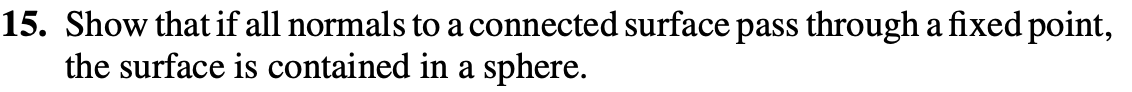
\includegraphics[height=3cm,width=18cm]{hw4q5}
\end{question}
\begin{proof}
WOLG, suppose the fixed point is the origin. Let $S$ be the regular surface. We are given the fact that any local chart $\textbf{x}(u,v)$ satisfy the equation 
\begin{align}
\label{lca}
\textbf{x}(u,v)=f_{\textbf{x}}(u,v)N(u,v)
\end{align}
where $f_\textbf{x}(u,v)$ is a scalar-valued function and $N(u,v)$ is the unit normal vector of $S$ at $\textbf{x}(u,v)$. We first show that 
\begin{align*}
\vi{\text{ the distance of the surface to the origin is locally a constant }}
\end{align*}
In other words, we wish to prove that any local chart $\textbf{x}(u,v)$ satisfy 
\begin{align*}
  \vi{f_\textbf{x}\text{ is constant on domain of $\textbf{x}$ }}
\end{align*}
Doing partial derivative on $N\cdot N=1$, we see that 
\begin{align*}
\partial_u N\perp N \text{ and }\partial_v N\perp N
\end{align*}
This implies 
\begin{align*}
\partial_u N, \partial _v N \in T_p(S)
\end{align*}
We know 
\begin{align*}
\partial_u \textbf{x},\partial_v \textbf{x}\in T_p(S)
\end{align*}
Now, doing partial derivative on both side of (\myref{}{lca}), we see
\begin{align*}
\partial_u \textbf{x}=(\partial_u f_\textbf{x})N+f_\textbf{x}(\partial_u N)\text{ and }\partial_v \textbf{x}=(\partial_v f_\textbf{x})N+ f_\textbf{x} (\partial_v N)
\end{align*}
and see 
\begin{align*}
  (\partial_uf_\textbf{x})N=\partial_u \textbf{x}-f_\textbf{x}(\partial_u N)\in T_p(S)\text{ and }  (\partial_vf_\textbf{x})N=\partial_v \textbf{x}-f_\textbf{x}(\partial_v N)\in T_p(S)
\end{align*}
Then because $N\not\in T_p(S)$, we can conclude $\partial_uf_\textbf{x}=\partial_v f_\textbf{x}=0$. This establish that $f_\textbf{x}$ is a constant.  $\vdone$\\

Note that the surface is connected, this implies that the distance of the surface to the origin is globally a constant, which implies the surface is contained in a sphere.

\end{proof}
\begin{question}{}{}
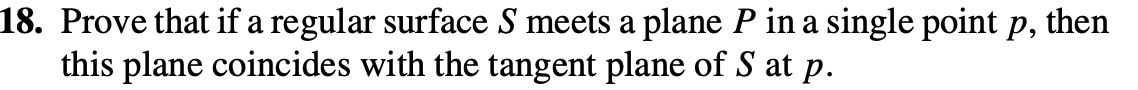
\includegraphics[height=3cm,width=18cm]{hw4q6}
\end{question}
\begin{proof}
WOLG, suppose $P$ is the  $x,y$-plane, $p$ is the origin and $S\subseteq \set{(x,y,z)\inr^3: z\geq 0}$ (This can be achieved by a rigid motion). We wish to show 
\begin{align*}
  \vi{T_p(S)=P}
\end{align*}
Because  $\text{dim}(T_pS)=\text{dim}(P)=2$, we can reduce the problem into proving 
\begin{align*}
  \vi{T_p(S)\subseteq P}
\end{align*}
Fix $w \in T_p(S)$. We reduce the problem into 
\begin{align*}
\vi{\text{ proving }w\in P}
\end{align*} 
Let $\alpha:(-\epsilon ,\epsilon )\rightarrow S$ satisfy 
\begin{align*}
\alpha (0)=0\text{ and }\alpha '(0)=w
\end{align*}
Express 
\begin{align*}
\alpha (t)\triangleq (x,y,z)
\end{align*}
Because $S$ is above $P$, the $x,y$-plane, we know  $z$ attain minimum at $0$. This implies $z'(0)=0$, and implies $\alpha '(0)=(x'(t),y'(0),0)\in P$ (the $x,y$-plane) $\vdone$
\end{proof}
\begin{question}{}{}
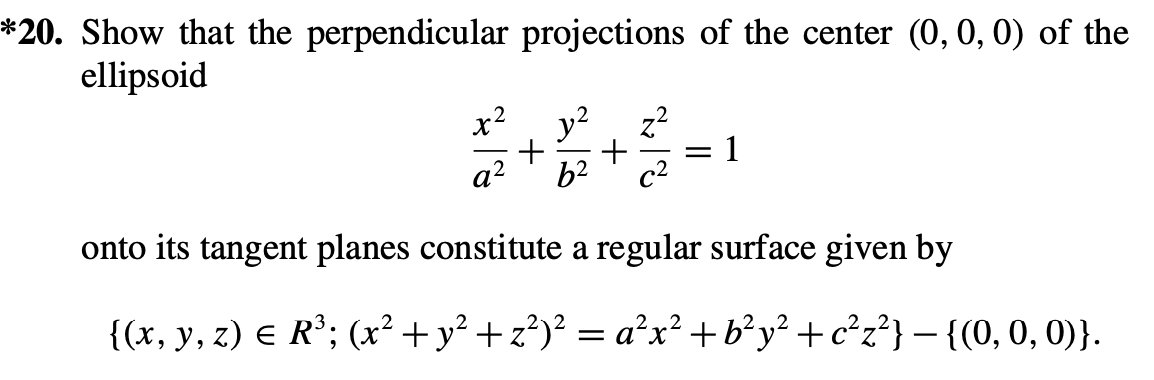
\includegraphics[height=10cm,width=18cm]{hwextra}
\end{question}
\begin{proof}
Let $S$ be the ellipsoid. Let 
\begin{align*}
E\triangleq  \set{(x,y,z)\inr^3 : (x^2+y^2+z^2)^2=a^2x^2+b^2y^2+c^2z^2}\setminus O
\end{align*}
Let $E'$ be the perpendicular projections of  $O$ of $S$ onto the tangent planes of  $S$. We are required to prove 
 \begin{align*}
   \vi{E'=E}
\end{align*}
We first prove 
\begin{align*}
\blue{E' \subseteq E}
\end{align*}


Fix $p_0=(x_0,y_0,z_0)\in S$. We first prove 
\begin{align}
\label{tp0}
\olive{T_{p_0}(S)=\set{(x,y,z)\inr^3: \frac{xx_0}{a^2}+\frac{yy_0}{b^2}+\frac{zz_0}{c^2}=1}}
\end{align}
Fix 
\begin{align*}
f(x,y,z)=\frac{x^2}{a^2}+\frac{y^2}{b^2}+\frac{z^2}{c^2}
\end{align*}
We have $S=f^{-1}(1)$. Compute 
\begin{align*}
\nabla f(x,y,z)=(\frac{2x}{a^2},\frac{2y}{b^2},\frac{2z}{c^2})
\end{align*}
Then because $T_{p_0}(S)\perp \nabla f(p_0)$, we have 
\begin{align*}
T_{p_0}(S)=\set{(x,y,z)\inr^3: \frac{x x_0}{a^2}+\frac{y y_0}{b^2}+\frac{z z_0}{c^2}=\frac{x_0^2}{a^2}+\frac{y_0^2}{b^2}+\frac{z_0^2}{c^2}=1}\odone
\end{align*}
We know that the line $L$ passing through $O$ and perpendicular to $T_{p_0}(S)$ can be parametrized by 
\begin{align*}
  L(t)=t\nabla f(p_0)\equiv t(\frac{x_0}{a^2},\frac{y_0}{b^2},\frac{z_0}{c^2})
\end{align*}
Compute 
\begin{align*}
L(t)\in T_{p_0}(S)\implies t(\frac{x_0^2}{a^4}+\frac{y_0^2}{b^4}+\frac{z_0^2}{c^4})=1
\end{align*}
This implies 
\begin{align*}
t=(\frac{x_0^2}{a^4}+\frac{y_0^2}{b^4}+\frac{z_0^2}{c^4})^{-1}\text{ and }q=t(\frac{x_0}{a^2},\frac{y_0}{b^2},\frac{z_0}{c^2})
\end{align*}
where $q\in T_{p_0}(S)$ is the point to which $O$ is perpendicular projected.\\ 

Express $q=(x,y,z)$. Now, we can reduce the problem into proving 
\begin{align*}
\blue{(x^2+y^2+z^2)^2=a^2x^2+b^2y^2+c^2z^2}
\end{align*}



Compute  
\begin{align*}
  (x^2+y^2+z^2)^2=\Big(t^2(\frac{x_0^2}{a^4}+\frac{y_0^2}{b^4}+\frac{z_0^2}{c^2}) \Big)^2
\end{align*}
Compute 
\begin{align*}
a^2x^2+b^2y^2+c^2z^2=t^2 (\frac{x_0^2}{a^2}+\frac{y_0^2}{b^2}+\frac{z_0^2}{c^2})=t^2\hspace{0.5cm}(\because \frac{x_0^2}{a^2}+\frac{y_0^2}{b^2}+\frac{z_0^2}{c^2}=1)
\end{align*}
We reduce the problem into proving
\begin{align*}
\blue{t^2 (\frac{x_0^2}{a^4}+\frac{y_0^2}{b^4}+\frac{z_0^2}{c^4})^2=1}
\end{align*}
Note that $t=(\frac{x_0^2}{a^4}+\frac{y_0^2}{b^4}+\frac{z_0^2}{c^4})^{-1}$ and we are done. $\bdone$ \\

It remains to prove 
\begin{align*}
\vi{E\subseteq E'}
\end{align*}
Fix $(x_1,y_1,z_1)\in S_1$. Let
\begin{align*}
r\triangleq \sqrt{a^2x_1^2+b^2y_1^2+c^2z_1^2} 
\end{align*}
We claim 
\begin{align*}
\vi{(x_1,y_1,z_1)\text{ is the projection of $O$ onto the tangent plane of  $S$ at  $(\frac{a^2x_1}{r},\frac{b^2y_1}{r},\frac{c^2z_1}{r})$ }}
\end{align*}
It is easily checked that $(\frac{a^2x_1}{r},\frac{b^2y_1}{r},\frac{c^2z_1}{r})\in S$. Let $p=(\frac{a^2x_1}{r},\frac{b^2y_1}{r},\frac{c^2z_1}{r})$. Using (\myref{}{tp0}), we have 
\begin{align*}
T_p(S)=\set{(x,y,z)\inr^3 : \frac{x x_1+y y_1+z z_1}{r}=1}
\end{align*}
It is now very clear that 
\begin{align*}
  (x_1,y_1,z_1)\text{ as a vector is perepndicular to $T_p(S)$ }
\end{align*}
and we can use the fact $(x_1,y_1,z_1)\in E$ to compute 
\begin{align*}
\frac{x_1^2+y_1^2+z_1^2}{r}= \frac{\sqrt{a^2x_1^2+b^2y_1^2+c^2z_1^2} }{r}=1
\end{align*}
This conclude $(x_1,y_1,z_1)\in T_p(S)$. $\vdone$
\end{proof}
\begin{question}{}{}
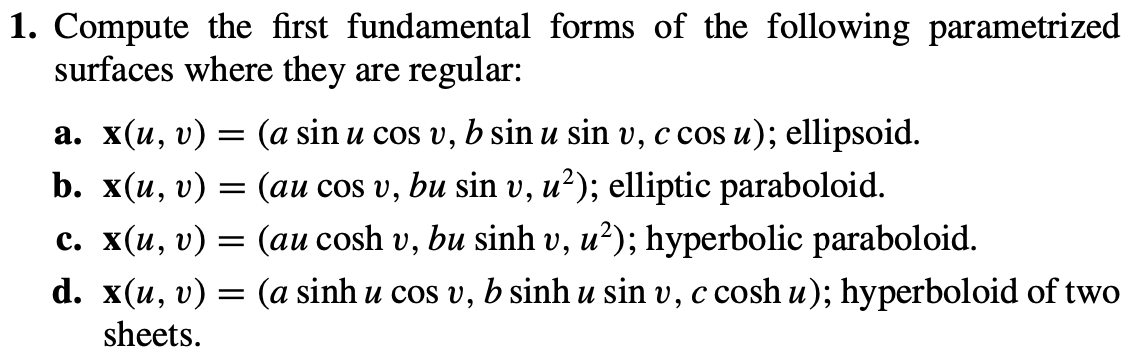
\includegraphics[height=10cm,width=18cm]{hw4q8}
\end{question}
\begin{proof}
Let $\alpha '(0)\in T_p(S)$ and express $\alpha (t)=\textbf{x}(u(t),v(t))$. We have 
\begin{align*}
I_p(\alpha '(0))&= \alpha '(0)\cdot \alpha '(0)\\
&= \Big( u'(0)\partial_u \textbf{x}(p)+ v'(0)\partial_u \textbf{x}(p) \Big) \cdot\Big( u'(0)\partial_u \textbf{x}(p)+ v'(0)\partial_u \textbf{x}(p) \Big)\\
&= \abso{\textbf{x}_u(p)}^2 (u'(0))^2+ 2(\partial_u \textbf{x}(p)\cdot \partial_v \textbf{x}(p))u'(0)v'(0)+ \abso{\textbf{x}_v(p)}^2 (v'(0))^2\\
&\triangleq E(u'(0))^2 +2Fu'(0)v'(0)+G(v'(0))^2
\end{align*}
From now on, we compute only $E,F,G$.\\


\textbf{(a)}
Compute 
\begin{align*}
&\partial_u \textbf{x}=(a\cos u \cos v, b \cos u \sin v, -c \sin u)\\
\text{ and }&\partial_v \textbf{x}=(-a \sin u \sin v,b \sin u \cos v, 0)
\end{align*}
This give us 
\begin{align*}
E&=\abso{\partial_u\textbf{x}}^2= \cos^2 u (a^2\cos ^2v + b^2 \sin^2 v)+c^2 \sin^2 u \\
F&=\partial_u \textbf{x}\cdot \partial_v \textbf{x}=(-a^2+b^2)\cos u \sin u \cos v \sin v\\
G&=\abso{\partial_v \textbf{x}}^2= \sin^2 u (a^2 \sin^2 v + b^2 \cos ^2 v)
\end{align*}
\textbf{(b)} Compute 
\begin{align*}
\partial_u \textbf{x}=(a\cos v, b \sin v, 2u)\text{ and }\partial_v \textbf{x}=(-au \sin v, b u \cos v, 0)
\end{align*}
This give us 
\begin{align*}
E&=\abso{\partial_u \textbf{x}}^2= a^2 \cos^2 v + b^2 \sin^2 v + 4u^2\\
F&=\partial_u \textbf{x}\cdot \partial_v \textbf{x}=\cos v \sin v (-a^2 +b^2)u\\
G&=\abso{\partial_v \textbf{x}}^2 = u^2 (a^2 \sin^2 v+ b^2 \cos ^2 v)
\end{align*}
\textbf{(c)} Compute 
\begin{align*}
  \partial_u \textbf{x}=(a \cosh v, b \sinh v,2u)\text{ and }\partial_v \textbf{x}=(au \sinh v, b u \cosh v, 0)
\end{align*}
This give us 
\begin{align*}
E&=\abso{\partial_u \textbf{x}}^2 = a^2 \cosh^2 v+ b^2 \sinh^2 v+4u^2\\
F&=\partial_u \textbf{x}\cdot \partial_v \textbf{x}=(a^2+b^2)u \cosh v \sinh v\\
G&=\abso{\partial_v \textbf{x}}^2= u^2 (a^2 \sinh^2 v+ b^2 \cosh^2 v)
\end{align*}
\textbf{(d)} Compute 
\begin{align*}
\partial_u \textbf{x}=(a \cosh u \cos v , b \cosh u \sin v, c\sinh u)\text{ and }\partial_v \textbf{x}=(-a\sinh u \sin v, b \sinh u \cos v, 0)
\end{align*}
This give us 
\begin{align*}
E&= \abso{\partial _u\textbf{x}}^2= \cosh^2 u (a^2 \cos^2 v+b^2 \sin^2 v)+c^2 \sinh^2 u\\
F&=\partial_u \textbf{x}\cdot \partial_v \textbf{x}= \cosh u \sinh u \cos v \sin v (b^2-a^2)\\
G&=\abso{\partial_v \textbf{x}}^2 = \sinh^2 u (a^2 \sin^2 v +b^2 \cos^2 v)
\end{align*}
\end{proof}
\begin{question}{}{}
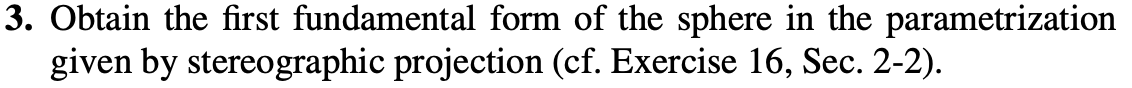
\includegraphics[height=3cm,width=18cm]{hw4q9}
\end{question}
\begin{proof}
We are given 
\begin{align*}
\textbf{x}(u,v)=\Big(\frac{4u}{u^2+v^2+4}, \frac{4v}{u^2+v^2+4}, \frac{2(u^2+v^2)}{u^2+v^2+4} \Big)
\end{align*}
Note that in Question 2.5.1, we have already given the complete formula of $I_p(\alpha '(0))$. We only have to compute $E,F,G$. 
\begin{align*}
\partial_u \textbf{x}&=\Big(\frac{4(-u^2+v^2+4)}{(u^2+v^2+4)^2}, \frac{-8vu}{(u^2+v^2+4)^2}, \frac{16u}{(u^2+v^2+4)^2} \Big)\\
\partial_v \textbf{x}&=\Big(\frac{-8uv}{(u^2+v^2+4)^2}, \frac{4(-v^2+u^2+4)}{(u^2+v^2+4)^2},\frac{16v}{(u^2+v^2+4)^2} \Big)
\end{align*}
Then compute 
\begin{align*}
E&= \frac{16u^4+32u^2v^2+128u^2+16v^4+128v^2+256}{(u^2+v^2+4)^4}\\
F&=0\\
G&= \frac{16 v^4 + 32u^2v^2+ 128 v^2 + 16u^4 + 128 u^2 +256}{(u^2+v^2+4)^4}
\end{align*}
\end{proof}
\begin{question}{}{}
\includegraphics[height=7cm,width=18cm]{hw4q10}
\end{question}
\begin{proof}
For each $v$, define 
\begin{align*}
\alpha_v (t)=\textbf{x}(t,v)
\end{align*}
 WOLG, we are require to show  
\begin{align*}
  \vi{\forall r\inr^+,\int_0^r \abso{\alpha'_v(t)}dt\text{ is a constant in $v$ }\iff \frac{\partial E}{\partial v}=0}
\end{align*}
$(\longleftarrow)$\\

Note that we have 
\begin{align*}
u'(t)=1 \text{ and }v'(t)=0\text{ if we write }\alpha _v(t)=\textbf{x}(u(t),v(t))
\end{align*}
Then, we have 
\begin{align*}
\int_0^C \abso{\alpha'_v(t)}dt=\int_0^C \sqrt{E(t,v)}dt
\end{align*}
If $ \frac{\partial E}{\partial v}=0$, then for each $v_1,v_2$, we clearly have  
 \begin{align*}
\int_0^r \abso{\alpha '_{v_1}(t)}dt=\int_0^r\sqrt{E(t,v_1)}dt=\int_0^r \sqrt{E(t,v_2)}dt=\int_0^r \abso{\alpha '_{v_2}(t)}dt
\end{align*}
$(\longrightarrow)$\\

Suppose for all $r\inr^+$, the function $\int_0^r \abso{\alpha '_v(t)}dt$ is a constant in $v$. We then can define  $f:\R^+\rightarrow \R^+$ by 
\begin{align*}
f(r)=\int_0^r \abso{\alpha '_v(t)}dt\text{ for all $v$ }
\end{align*}
Differentiating $f$, we see 
 \begin{align*}
f'(r)=\sqrt{E(r,v)} \text{ for all $v$ }
\end{align*}
This tell us 
\begin{align*}
E(r,v)\text{ is a constant in $v$ for all $r$ }
\end{align*}
which implies 
\begin{align*}
\frac{\partial E}{\partial v}=0\vdone
\end{align*}






\end{proof}
\begin{question}{}{}
\includegraphics[height=7cm,width=18cm]{hw4q11}
\end{question}
\begin{proof}
Note that $\frac{\partial  E}{\partial v}=\frac{\partial G}{\partial u}=0$ implies 
\begin{align*}
E\text{ stay constant in $v$ and  $G$ stay constant in  $u$ }
\end{align*}
In other words, $E$ can be treated as a function of  $u$ and $G$ can be treated as a function of $v$. Let
\begin{align*}
\overline{u}(u)=\int_0^u  \sqrt{E(t)}dt \text{ and }\overline{v}(v)=\int_0^v \sqrt{G(t)}dt 
\end{align*}
Reparametrize by 
\begin{align*}
\textbf{x}(u(\overline{u}),v(\overline{v}))
\end{align*}
By Chain Rule and Single-Variable Inverse Function Theorem, we have 
\begin{align*}
\partial_{\overline{u}} \textbf{x}=\frac{1}{\sqrt{E(u)} }\partial_u \textbf{x} \text{ and }\partial_{\overline{v}}\textbf{x}=\frac{1}{\sqrt{G(v)} }\partial_v \textbf{x}
\end{align*}
This give us 
\begin{align*}
  \overline{E}= \partial_{\overline{u}}\textbf{x}\cdot \partial_{\overline{u}}\textbf{x}= \frac{E(u)}{E(u)}=1\text{ and }\overline{G}=\partial_{\overline{v}}\textbf{x}\cdot \partial_{\overline{v}}\textbf{x}=\frac{G(v)}{G(v)}=1
\end{align*}
Now, by CS-inequality, we know $\overline{F}=\partial_{\overline{u}}\textbf{x}\cdot \partial_{\overline{v}}\textbf{x}\in (-1,1)$. Then there must exists $\theta$ such that $\overline{F}=\cos \theta$. 
\end{proof}
\begin{question}{}{}
\includegraphics[height=7cm,width=18cm]{hw4q12}
\end{question}
\begin{proof}
\textbf{(a)}\\

Because $S$ is a surface of revolution, we have an almost global chart 
\begin{align*}
\textbf{x}(\theta,s)=(\cos \theta f(s),\sin \theta f(s),g(s))
\end{align*}
where 
\begin{align*}
f(s)=\rho(s)\text{ and }(f')^2+(g')^2=1
\end{align*}
Compute 
\begin{align*}
\partial_\theta \textbf{x}=(-\sin \theta f(s), \cos \theta f(s),0)\text{ and }\partial_s \textbf{x}=(\cos \theta f'(s),\sin \theta f'(s),g'(s))
\end{align*}
This let us compute 
\begin{align*}
E&=\abso{\partial _\theta \textbf{x}}^2=\abso{f(s)}^2=\rho(s)^2 \\
F&=\partial_\theta \textbf{x}\cdot \partial_ s \textbf{x}=0 \\
G&=\abso{\partial_s \textbf{x}}^2 = (f'(s))^2 + (g'(s))^2=1
\end{align*}
Now we see that the area $A(S)$ of $S$ is exactly 
\begin{align*}
A(S)=\int_0^{2\pi}\int_0^l \sqrt{EG-F^2}dsd\theta =2\pi \int_0^l \rho (s) ds
\end{align*}
\textbf{(b)}\\
Note that 
\begin{align*}
  \big(f(s),g(s) \big)\triangleq (a+r \cos \frac{s}{r},a+ r \sin \frac{s}{r})\text{ where }f(s)\equiv \rho(s)
\end{align*}
satisfy all the condition. Then we can compute the surface area of the torus by
\begin{align*}
2\pi \int_0^{2\pi r} (a+ r \cos (\frac{s}{r}))ds= 4\pi^2 ra
\end{align*}

\end{proof}
\begin{question}{}{}
\includegraphics[height=18cm,width=18cm]{hw4q13}
\end{question}
\begin{proof}
\textbf{(a)}\\

Suppose $\nabla f= \frac{f_uG-f_vF}{EG-F^2}\textbf{x}_u+ \frac{f_vE-f_uF}{EG-F^2}$. First observe 
\begin{align*}
\langle \nabla f, \textbf{x}_u\rangle &= \frac{f_u G -f_v F}{EG-F^2} E+ \frac{f_v E-f_u F}{EG-F^2}F\\
&=\frac{f_u(GE-F^2)}{EG-F^2}\\
&=f_u=\frac{\partial }{\partial u}(f \circ \textbf{x})=df(\textbf{x}_u)
\end{align*}
The justification of the last inequality is as followed. Define 
\begin{align*}
\alpha (t)=\textbf{x}(u_0+t,v_0)
\end{align*}
We have 
\begin{align*}
\alpha (0)=\textbf{x}(u_0,v_0)\text{ and }\alpha '(0)=d\textbf{x}_{(u_0,v_0)}(1,0)=\textbf{x}_u(u_0,v_0)
\end{align*}
Now
\begin{align*}
df_{\textbf{x}(u_0,v_0)}(\textbf{x}_u(u_0,v_0))\overset{\text{def}}{=}\frac{d}{dt}(f\circ \alpha (t))\Big|_{t=0}=\frac{d}{dt}\big((f\circ \textbf{x})(u_0+t,v_0)\big)=\frac{\partial}{\partial u}(f\circ \textbf{x})(u_0,v_0)
\end{align*}
This justified the $\langle \nabla f, \textbf{x}_u\rangle =df(\textbf{x}_u)$.\\

Similarly, we have 
\begin{align*}
\langle \nabla f,\textbf{x}_v\rangle =df(\textbf{x}_v)
\end{align*}
Now, for all $w\in T_p(S)$, we see that 
\begin{align*}
\langle \nabla f(p),w\rangle&= \langle \nabla f(p),c_u\textbf{x}_u(p)+c_v\textbf{x}_v(p)\rangle\hspace{0.5cm}(\text{ for a unique pair $c_u,c_v\inr$ })\\
&=c_u\langle \nabla f(p),\textbf{x}_u(p)\rangle + c_v \langle \nabla f(p),\textbf{x}_v(p)\rangle \\
&=c_u df_p(\textbf{x}_u(p))+c_vdf_p(\textbf{x}_v(p))\\
&=df_p(c_u\textbf{x}_u(p)+c_v\textbf{x}_v(p))=df_p(w)
\end{align*}
If $S=\R^2$ with coordinates  $x,y$, we can easily compute 
 \begin{align*}
\textbf{x}_x=(1,0)\text{ and }\textbf{x}_y=(0,1)
\end{align*}
and 
\begin{align*}
E=1\text{ and }F=0\text{ and }G=1
\end{align*}
Then from the formula of $\nabla f$ we just derived, we have 
\begin{align*}
\nabla f= f_x(1,0)+f_y(0,1)\equiv f_xe_1+f_ye_2
\end{align*}
\textbf{(b)}\\

By C-S inequality, we see that 
\begin{align*}
 df_p(v)\equiv \langle \nabla f(p),v\rangle \text{ reach maximum if and only if  $v=c_0\nabla f(p)$  for some positive $c_0$ }
\end{align*}
It then come very clear, under the constraint $\abso{v}=1$, that $c_0$ must be  $\frac{1}{\abso{\nabla f(p)}}$.\\

\textbf{(c)}\\

Let that constant be $c_0$, and let $p=\textbf{x}(q) \in C$. Define $g:\R^{2+1} \rightarrow \R$ by 
\begin{align*}
g(u,v,t)=f(\textbf{x}(u,v))-t
\end{align*}
Check that 
\begin{align*}
\partial_t g=-1 \neq 0
\end{align*}
Then by Implicit function theorem, there exists a function $h:U\subseteq \R^2 \rightarrow \R$ such that 
\begin{align*}
h(q)=c_0 \text{ and }g(u,v,h(u,v))=0\text{ for all $(u,v)\in U$ }
\end{align*}
We now see 
\begin{align*}
C=(h\circ \textbf{x}^{-1})^{-1}(c_0)\text{ which is a regular preimage }
\end{align*}
This established that $C$ is a regular curve.\\

Locally parametrize $\gamma (t)\subseteq C$. Because $f\circ \gamma $ stay constant, we see
\begin{align*}
0=df_{\gamma (t)}(\gamma '(t))=\langle \nabla f(\gamma (t)),\gamma '(t)\rangle 
\end{align*}
This then implies $\nabla f(\gamma (t))$ is perpendicular to $\gamma '(t)$, thus perpendicualr to $C$. 
\end{proof}
\chapter{Gauss Map}
\section{Equivalent Definitions of the Term "Orientable"}
\begin{mdframed}
Only three results are important in this section 
\begin{enumerate}[label=(\alph*)]
  \item \myref{Definition}{SD}
  \item Preimage of regular value is orientable. (\myref{Theorem}{PoaR})
  \item The Gauss Map $N:S\rightarrow \R^3$ maps $S$ into  $S^2$ because  $N(p)$ is unit for all $p\in  S$, and because $T_pS\perp N(p)\perp T_{N(p)}S^2$, we see $T_{N(p)}S^2=T_pS$, so one can just treat the derivative of $dN_p:T_{p}S\rightarrow T_{N(p)}S^2$ as a linear transformation $dN_p:T_pS\rightarrow T_pS$ that maps $T_pS$ into itself. 
\end{enumerate}
Particularly, \myref{Theorem}{PoaR} give a simple proof that $S^2$ is orientable, and perhaps almost all questions in midterm 2 that ask you to show some regular surface is orientable can be very easily answered using \myref{Theorem}{PoaR}.
\end{mdframed}
\begin{mdframed}
In this section, by an \textbf{atlas} of a regular surface $S$, we mean a set $L$ of parametrizatoin
 \begin{align*}
L=\set{\textbf{x}_\ld  :U_\ld  \rightarrow S|\ld  \in \Lambda }
\end{align*}
such that  $L$ cover  $S$ 
 \begin{align*}
S\subseteq \bigcup_{\textbf{x}_\ld \in L} \textbf{x}_\ld  (U_\ld ) 
\end{align*}
\end{mdframed}
\begin{definition}
\label{FD}
\textbf{(First Definition: Consistently Oriented Atlas)} We say $S$ is orientable if $S$ has at least one  \textbf{consistently oriented atlas} $L$.\\



We say an atlas $L$ of  $S$ is consistently orietned if every two  $\textbf{x}(u,v),\overline{\textbf{x}}(\overline{u},\overline{v})$ that belongs $L$ and has non-empty intersection $E$ satisfy 
\begin{align*}
  \text{det}\Big([df_{(u,v)}]\Big)>0\text{ for all $(u,v) \in \textbf{x}^{-1}(E)$ }
\end{align*}
where the function $f$ from $\textbf{x}^{-1}(E)$ to $(\overline{\textbf{x}})^{-1}(E)$ is defined by 
\begin{align*}
f(u,v)\triangleq (\overline{\textbf{x}})^{-1}\circ \textbf{x}(u,v)
\end{align*}
\end{definition}
\begin{definition}
\label{SD}
\textbf{(Second Definition: Gauss Map)} We say $S$ is orientable if there exists a differentiable function $N$, which we call \textbf{Gauss map}, that maps each $p\in  S$ to a unit vector $N(p)\inr^3$ such that 
\begin{align*}
N(p)\perp T_p(S)
\end{align*}
\end{definition}
\begin{mdframed}
Note that in \myref{Definition}{FD}, $[df]$ is just
 \begin{align*}
[df]= \frac{\partial (\overline{u},\overline{v})}{\partial (u,v)}
\end{align*}
You will later use this fact. 
\end{mdframed}
\begin{theorem}
\textbf{(Equivalence of \myref{Definition}{FD} and \myref{Definition}{SD})}  
\end{theorem}
\begin{proof}
Suppose $S$ has an consistently oriented atlas  $L$. We are required to 
 \begin{align*}
\vi{\text{ define an $N:S\rightarrow \R^3$ that satisfy \myref{Definition}{SD}}}
\end{align*}
For each $p \in S$, arbitrarily pick a chart $\textbf{x}\in L$ covering $p$. We claim
\begin{align*}
  \vi{N(p)\triangleq \Big(\frac{\textbf{x}_u\times \textbf{x}_v}{\abso{\textbf{x}_u \times \textbf{x}_v}} \Big)(p)\text{ suffices }}
\end{align*}
We are required to show 
\begin{enumerate}[label=(\alph*)]
  \item \vi{$N$ is well defined}
  \item \vi{$N$ is differentiable}
  \item  $\forall p \in S, \abso{N(p)}=1$ 
\end{enumerate}
It is easy to check (c). That's why (c) isn't colored.\\

Suppose $\overline{\textbf{x}}\in L$ cover $p$. To show $N$ is well defined, we have to show 
\begin{align*}
\vi{\big(\overline{\textbf{x}}_{\overline{u}}\times \overline{\textbf{x}}_{\overline{v}} \big)(p)=c\big((\textbf{x}_u \times \textbf{x}_v) \big)(p) \text{ for some $c\inr^+$ }}
\end{align*}
Calculus 2 taught us (You shall blindly assume this is correct.)
\begin{align}
\label{CTYb}
\overline{\textbf{x}}_{\overline{u}}\times \overline{\textbf{x}}_{\overline{v}}= \big(\textbf{x}_u \times \textbf{x}_v \big) \text{det}\Big(\frac{\partial  (u,v)}{\partial (\overline{u},\overline{v})} \Big) 
\end{align}
Note that the \myref{Definition}{FD} says $\text{det}\Big(\frac{\partial  (u,v)}{\partial (\overline{u},\overline{v})} \Big) $ is positive at $p$ (in fact every where the two chart $\textbf{x},\overline{\textbf{x}}$ intersect). This complete the proof of  (a).\\

Fix $p\in  S$. To show $N$ is differentiable at $p$, we are required to show there exists $\textbf{x}$ covering $p$ such that 
\begin{align*}
  \vi{N\circ \textbf{x}:U\subseteq\R^2 \rightarrow \R^3\text{ is differentiable }}
\end{align*}
This shall be clear once we write down the exact expression of $N\circ \textbf{x}$
\begin{align*}
\text{ for all $(u_0,v_0)\in U$ we have }N\circ \textbf{x}(u_0,v_0)= \frac{\frac{\partial \textbf{x} }{\partial u}(u_0,v_0)\times \frac{\partial \textbf{x}}{\partial v}(u_0,v_0)}{\abso{\frac{\partial \textbf{x} }{\partial u}(u_0,v_0)\times \frac{\partial \textbf{x}}{\partial v}(u_0,v_0)}}
\end{align*}
This is clearly differnetiable. $\vdone$ \\

Now, given a differtiable unit normal vector field $N:S\rightarrow \R^3$, we are required 
\begin{align*}
\blue{\text{ to construct a consistently oriented atlas }L}
\end{align*}
Note that given a chart $\textbf{x}(u,v):U\rightarrow S$ containing $p$, if we define 
\begin{align*}
E\triangleq \set{(x,y)\inr^2: (y,x)\in U}
\end{align*}
(It is easy to see $E$ is open by using the fact $U$ is open) and define $\textbf{x}':E\rightarrow S$ by 
\begin{align*}
\textbf{x}'(u,v)\triangleq \textbf{x}(v,u)
\end{align*}
we have 
\begin{align*}
\textbf{x}'_u\times \textbf{x}'_v= \textbf{x}_v\times \textbf{x}_u = -(\textbf{x}_u \times \textbf{x}_v)
\end{align*}
It is clear that there exists an atlas $L$ contained only connected charts. We can now use  $\textbf{x}'$ to replace the $\textbf{x}$ that has the wrong direction, i.e. 
\begin{align*}
\frac{\textbf{x}_u\times \textbf{x}_v}{\abso{\textbf{x}_u \times \textbf{x}_v}}(p)=-N(p)
\end{align*}
and have an atlas $L'$ that always give us the correct direction.
\begin{mdframed}
Note that there is a reason we require $L$ to contain only connected charts, since if $\textbf{x}(U)$ is disconnected for some $\textbf{x}$, it is possible  
\begin{align*}
\frac{\textbf{x}_u \times \textbf{x}_v}{\abso{\textbf{x}_u \times \textbf{x}_v}}(u_0,v_0)=N(\textbf{x}(u_0,v_0))\text{ and }\frac{\textbf{x}_u \times \textbf{x}_v}{\abso{\textbf{x}_u \times \textbf{x}_v}}(u_1,v_1)=-N(\textbf{x}(u_1,v_1))
\end{align*}
which invalidate the whole proof.
\end{mdframed}
The fact that all charts in $L'$ has the same direction can now let us easily use \myref{Equation}{CTYb} to verify 
 \begin{align*}
\text{det}\Big(\frac{\partial  (u,v)}{\partial (\overline{u},\overline{v})} \Big) >0 \bdone
\end{align*}
\end{proof}
\begin{theorem}
\label{PoaR}
\textbf{(Preimage of a Regular Value is orientible)} If $f:\R^3\rightarrow \R$ is a smooth function and $r\inr$ is a regular value of $f$, then 
 \begin{align*}
f^{-1}(r)\text{ is an orientable regular surface }
\end{align*}
\end{theorem}
\begin{proof}
We claim 
\begin{align*}
\vi{N(p)\triangleq \frac{\nabla f(p)}{\abso{\nabla f(p)}}\text{ suffices }}
\end{align*}
The fact $\nabla f(p)\perp T_pS$ is proved in the last Midterm. The trick is let $\alpha $ be a curve that lies in $S\triangleq f^{-1}(r)$, and see 
\begin{align*}
0=(f\circ \alpha )'(s)=\nabla f(\alpha (s))\cdot \alpha '(s)
\end{align*}
Express $N(p)$ precisely,  
\begin{align*}
N(x_0,y_0,z_0)= \Big(\frac{f_x}{\sqrt{f_x^2+f_y^2+f_z^2} }, \frac{f_y}{\sqrt{f_x^2+f_y^2+f_z^2} }, \frac{f_z}{\sqrt{f_x^2+f_y^2+f_z^2} } \Big)\Big|_{p=(x_0,y_0,z_0)}
\end{align*}
It is then clear that $N:S\rightarrow \R^3$ is a restriction of the differentiable function $\frac{\nabla f}{\abso{\nabla f}}$. Use the fact $f$ is smooth to show $\frac{\nabla f}{\abso{\nabla f}}$ is differentiable. This implies $N$ is differentiable. 
\end{proof} 
\begin{mdframed}
Reminder: If a function $f:S\rightarrow \R^3$ is the restriction of some differentiable function $g:\R^3\rightarrow \R$, then $f$ is differentiable. This can be directly proved using Chain Rule. 
\end{mdframed}
\section{Second Fundamental Form}
\begin{mdframed}
  Given an inner product space $\Big(V, \langle \cdot,\cdot\rangle  \Big)$, we say a linear transformation $T\in L(V,V)$ is \textbf{self-adjoint} if 
\begin{align*}
\langle Tv,w\rangle = \langle v,Tw\rangle \text{ for all $v,w\in V$ }
\end{align*}
\end{mdframed}
\begin{definition}
  \textbf{(Definition of Second Fundamental Form)} We define the second fundamental form $\Sec_p(v):T_pS\rightarrow R$ on each point $p$ of $S$ by  
\begin{align*}
\Sec _p(v)\triangleq - \langle dN_p(v),v\rangle 
\end{align*}
\end{definition}
\begin{mdframed}
We will later show $dN_p:T_pS\rightarrow T_pS$ is self-adjoint. This then implies that $\Sec_p$ is a quadratic form.
\end{mdframed}
\begin{definition}
\textbf{(Definition of Normal Curvature)} Given a curve $\alpha (s)$ that lies in $S$ passing through $p=\alpha (0)$, let $\kappa$ be the curvature of $C$ at $p$, and let  
\begin{align*}
\cos \theta \triangleq \langle N_\alpha (p),N(p)\rangle 
\end{align*}
The normal curvature $\kappa_{\alpha ,p}$ of $\alpha (s)$ at $p$ is then defined by 
\begin{align*}
\kappa_{\alpha ,p} \triangleq  \kappa \langle N_\alpha (p),N(p)\rangle = \kappa \cos \theta
\end{align*}
\end{definition}
\begin{theorem}
\label{Ncdo}
\textbf{(Normal curvature depends only on $\alpha '(0)$)} Suppose we are given a curve $\alpha (s)$  that lies in $S$ passing through $p$.  We have 
\begin{align*}
\kappa_{\alpha ,p }=\Sec_p(\alpha '(0))
\end{align*}
\end{theorem}
\begin{proof}
By definition, we have 
\begin{align*}
\langle N(\alpha (s)),\alpha '(s)\rangle =0\text{ for all $s$ }
\end{align*}
Taking Differentiation
\begin{align*}
\langle N(\alpha (s)),\alpha ''(s)\rangle + \langle dN_{\alpha (s)}(\alpha '(s)), \alpha '(s)\rangle =0 
\end{align*}
This give us 
\begin{align*}
\Sec_{\alpha (s)}(\alpha '(s))= \langle N(\alpha (s)),\alpha ''(s)\rangle 
\end{align*}
Especially, let $s=0$, we have 
\begin{align*}
\Sec_p(\alpha '(0))=\langle N(p),\kappa N_\alpha (p)\rangle = \kappa \langle N_\alpha (p),N(p)\rangle = \kappa_{\alpha,p }
\end{align*}
\end{proof}
\begin{mdframed}
One thing about \myref{Theorem}{Ncdo} is that it show us that give two curve $\alpha (s),\beta (s)$ passing though $p=\alpha (0)=\beta (0)$, if two curves has the same tangent at $0$, i.e. 
 \begin{align*}
\alpha '(0)=\beta '(0)
\end{align*}
then we have 
\begin{align*}
\kappa_{\alpha ,p}=\Sec_p (\alpha '(0))=\Sec_p (\beta '(0))=\kappa_{\beta ,p}
\end{align*}
\end{mdframed}
\begin{theorem}
\textbf{($dN_p$ is self-adjoint)} Given a $p\in  S$, the linear transformation $dN_p:T_p(S)\rightarrow T_{N(p)}(S^2)$ is self-adjoint.
\end{theorem}
\begin{proof}
We first prove 
\begin{align*}
\vi{\langle dN_p(\textbf{x}_u),\textbf{x}_v\rangle = \langle \textbf{x}_u , dN_p (\textbf{x}_v)\rangle }
\end{align*}
Note that 
\begin{align*}
\langle N \circ \textbf{x},\textbf{x}_u\rangle = \langle N\circ \textbf{x},\textbf{x}_v\rangle = 0\text{ on  $U$ }
\end{align*}
Respectively take partial derivative with respect to $v,u$, we have 
 \begin{align*}
\langle dN_p(\textbf{x}_v),\textbf{x}_u\rangle + \langle N\circ \textbf{x}, \textbf{x}_{uv}\rangle = \langle dN_p(\textbf{x}_u),\textbf{x}_v\rangle + \langle N\circ \textbf{x}, \textbf{x}_{vu}\rangle =0 \text{ on $U$ where  $p=\textbf{x}(u,v)$ }
\end{align*}
Note that $\textbf{x}_{vu}=\textbf{x}_{uv}$ and we are done. $\vdone$\\

Observe 
\begin{align}
&\langle dN_p(c_1\textbf{x}_u +c_2 \textbf{x}_v),c_3\textbf{x}_u+c_4\textbf{x}_v\rangle \notag\\
&=c_1c_3 \langle dN_p(\textbf{x}_u),\textbf{x}_u\rangle + c_2c_4 \langle dN_p(\textbf{x}_v),\textbf{x}_v\rangle + c_1c_4\langle dN_p(\textbf{x}_u), \textbf{x}_v\rangle + c_2c_3 \langle dN_p(\textbf{x}_v),\textbf{x}_u\rangle \notag  \\
&=c_1c_3 \langle dN_p(\textbf{x}_u),\textbf{x}_u\rangle + c_2c_4 \langle dN_p(\textbf{x}_v),\textbf{x}_v\rangle + (c_1c_4+c_2c_3)\langle dN_p(\textbf{x}_u),\textbf{x}_v\rangle \label{xuv} \\
&=\langle c_1\textbf{x}_u+c_2\textbf{x}_v, dN_p(c_3\textbf{x}_u+c_4\textbf{x}_v)\rangle \label{xuv2}
\end{align}
Note that \myref{Equation}{xuv} and \myref{Equation}{xuv2} use the \vi{violet} result, and note that \myref{Equation}{xuv2} implies that $dN_p$ is self-adjoint. 
\end{proof}
\begin{mdframed}
Because $dN_p:T_p(S)\rightarrow T_p(S)$ is self-adjoint, by spectral theorem, we know there exists an orthonormal basis $\set{e_1,e_2}$ of $T_pS$ containing only eigenvectors. Express 
\begin{align*}
  dN_p(e_1)=-\kappa_1 e_1\text{ and }dN_p(e_2)=-\kappa _2 e_2\text{ and }\kappa_1 \geq \kappa_2
\end{align*}
We say $\kappa_1,\kappa_2$ are the \textbf{principal curvature of $p$ at  $S$} and $e_1,e_2$ are the  \textbf{principal direction of $p$ at  $S$}.\\




Note that we have  
\begin{align*}
\Sec_p(c_1e_1+c_2e_2)&=-dN_p(c_1e_1+c_2e_2)\cdot (c_1e_1+c_2e_2)\\
&=-(-c_1\kappa_1 e_1-c_2\kappa_2 e_2)\cdot (c_1e_1+c_2e_2)\\
&=c_1^2 \kappa_1 + c_2^2\kappa_2
\end{align*}
Suppose $\alpha '(0)=c_1e_1+c_2e_2$. By \myref{Theorem}{Ncdo}, we have
\begin{align*}
\kappa_{\alpha ,p} = \Sec_p(c_1e_1+c_2e_2)&=c_1^2 \kappa_1 +c_2^2 \kappa_2\\
&=c_1^2 \kappa_1 + (1-c_1^2)\kappa_2\hspace{1.5cm}(\because c_1^2+c_2^2=1)\\
&= \kappa_2 + c_1^2 (\kappa_1-\kappa_2)
\end{align*}
Then $\kappa_{\alpha ,p}$ reach maximum when $\alpha '(0)=e_2$ and reach minimum when $\alpha '(0)=e_1$.\\ 
\end{mdframed}
\begin{mdframed}
Suppose we are given a linear transformation $A\in L(\R^2,\R^2)$, and $\set{e_1,e_2},\set{q_1,q_1}$ are two different basis. One can check that 
\begin{align*}
  \text{det}\Big([A]_{\set{e_1,e_2}} \Big)=\text{det}\Big([A]_{\set{q_1,q_2}} \Big)\text{ and }\text{tr}\Big([A]_{\set{e_1,e_2}} \Big)=\text{tr}\Big([A]_{\set{q_1,q_2}} \Big)
\end{align*}
Now when we are given $dN_p$, we can just say 
 \begin{align*}
\text{det}\Big(dN_p \Big)=(-\kappa_1)(-\kappa_2)=\kappa_1\kappa_2\text{ and }\text{tr}\Big(dN_p \Big)=-(\kappa_1+\kappa_2)
\end{align*}
It shall be clear that if we define $\overline{N}=-N$, then $d\overline{N}_p=-dN_p$ and the principal curvature will change sign, while as $\text{det}\Big(dN_p \Big)=\text{det}\Big(d\overline{N}_p \Big)$.\\

Now, independent of the choice of the orientation, we can classify $p\in  S$ by saying $p$ is 
\begin{enumerate}[label=(\alph*)]
  \item Elliptic if $\text{det}\Big(dN_p \Big)>0$ 
  \item Hyperbolic if $\text{det}\Big(dN_p \Big)<0$ 
  \item Parabolic if $\text{det}\Big(dN_p \Big)=0\text{ and }dN_p\neq 0$ 
  \item Planar if $dN_p=0$
\end{enumerate}
\end{mdframed}
\begin{mdframed}
For a reason of the naming, one can quickly check that 
\begin{align*}
S\triangleq \set{(x,y,0)\inr^3:(x,y)\inr^2}\text{ contain only planar point }
\end{align*}
and 
\begin{align*}
S\triangleq \set{(x,y,x^2+y^2)\inr^3:(x,y)\inr^2}
\end{align*}

\end{mdframed}

\section{HW5}
\begin{question}{}{}
\includegraphics[height=3cm,width=18cm]{hw5q1}
\end{question}
\begin{proof}
Suppose the curve is $\alpha (s)$. We see that 
\begin{align*}
  (N\circ \alpha)(s)\text{ stay constant } 
\end{align*}
Differentiation give us 
\begin{align*}
dN_{\alpha (s)}(\alpha '(s))=0
\end{align*}
Then for each $p$ that lies in $\alpha (I)$, we see 
\begin{align*}
dN_p\text{ is not full rank }
\end{align*}
This then show us 
\begin{align*}
\text{det}(dN_p)=0
\end{align*}
and give us the conclusion.
\end{proof}
\begin{question}{}{}
\includegraphics[height=5cm,width=18cm]{hw5q2}
\end{question}
\begin{proof}
Suppose $\kappa_1\leq \kappa_2$. Let $\theta$ be the angle between $N_\alpha (p)$ and $N(p)$. We have 
\begin{align*}
\kappa \cos \theta \in [\kappa_1,\kappa_2]
\end{align*}
This then implies 
\begin{align*}
\abso{\kappa}\geq \abso{\kappa \cos \theta}\geq \min (\abso{\kappa_1},\abso{\kappa_2})
\end{align*}
\end{proof}
\begin{question}{}{}
\includegraphics[height=5cm,width=18cm]{hw5q3}
\end{question}
\begin{proof}
Let $e_1,e_2$ be the principal direction. Suppose the fixed direction is $\cos \theta_0 e_1+ \sin \theta_0 e_2$.  Define $\alpha :[0,\pi]\rightarrow T_p(S)$ by 
\begin{align*}
\alpha (\theta)= \cos (\theta_0+\theta) e_1+ \sin (\theta_0+\theta)e_2
\end{align*}
Compute $\kappa_n (\theta)$ by  
\begin{align*}
\kappa_n(\alpha (\theta))&=\Sec_p(\cos (\theta_0+\theta) e_1+ \sin (\theta_0+\theta)e_2)\\
&=\kappa_1 \cos^2(\theta_0+\theta)+\kappa_2 \sin^2 (\theta_0+\theta)
\end{align*}
This then give us 
\begin{align*}
\frac{1}{\pi}\int_0^{\pi}\kappa_n (\theta)d\theta&= \frac{1}{\pi}\int_0^{\pi} \kappa_1 \cos^2 (\theta_0+\theta)+ \kappa_2 \sin^2 (\theta_0+\theta)d\theta\\
&=\frac{1}{\pi}(\frac{\kappa_1 \pi}{2}+ \frac{\kappa_2 \pi}{2})=H
\end{align*}
\end{proof}
\begin{question}{}{}
\includegraphics[height=4cm,width=18cm]{hw5q4}
\end{question}
\begin{proof}
Suppose $e_1,e_2$ are principal direction, and express the pair $v_1,v_2$ of orthogonal directions by  $v_1=\cos \theta e_1+ \sin \theta e_2$ and $v_2=\cos (\theta + \frac{\pi}{2}) e_1+ \sin (\theta + \frac{\pi}{2}) e_2$. We have 
\begin{align*}
\kappa_{v_1}&=\Sec_p (\cos \theta e_1+\sin \theta e_2)\\
&=\kappa_1 \cos^2 \theta + \kappa_2 \sin^2 \theta
\end{align*}
and have 
\begin{align*}
\kappa_{v_2}&=\Sec_p(\cos (\theta + \frac{\pi}{2})e_1+ \sin (\theta + \frac{\pi}{2})e_2)\\
&=\Sec_p (\sin \theta e_1+\cos \theta e_2)\\
&=\kappa_1 \sin^2 \theta + \kappa_2\cos^2 \theta 
\end{align*}
This then give us 
\begin{align*}
\kappa_{v_1}+\kappa_{v_2}= \kappa_1+ \kappa_2=\text{const.}
\end{align*}
\end{proof}

\begin{question}{}{}
\includegraphics[height=3cm,width=18cm]{hw5q5}
\end{question}
\begin{proof}
A pair of conjugate directions $v,w$ is a pair of direction that satisfy 
\begin{align*}
\langle dN_p(v),w\rangle = \langle v,dN_p(w)\rangle 
\end{align*}
Express 
\begin{align*}
r=\cos \theta e_1+ \sin \theta e_2\text{ and }r'=\cos \theta' e_1+ \sin \theta' e_2
\end{align*}
Now compute 
\begin{align*}
\langle dN_p(r),r'\rangle &= \langle -\kappa_1 \cos \theta e_1- \kappa_2 \sin \theta e_2, \cos \theta ' e_1+ \sin \theta' e_2 \rangle \\
&=
\end{align*}




\end{proof}

\begin{question}{}{}
\includegraphics[height=5cm,width=18cm]{hw5q6}
\end{question}
\begin{proof}
Let $v_1,\dots,v_m$ be the directions of $\ld _1,\dots ,\ld _m$. We have 
\begin{align*}
v_k= \cos (\frac{k(2\pi )}{m})e_1 + \sin (\frac{k(2\pi)}{m})e_2
\end{align*}
Observe 
\begin{align*}
\ld_k =\Sec_p(v_k)&= \Sec_p ( \cos (\frac{2\pi k}{m})e_1 + \sin (\frac{2\pi k}{m})e_2)\\
&= \kappa_1 \cos^2 (\frac{2\pi k}{m})+ \kappa_2 \sin^2 (\frac{2\pi k}{m})
\end{align*}
Now compute using elementary identity
\begin{align*}
\sum_{k=1}^m \ld_k &=\sum_{k=1}^m \kappa_1 \cos^2 (\frac{2\pi k}{m})+ \kappa_2 \sin^2 (\frac{2\pi k}{m})\\
&= \kappa_1 \frac{m}{2}+ \kappa_2 \frac{m}{2}=mH
\end{align*}
\end{proof}

\begin{question}{}{}
\includegraphics[height=3cm,width=18cm]{hw5q7}
\end{question}
\begin{question}{}{}
\includegraphics[height=3cm,width=18cm]{hw5q8}
\includegraphics[height=12cm,width=18cm]{hw5q8a}
\end{question}
\begin{question}{}{}
\includegraphics[height=10cm,width=18cm]{hw5q9}
\end{question}
\begin{question}{}{}
\includegraphics[height=5cm,width=18cm]{hw5q10}
\end{question}
\begin{question}{}{}
\includegraphics[height=18cm,width=18cm]{hw5q11}
\end{question}
\end{document}

